\documentclass[a4paper]{article}
\usepackage{vntex}
%\usepackage[english,vietnam]{babel}
%\usepackage[utf8]{inputenc}

%\usepackage[utf8]{inputenc}
%\usepackage[francais]{babel}
\usepackage{a4wide,amssymb,epsfig,latexsym,array,hhline,fancyhdr}
\usepackage[normalem]{ulem}
%\usepackage{soul}

\usepackage[makeroom]{cancel}
\usepackage{amsmath}
\usepackage{amsthm}
\usepackage{multicol,longtable,amscd}
\usepackage{diagbox}%Make diagonal lines in tables
\usepackage{booktabs}
\usepackage{alltt}
\usepackage[framemethod=tikz]{mdframed}% For highlighting paragraph backgrounds
\usepackage{caption,subcaption}

\usepackage{lastpage}
\usepackage[lined,boxed,commentsnumbered]{algorithm2e}
\usepackage{enumerate}
\usepackage{color}
\usepackage{graphicx}							% Standard graphics package
\usepackage{array}
\usepackage{tabularx, caption}
\usepackage{multirow}
\usepackage{multicol}
\usepackage{rotating}
\usepackage{graphics}
\usepackage{geometry}
\usepackage{setspace}
\usepackage{epsfig}
\usepackage{tikz}
\usetikzlibrary{arrows,snakes,backgrounds}
\usepackage[unicode]{hyperref}
\hypersetup{urlcolor=blue,linkcolor=black,citecolor=black,colorlinks=true} 
%\usepackage{pstcol} 								% PSTricks with the standard color package

\usepackage[normalem]{ulem}

\newtheorem{theorem}{{\bf Định lý}}
\newtheorem{property}{{\bf Tính chất}}
\newtheorem{proposition}{{\bf Mệnh đề}}
\newtheorem{corollary}[proposition]{{\bf Hệ quả}}
\newtheorem{lemma}[proposition]{{\bf Bổ đề}}
\theoremstyle{definition}
\newtheorem{exer}{Bài toán}

\def\thesislayout{	% A4: 210 × 297
	\geometry{
		a4paper,
		total={160mm,240mm},  % fix over page
		left=30mm,
		top=30mm,
	}
}
\thesislayout

%\usepackage{fancyhdr}
\setlength{\headheight}{40pt}
\pagestyle{fancy}
\fancyhead{} % clear all header fields
\fancyhead[L]{
 \begin{tabular}{rl}
    \begin{picture}(25,15)(0,0)
    \put(0,-8){
\includegraphics[width=8mm, height=8mm]{Doc/hcmut.png}}
    %\put(0,-8){\epsfig{width=10mm,figure=hcmut.eps}}
   \end{picture}&
	%
\includegraphics[width=8mm, height=8mm]{hcmut.png} & %
	\begin{tabular}{l}
		\textbf{\bf \ttfamily Trường Đại Học Bách Khoa Tp.Hồ Chí Minh}\\
		\textbf{\bf \ttfamily Khoa Khoa Học \& Kỹ Thuật Máy Tính}
	\end{tabular} 	
 \end{tabular}
}
\fancyhead[R]{
	\begin{tabular}{l}
		\tiny \bf \\
		\tiny \bf 
	\end{tabular}  }
\fancyfoot{} % clear all footer fields
\fancyfoot[L]{\scriptsize \ttfamily Đề bài tập lớn môn Cấu trúc Rời rạc cho KHMT (CO1007) - Niên khóa 2019-2020}
\fancyfoot[R]{\scriptsize \ttfamily Trang {\thepage}/\pageref{LastPage}}
\renewcommand{\headrulewidth}{0.3pt}
\renewcommand{\footrulewidth}{0.3pt}


%%%
\setcounter{secnumdepth}{4}
\setcounter{tocdepth}{3}
\makeatletter
\newcounter {subsubsubsection}[subsubsection]
\renewcommand\thesubsubsubsection{\thesubsubsection .\@alph\c@subsubsubsection}
\newcommand\subsubsubsection{\@startsection{subsubsubsection}{4}{\z@}%
                                     {-3.25ex\@plus -1ex \@minus -.2ex}%
                                     {1.5ex \@plus .2ex}%
                                     {\normalfont\normalsize\bfseries}}
\newcommand*\l@subsubsubsection{\@dottedtocline{3}{10.0em}{4.1em}}
\newcommand*{\subsubsubsectionmark}[1]{}
\makeatother

\everymath{\color{blue}}%make in-line maths symbols blue to read/check easily

\sloppy
\captionsetup[figure]{labelfont={small,bf},textfont={small,it},belowskip=-1pt,aboveskip=-9pt}
%space remove between caption, figure, and text
\captionsetup[table]{labelfont={small,bf},textfont={small,it},belowskip=-1pt,aboveskip=7pt}
%space remove between caption, table, and text

%\floatplacement{figure}{H}%forced here float placement automatically for figures
%\floatplacement{table}{H}%forced here float placement automatically for table
%the following settings (11 lines) are to remove white space before or after the figures and tables
%\setcounter{topnumber}{2}
%\setcounter{bottomnumber}{2}
%\setcounter{totalnumber}{4}
%\renewcommand{\topfraction}{0.85}
%\renewcommand{\bottomfraction}{0.85}
%\renewcommand{\textfraction}{0.15}
%\renewcommand{\floatpagefraction}{0.8}
%\renewcommand{\textfraction}{0.1}
\setlength{\floatsep}{5pt plus 2pt minus 2pt}
\setlength{\textfloatsep}{5pt plus 2pt minus 2pt}
\setlength{\intextsep}{10pt plus 2pt minus 2pt}

\thesislayout

\begin{document}

\begin{titlepage}
\begin{center}
ĐẠI HỌC QUỐC GIA THÀNH PHỐ HỒ CHÍ MINH \\
TRƯỜNG ĐẠI HỌC BÁCH KHOA \\
KHOA KHOA HỌC \& KỸ THUẬT MÁY TÍNH 
\end{center}

\vspace{1cm}

\begin{figure}[h!]
\begin{center}

\includegraphics[width=3cm]{Doc/hcmut.png}
\end{center}
\end{figure}

\vspace{1cm}


\begin{center}
\begin{tabular}{c}
\multicolumn{1}{l}{\textbf{{\Large CẤU TRÚC RỜI RẠC CHO KHMT (CO1007)}}}\\
~~\\
\hline
\\
% \multicolumn{1}{l}{\textbf{{\Large Đề bài tập lớn cho Nhóm $n$}}}\\
% \\
% \textbf{{\Huge Thống kê mô tả và}} \\
% \textbf{{\Huge Xác suất rời rạc với R}}\\
\textbf{\large Ứng dụng thống kê} \\
\textbf{\large khảo sát kết quả của bài tập online cho phép nộp bài nhiều lần}
\\
\hline
\end{tabular}
\end{center}

	\vspace{3cm}
	
	\begin{table}[h]
	\begin{tabular}{rrl}
	
	\hspace{4 cm} & Giáo viên hướng dẫn: & Huỳnh Tường Nguyên\\
	& & Trần Tuấn Anh \\
	& & Nguyễn Ngọc Lễ  \\
	%& Class: MT19KH10, & Group: Groove Street \\
	& Thành viên nhóm: & Nguyễn Thanh Toàn - 1910617 \\
	& & Phạm Nhật Minh - 1910346 \\
	& & Lê Hoàng Anh - 1910752 \\
	& & Trần Đình Gia Hải - 1911105 \\
	
	& & Huỳnh Đức Thịnh - 1910563 \\
	& & Nguyễn Phúc Thịnh - 1910565 \\
	
	\end{tabular}
	\end{table}
	\vspace{3cm}
	\begin{center}
	{\footnotesize TP.HCM, 06/2020}
	\end{center}
	\end{titlepage}
	\newpage

%Trang lót bìa
%--------------------------------

	\noindent .
	\vspace{6cm}
	
	
\begin{center}
	\begin{tabular}{c}
	\multicolumn{1}{l}{\textbf{{\Large BÁO CÁO BTL CẤU TRÚC RỜI RẠC CHO KHMT}}}\\
	~~\\
	\hline
	\\
	\multicolumn{1}{l}{\textbf{{\Large Ứng dụng Thống kê}}}\\
	\\
	\textbf{\normalsize \textit{ Khảo sát kết quả của bài tập online cho phép nộp bài nhiều lần}}\\
	\\
	\hline
	\end{tabular}
	\end{center}

	\vspace{5cm}

	\newpage
%Bắt đầu văn bản
%%%%%%%%%%%%%%%%%%%%%%%%%%%%%%%%%%%%%%%%%%%%%%%%%%%%%%%%%%
 \tableofcontents
 \vspace{3cm}
\newpage

\section{Đề bài} 
\begin{itemize}
\subsection{Đề câu 1}
\item[] {\textbf{Câu 1: } Xác định số lượng sinh viên trong tập mã}
    
\subsection{Đề câu 2}
\item[] {\textbf{Câu 2: } Nhóm câu hỏi liên quan đến điểm số của các sinh viên }
\begin{enumerate}[a)]
  \item {Xác định điểm số là điểm tổng của các bài làm với mỗi câu hỏi đơn vị đều có điểm tối đa là 1 điểm.}

  \item {Xác định điểm số thấp nhất}
  \item {Xác định danh sách các sinh viên có ít nhất một bài có số điểm thấp nhất}
  \item {Xác định phổ theo số lần nộp bài của các sinh viên có ít nhất một bài có số điểm thấp nhất}
    
  \item {Xác định điểm số tổng kết thấp nhất}
  \item {Xác định danh sách các sinh viên có điểm số tổng kết thấp nhất}
  \item {Xác định phổ theo số lần nộp bài của các sinh viên có điểm số tổng kết thấp nhất}
    
  \item {Xác định điểm số cao nhất}
  \item {Xác định danh sách các sinh viên có tối thiểu một bài nộp có số điểm số cao nhất}
  \item {Xác định phổ theo số lần nộp bài của các sinh viên có tối thiểu một bài nộp có điểm số cao nhất}
    
  \item {Xác định điểm số tổng kết cao nhất}
  \item {Xác định danh sách các sinh viên có điểm số tổng kết cao nhất}
  \item {Xác định phổ theo số lần nộp bài của các sinh viên có điểm số tổng kết cao nhất}
  
  \item Xác định điểm số trung bình của của các sinh viên trong mẫu
  \item Xác định số lượng sinh viên có điểm số trung bình 
  \item Tính trung vị mẫu, cực đại mẫu, cực tiểu mẫu của trên.
  \item Hãy đo mức độ phân tán của điểm số (xung quanh giá trị trung bình) của  mẫu.
  \item Tính độ méo lệch (skewness), và độ nhọn (kurtosis) của dữ liệu trong mẫu trên.
  \item Tính tứ phân vị (quartile) thứ nhất ($Q_1$) và thứ ba ($Q_3$) của mẫu.
%  \item Tính phân vị thứ $(100-n)\%$, phân vị thứ $n\%$, phân vị thứ $(50\pm \frac{n}{2})\%$ của mẫu trên.
  
  \item {Xác định số lượng sinh viên có điểm số nằm trong 2 mức điểm cao nhất}
  \item {Xác định phổ theo số lần nộp bài của các sinh viên có điểm số tổng kết ở 2 mức điểm cao nhất}
  \item {Xác định phổ theo số lượng sinh viên có điểm số tổng kết ở mức điểm cao thứ $k$ với $k$ cho trước}
  \item {Xác định phổ theo số lần nộp bài của các sinh viên có điểm số tổng kết ở mức điểm cao thứ $k$ với $k$ cho trước}
\end{enumerate}

\subsection{Đề câu 3}
\item[] {\textbf{Câu 3: }Nhóm câu hỏi liên quan đến số lần nộp bài}
\begin{enumerate}[a)]
  \item {Xác định số lần nộp bài ít nhất}
  \item {Xác định danh sách các sinh viên có số lần nộp bài ít nhất}
  \item {Xác định phổ điểm của các sinh viên có số lần nộp bài ít nhất}
  \item {Xác định số lần nộp bài nhiều nhất}
  \item {Xác định các sinh viên có số lần nộp bài nhiều nhất}
  \item {Xác định phổ điểm của các sinh viên có số lần nộp bài nhiều nhất}
   
  \item Xác định số lần nộp bài trung bình của của các sinh viên 
  \item Xác định số lượng sinh viên có số lần nộp trung bình 
  \item {Xác định phổ theo điêm số của các sinh viên có lần nộp bài trung bình}
  \item Tính trung vị mẫu, cực đại mẫu, cực tiểu mẫu của trên.
  \item Hãy đo mức độ phân tán của điểm số (xung quanh giá trị trung bình) của  mẫu.
  \item  Tính độ méo lệch (skewness), và độ nhọn (kurtosis) của dữ liệu trong mẫu trên.
  \item Tính tứ phân vị (quartile) thứ nhất ($Q_1$) và thứ ba ($Q_3$) của mẫu.

  
  \item {Xác định danh sách các sinh viên nằm trong nhóm có số lần nộp bài nhiều nhì}
  \item {Xác định danh sách các sinh viên nằm trong nhóm có số lần nộp bài nhiều nhất hoặc nhiều nhì}
  \item {Xác định số lượng sinh viên nằm trong nhóm có số lần nộp bài nhiều nhất hoặc nhiều nhì}
  \item {Xác định phổ theo điêm số của các sinh viên có lần nộp bài nhiều nhất hoặc nhiều nhì}
  \item {Xác định danh sách các sinh viên nằm trong nhóm một phần ba đầu theo thứ tự số lần nộp bài giảm dần}
  \item {Xác định số lượng các sinh viên nằm trong nhóm một phần ba đầu theo thứ tự số lần nộp bài giảm dần}
  \item {Xác định phổ theo điểm số của các sinh viên nằm trong nhóm một phần ba đầu theo thứ tự số lần nộp bài giảm dần}
    \item {Xác định phổ theo điểm số của các sinh viên nằm trong $k$ nhóm đầu mà mỗi nhóm chứa các sinh viên có cùng số lần nộp bài và các nhóm được sắp xếp theo thứ tự giảm dần của có số lần nộp bài (với $k$ cho trước)}.
\end{enumerate}
    
    
\subsection{Đề câu 4}
\item[] {\textbf{Câu 4: } Nhóm câu hỏi liên quan đến thời gian, tần suất nộp bài của các sinh viên.} 
\begin{enumerate}[a)]
  \item {Với mỗi sinh viên, xác định thời gian dài nhất tính từ lần nộp bài đầu tiên đến lần nộp cuối.}
  \item {Xác định phổ thời gian làm việc (được tính từ lần nộp bài đầu tiên đến lần nộp cuối) của các sinh viên.}
  \item {Tần suất nộp bài được tính bằng phân số giữa khoảng thời gian tính từ lần nộp bài đầu tiên đến lần nộp cuối và số lần nộp bài.}
  \item {Xác định danh sách các sinh viên có tần suất nộp bài ít nhất}
  \item {Xác định phổ điểm của các sinh viên có tần suất nộp bài ít nhất}
  \item {Xác định số lượng sinh viên có tần suất nộp bài nhiều nhất}
  \item {Xác định các sinh viên có tần suất nộp bài nhiều nhất.}
  \item {Xác định phổ điểm của các sinh viên có tần suất nộp bài nhiều nhất.}
  \item {Xác định các sinh viên nằm trong nhóm có tần suất nộp bài nhiều nhì.}
  \item {Xác định các sinh viên nằm trong nhóm có tần suất  nộp bài nhiều nhất hoặc nhiều nhì.}

  
  \item Hãy tính thời gian trung bình (tính bằng giây) giữa hai lần nộp bài liền nhau của cùng một sinh viên trong mẫu đã chọn.

  \item Tính tần số, tần suất và tần suất tích lũy của mẫu trên.
  \item Vẽ biểu đồ tần số của mẫu trên. Hãy nhận xét về biểu đồ.
  \item Vẽ biểu đồ tần suất của mẫu trên. Hãy nhận xét về biểu đồ.
  \item Vẽ biểu đồ tần suất tích lũy của mẫu trên. Hãy nhận xét về biểu đồ.
  \item Tính trung vị mẫu, cực đại mẫu, cực tiểu mẫu của trên.
  \item Hãy đo mức độ phân tán của điểm số (xung quanh giá trị trung bình) của  mẫu.
  \item  Tính độ méo lệch (skewness), và độ nhọn (kurtosis) của dữ liệu trong mẫu trên.
  \item Tính tứ phân vị (quartile) thứ nhất ($Q_1$) và thứ ba ($Q_3$) của mẫu.
%  \item Tính phân vị thứ $(100-n)\%$, phân vị thứ $n\%$, phân vị thứ $(50\pm \frac{n}{2})\%$ của mẫu trên.
    \end{enumerate}
              
\subsection{Đề câu 5}
\item[] {\textbf{Câu 5: } Gọi điểm số lần nộp bài thứ $k$ của sinh viên $i$ với $i$ là uid và $k \in (1, 2, 3, ...)$. Điểm tổng hợp của sinh viên tính tới lần nộp thứ $k$ là điểm lớn nhất cho bài tập đó mà sinh viên đạt được cho tới lần nộp thứ $k$, tức là:
    $$score_{ik} = max(s_{i1}, s_{i2}, ..., s_{ik})$$
    Đối với sinh viên nộp ít hơn $k$ lần thì vẫn tính theo công thức với giá trị khuyết xem như là 0. Gọi $TB_k$ là điểm trung bình của các sinh viên tính tới lần nộp thứ $k$.}
    
      \begin{enumerate}[a)]
      \item \label{it:k6} Hãy tính và vẽ biểu đồ sự phân bố về điểm đạt được của sinh viên sau $k=6$ lần nộp bài.
      \item Áp dụng câu \ref{it:k6} với $k$ được tính theo công thức sau: $$MD \; mod \; 3 + 1  $$
      \item Hãy tính các giá trị $TB_k$ và vẽ biểu đồ thể hiện sự thay đổi của các giá trị trung bình này với sự thay đổi của $k$. Hãy nhận xét về biểu đồ mà các em vừa vẽ được.
      \item Hãy cho biết trung bình điểm số mà các sinh viên đạt được qua bài tập $tid_n$ này là bao nhiêu.
    \end{enumerate}
    
\subsection{Đề câu 6}    
\item[] {\textbf{Câu 6: } {Sinh viên \textbf{siêng năng} là sinh viên có nộp bài sớm hơn thời điểm $t_1$.}
\begin{enumerate}[a)]
    \item {Hãy xác định thời điểm $t_1$ phù hợp.} 
    \item {Xác định số lượng sinh viên siêng năng.}
    \item {Xác định phổ điểm của các sinh viên siêng năng.}
\end{enumerate}
    
\subsection{Đề câu 7}    
\item[] {\textbf{Câu 7: } Sinh viên học \textbf{đối phó} là sinh viên có nộp bài lần đầu tiên trễ hơn thời điểm $t_2$.} 
\begin{enumerate}[a)]
    \item {Hãy xác định thời điểm $t_2$ phù hợp.}
    \item {Xác định số lượng sinh viên học đối phó.}
    \item {Xác định phổ điểm của các sinh viên học đối phó.}
\end{enumerate}
    
\subsection{Đề câu 8}    
\item[] {\textbf{Câu 8: } {Sinh viên học \textbf{giỏi} là sinh viên  có kết quả nằm trong top $x$ \% điểm cao nhất.}
\begin{enumerate}[a)]
    \item {Hãy xác định giá trị $x$ phù hợp.} 
    \item {Xác định số lượng sinh viên học giỏi.}
    \item {Xác định phổ điểm của các sinh viên giỏi.}
\end{enumerate}

\subsection{Đề câu 19}    
\item[] {\textbf{Câu 9: } Sinh viên \textbf{thông minh} là sinh viên  có kết quả tốt (điểm lớn hơn $k$) ngay từ $n$ lần nộp đầu tiên.}
\begin{enumerate}[a)]
    \item {Hãy xác định giá trị $k$ và $n$ phù hợp.} 
    \item {Xác định số lượng sinh viên thông minh.}
    \item {Xác định phổ điểm của các sinh viên thông minh.}
\end{enumerate}    

\subsection{Đề câu 10}
\item[] {\textbf{Câu 10:} {Sinh viên học \textbf{chủ động} là sinh viên  thông minh hoặc sinh viên siêng năng mà có nộp bài nhiều lần để cải thiện điểm.}
\begin{enumerate}[a)]
    \item {Hãy xác định các thông số phù hợp.} 
    \item {Xác định số lượng sinh viên biết cách học chủ động.}
    \item {Xác định phổ điểm của các sinh viên biết cách học chủ động.}
\end{enumerate}}

\subsection{Đề câu 11}
\item[] {\textbf{Câu 11: } {Xác định phần giao của các loại sinh viên đánh giá từ câu \textbf{câu 6}  đến câu 
\textbf{câu 9} và vẽ biểu đồ thống kê minh họa.}
\begin{enumerate}[a)]
    \item {Hãy xác định các thông số phù hợp.} 
    \item {Xác định số lượng sinh viên biết cách học chủ động.}
    \item {Xác định phổ điểm của các sinh viên biết cách học chủ động.}
\end{enumerate}
\end{itemize}
\newpage
%%%%%%%%%%%%%%%%%%%%%%%%%%%%%%%%%%%%%%%%%%%%%%%%%%%%%%%%%%%%%%%%%%%%%%%%%%

\section{Cách giải tổng quát}

\subsection{Lời giải câu 1}
Dựa trên bảng tổng kết điểm sinh viên in nrow(final\_score\_chart ), ta được số lượng sinh viên trong mẫu
\subsection{Lời giải câu 2}
\begin{enumerate}
    \item \textbf{Bước 1:} Thêm package $utf8$, $tidyverse$, $xlsx$, $e1071$
    \item \textbf{Bước 2:} Đọc file xlsx vào biến data frame DataChart, gán $columns names = ("stdid", "stat", "time\_begin", "time\_end", "time\_duration", "total\_score", "Q1", "Q2", "Q3", "Q4", "Q5", "Q6", "Q7", "Q8", "Q9", "Q10"). Xử lý chuỗi ở cột 6 (Total score), các chuỗi ‘-‘ thay thành -1,00, đổi dấu ‘,’ thành ‘.’  Ép kiểu về  numeric. Lấy subset lên DataChart để loại các sinh viên không nộp bài (điểm -1.00)$
    \item \textbf{Bước 3:} Giải quyết câu hỏi
    \begin{enumerate}[a)]
        \item Lấy thông tin cột 6 của DataChart
        \item Lấy min(cột 6)
        \item Dùng hàm subset lên DataChart với ĐK total\_score == min\_total\_score rồi lấy cột stdid được danh sách sinh viên chứa lần nộp điểm thấp nhất, dung unique() để loại hàm trùng lặp
        \item Tạo data frame mới lowest\_list với 2 column là stdid và times (số lần nộp), dung vòng lặp đếm số lần xuất hiện stdid các sinh viên trong DataChart tương ứng số lần nộp, dung hàm hist để vẽ phổ phân theo số lần xuất hiện của số lượng nộp khác nhau
        \item Lấy cột stdid của DataChart, dung hàm unique để loại giá trị trùng lập, ta được danh sách sinh viên \\
Tạo  data frame mới final\_score\_chart với column stdid là danh sách sinh viên mới lấy, column final\_score là điểm tổng kết sinh viên gán cho vector c(0) \\
Lặp hai vòng cho mỗi stdid trong DataChart lấy điểm lớn nhất trong các lần nộp làm điểm tổng kết
Lấy min() trong cột final\_score được điểm tổng kết thấp nhất
    \item Lấy subset trên final\_score\_chart điều kiện final\_score == giá trị min ở câu trên
    \item Tạo data frame lowest\_final\_list với col stdid của các sinh viên có điểm tổng kết thấp nhất và column times là số lần nộp, dung vòng lặp trên DataChart để đếm số lần lặp mỗi sinh viên \\
    Dùng hàm hist để vẽ theo phổ số lần xuất hiện số lần nộp khác nhau
    \item Lấy max của cột final\_score trong final\_score\_chart
    \item Lấy subset lên final\_score\_chart điều kiện final\_score == max final\_score lấy ở trên, lấy cột stdid 
    \item Tạo data frame highest\_final\_score\_chart với column stdid vừa lấy ở câu i) và column times là số lần nộp bài, dung vòng lặp lên DataChart để đếm và dung hist để vẽ phổ các số lần lặp khác nhau
    \item Như 3 câu trên (2h 2i 2j trùng với 2k 2l 2m bởi vì những ai có lần nộp điểm cao nhất cũng sẽ có điểm tổng kết cao nhất)
    \item Như 3 câu trên 
    \item Như 3 câu trên 
    \item Lấy sum cột final\_score của final\_score\_chart rồi chia cho nrow(final\_score\_chart)
    \item Subset final\_score\_chart với điều kiện final\_score == ĐTB lấy ở câu 2.n)
    \item Dùng hàm min,max,median lên cột DataChart để lấy theo điểm tổng kết hoặc final\_score\_chart để lấy theo điểm submit
    \item Độ phân tán: đo phương sai, độ lệch chuẩn với range của dữ liệu hàm
    \item Dùng hàm skewness() và kurtosis
    \item Lấy hàm quantile() lên final\_score\_chart ở cột final\_score với tham số 25\% tứ phân vị thứ nhất, 75\% tứ phân vị thứ hai
    \item Lập data frame result\_chart (score, student\_num), lặp trong final\_score cột final\_score, nếu thấy chưa có điểm số trong result\_chart thì add hàng mới vô, có rồi thì cộng 1 vô số sinh viên. Sort lại thứ tự theo điểm số final\_score giảm dần.\\
    Rồi lấy times(số lượng sinh viên) ở 2 hàng đầu cộng lại
    \item Tạo data frame final\_score\_chart\_first\_second là subset của final\_score\_chart với điểm số bằng một trong hai điểm cao nhất (2 score của 2 hàng đầu trong result\_chart)\\
    Dùng hist() trên final\_score\_chart\_first\_second\$times để vẽ phổ là tần số nộp bài của sinh viên ở các phân điểm  tổng kết cao nhất và cao nhì
    \item Gán result\_chart cho một cột mới là total\_submit thể hiện tổng số lần nộp của các sinh viên thuộc mỗi phân điểm tổng kết khác nhau\\
    Lặp trong final\_score\_chart so sánh điểm số gặp sinh viên có điểm tổng kết bằng với điểm số score thì lấy total\_submit ở cùng hang với score đó cộng cho số lần nộp của sinh viên đó.\\
    Đặt lại giá trị score gán cho c(1:nrow(result\_chart)) đưa về thứ tự k\\
    Dùng barplot vẽ đồ thị biểu diễn tổng số sinh viên theo điểm tổng kết và tổng số lần nộp nhóm theo điểm tổng kết
    \item Giống câu trên 
    \end{enumerate}
\end{enumerate}
\subsection{Lời giải câu 3}
\begin{enumerate}[a)]
    \item Sử dụng hàm min để tìm số sinh viên nộp ít nhất.
    \item Để in danh sách sinh viên có số lần nộp ít nhất, ta dùng lệnh $filter$ để lọc danh sách sinh viên có số lần nộp ít nhất
    \item In phổ điểm những sinh viên có số lần nộp ít nhất: In ra danh sách sinh viên có số lần nộp ít nhất, bỏ đi nhứng cột không liên quan đến điểm là cột 2, 3, 4, 5.
    \item Số lượng sinh viên có số lần nộp nhiều nhất:Dùng hàm max để xác định những sinh viên nộp nhiều nhất.
    \item In danh sách sinh viên có số lần nọp nhiều nhât: Lọc danh sách sinh viên có số lần nọp nhiều nhất, rồi in ra danh sách thỏa yêu cầu.
    \item In ra phổ điểm sinh viên có số lần nộp nhiều nhất: Dùng lệnh filter lọc danh sách sinh viên cớ số lần nộp nhiều nhất, rồi in ra danh sách những sinh viên nộp nhiều nhất, bỏ những cột không liên quan là 2, 3, 4, 5.
    \item Số lần nộp trung bình: Dùng hàm round làm tròn đến số nguyên gần nhất, dùng hàm mean để tính trung bình số lần nộp trong cái danh sách.
    \item Số lượng sinh viên có số lần nộp trung bình: Kiểm tra coi sinh viên có thuộc số lần nộp trung bình, nếu có thì cộng 1 vào $count$.
    \item In phổ điểm sinh viên có số lần nộp trung bình:  Dùng lệnh filter để lọc phổ điểm sinh viên có số lần nộp trung bình, rồi in ra danh sách, bỏ các cột 2, 3, 4, 5.
    \item Trung vị, cực đại, cực tiểu: Dùng lệnh $median$ để tính trung vị, lệnh $max$ để tính cực đại, lệnh $min$ để tính cực tiểu
    \item Phương sai, độ lệch chuẩn: Lệnh $var$ tính phương sai, lệnh $sd$ để tính độ lệch chuẩn.
    \item Độ méo lệch, độ nhọn: Lệnh $skewness$ để tính độ méo lệch, lệnh $kurtosis$ để tính độ nhọn.
    \item Tứ phân vi: Lệnh $quantile$ để tính tứ phân vi, xong lấy cái thứ nhất và cái thứ ba.
    \item In danh sách sinh viên nộp bài nhiều nhì: Lấy $data2$ gom những sinh viên ít hơn số lần nộp bài nhiều nhất, dùng lệnh $filter$ để lọc rồi truyền vào $data2$. Tìm những sinh viên nộp bài nhiều nhất trong $data2$, cũng là nộp nhiều nhì trong $data$, sau đó in ra danh sách thỏa yêu cầu. 
    \item Danh sách sinh viên có số lần nộp bài nhiều nhất hoặc nhiều nhì: Dùng $filter$ để lọc danh sách những sinh viên nộp bài nhiều nhất và nhiều nhì, sau đó dùng $union$ để hợp 2 danh sách, rồi in ra danh sách yêu cầu. 
    \item Số sinh viên có số lần nộp bài nhiều nhất hoặc nhiều nhì: Dùng biến $count1$ để đếm số sinh viên thỏa mãn yêu cầu.
    \item Phổ điểm số lượng sinh viên nộp bài nhiều nhất hoặc nhì: Dùng lệnh $filter$ lọc danh sách những sinh viên có số lần nộp nhiều nhất và nhiều nhì, sau đó in danh sách ra, bỏ các cột 2, 3, 4, 5.
    \item $\frac{1}{3}$ danh sách sinh viên nộp bài nhiều nhất: Dùng hàm $slice\_max$ cắt từ trên xuống theo ý mình muốn, ở đây là cắt $\frac{1}{3}$ số sinh viên đầu, sau đó in ra danh sách.
    \item Dùng hàm: $print(round(1/3*nrow(df), 0));$
    \item Phổ điểm 1/3 số lượng sinh viên nộp bài nhiều nhất: Dùng $slice\_max$ để cắt ra $\frac{1}{3}$ số sinh viên nộp bài nhiều nhất đầu tiên, rồi truyền toàn bộ dữ liệu của những sinh viên đó vào $one\_third2$, sau đó in ra, bỏ các cột 2, 3, 4, 5.
    \item Phổ điểm với $k$ cho trước: Dùng $groupby$ và $filter$ để chọn ra những sinh viên ở $k$ nhóm đàu, sau đó truyền dữ liệu vào $k\_group$, sau đó in $k\_group$ ra, bỏ đi những cột không liên quan là 2, 3, 4, 5.
    
\end{enumerate}
\subsection{Lời giải câu 4}
\noindent \textbf{Làm sạch data:} Chuyển thời gian về dạng sử dụng được, mã số và điểm về dạng numberic. Tạo biến tgdata là khoảng thời gian dài nhất là landata là số lần nộp của từng trường hợp gằng group và ungroup. 
\begin{enumerate}[a)]
    \item Ta loại bỏ trong tgdata các thành phần lặp lại bằng [!dubplicate] và xuất ra adata
    \item Ta dùng hàm count để tính dữ liệu phổ thời gian làm việc và sử dụng Barplot để vẽ barchart. 
    \item Ta tính tần số bằng cách chia thời gian và số lần nộp. 
    \item Ta sử dụng filter để giữ lại những học sinh có tần số min và xuất ra những mã số min. 
    \item Ta sử dụng hàm count để tính dữ liệu phổ điểm, loại bỏ NA và dùng Barplot để vẽ bar chart
    \item Ta sử dụng filter để giữ lại những học sinh có tần số max và xuất ra nrow() để tính số sinh viên.
    \item In ra dữ liệu của câu f
    \item Ta sử dụng hàm count để tính phổ điểm, loại bỏ NA và dùng Barplot để vẽ bar chart
    \item Ta lọc lấy người có tần số cao nhât rồi lấy max để lọc lấy người cao nhì, xuất dữ liệu ra. 
    \item Ta tính y, là tần số cao nhì của data và lọc ra các học sinh có tần số cao hơn hoặc bằng a.
    \item Ta sử dụng group và ungroup để tính trung bình thời gian giữa 2 lần nộp.
    \item  Ta sử dụng count để tính phổ trung bình thời gian, tính tần suất bằng cho n chia nrow, sử dụng vòng for để tính tần số tích lũy. 
    \item Dùng barplot để vẽ. Nhận xét: các biểu đồ có điểm chung là 0 sec chiếm đa số (nếu không hầu hết dữ liệu) 
    \item Ta dùng pie để vẽ. Nhận xét: các biểu đồ có điểm chung là 0 sec chiếm đa số (nếu không hầu hết dữ liệu) 
    \item Sử dụng barplot để vẽ. Nhận xét: các biểu đồ có điểm chung là tần suất tích lũy tăng dần theo trung bình thời gian.
    \item Ta sử dụng cấu trúc data\%>\% sumarise\_all ('Hàm cần tính') để tính medium, max, min 
    \item Để đo mức độ phân tán xung quanh giá trị trung bình, ta tính khoảng biến thiên bằng lấy max trừ min, sử dụng cấu trúc data\%>\% sumarise\_all ('Hàm cần tính') để tính var, sd (Phương sai và độ lệch chuẩn)
    \item Ta sử dụng cấu trúc data\%>\% sumarise\_all ('Hàm cần tính') để tính skewness và kurtosis (sử dụng library(e1071))
    \item Ta sử dụng cấu trúc: quantile(data, c(0.25, 0.75), type = 1) để tính tứ phân vị 1 và 3 
\end{enumerate}
\subsection{Lời giải câu 5}
\begin{enumerate}
    \item Đọc dữ liệu từ tệp xlsx, lọc ra những sinh viên không nộp bài và chuyển đổi một số trường dữ liệu sang loại của chúng.
    \item Bảng điểm $score$ lưu số điểm cao nhất sau các lần nộp bài.
    \item Công thức: 
    \begin{itemize}
        \item $score[i, j]$ = điểm số cao nhất của sinh viên $i$ sau lần nộp bài $j$.
        \item  $score[i, j] = max(score[i, j - 1]$,  điểm số sau lần nộp bài thứ $j$ của sinh viên $i$).
        \item Nếu không có lần nộp bài thứ $j$ thì điểm sẽ được cho về 0.
        \item $average\_score[j] =$ điểm trung bình sau $j$ lần nộp bài.
        \item $average\_score[j] = mean(score[i, j])$ với $i$ là tất cả các sinh viên và $mean$ là hàm tính trung bình cộng.
    \end{itemize}
    %Các chú thích về hình ảnh 
    \item Điểm số cuối cùng của các sinh viên là điểm số cao nhất sau tất cả các lần nộp của sinh viên đó.
    \item Điểm số trung bình cuối cùng là trung bình cộng của điểm số cuối cùng của tất cả sinh viên, được tính bằng $avrerage\_score[$sô lần nộp bài tối đa$]$
\end{enumerate}
\subsection{Lời giải câu 7}
\begin{enumerate}
    \item \textbf{Bước 1:} Đưa dữ liệu trong data frame thienan vào pta1 để không làm ảnh hưởng dữ liệu gốc khi tính toán
    \item \textbf{Bước 2:} Dùng subset lọc những phần tử của column "Da bat dau vao luc" phù hợp với t2 (Muốn lọc với t2 khác thì sửa thời gian trong code)
    \item \textbf{Bước 3:} Xóa những lần nộp bài sau, chỉ xét lần nộp bài đầu tiên của mỗi sinh viên
    \item \textbf{Bước 4:} Vẽ biểu đồ phổ điểm dạng cột (với x là các giá trị điểm, y là số lượng sinh viên đạt điểm đó) cho lần nộp đầu của các sinh viên học đối phó
    \item \textbf{Bước 5:} In ra số lượng sinh viên học đối phó bằng cách đếm số dòng của data frame đã lọc ở bước 3
\end{enumerate}
\subsection{Lời giải câu 9}
 Ta chọn k = 9, n = 1
\begin{enumerate}
    \item \textbf{Bước 1:} Đưa dữ liệu trong data frame thienan vào pta2 để không làm ảnh hưởng dữ liệu gốc khi tính toán
    \item \textbf{Bước 2:} Xếp các lần nộp bài của cùng một sinh viên vào một nhóm bằng group\_by, hàm arrange sẽ sắp xếp thời gian theo thứ tự tăng dần, sau đó dùng lệnh slide(1:n) để lấy n lần nộp đầu tiên
    \item \textbf{Bước 3:} Lọc ra những sinh viên trong số n lần nộp đó đạt được điểm k. (Điều kiện "Ma so ID" > 1 để loại bỏ kết quả trung bình cuối file Excel)
    \item \textbf{Bước 4:} Xóa những lần nộp bài sau, chỉ xét lần nộp bài đầu tiên đạt điểm k của mỗi sinh viên
    \item \textbf{Bước 5:} Vẽ biểu đồ phổ điểm dạng cột (với x là các giá trị điểm, y là số lượng sinh viên đạt điểm đó) cho lần nộp đầu của các sinh viên thông minh
    \item \textbf{Bước 6:} In ra số lượng sinh viên thông minh bằng cách đếm số dòng của data frame đã lọc được
\end{enumerate}
\subsection{Lời giải câu 10}
Với sinh viên siêng năng mà có nộp bài nhiều
lần để cải thiện điểm:
\begin{itemize}
    \item Lời giải câu  này độc lập với lời giải câu 7.
    \item Thay vì  lấy một mốc thời gian cố dịnh để xác định xem sinh viên có phải sinh viên chăm chỉ hay không, ta sẽ lấy 30\% sinh viên đâu tiên khi sắp xếp theo thời gian nộp bài tăng dần.
    \item Sau khi có được nhóm sinh viên nộp bài sớm, các sinh viên có số lần nộp phải ít nhất là 4 mới được cho vào tập sinh viên chủ đông.
\end{itemize}
Với sinh viên thông minh:
\begin{itemize}
    \item Chỉ chọn sinh viên có số điểm nộp của 3 lần nộp đầu tiên lớn hơn hoặc bằng 8.
\end{itemize}
Hợp hai tập sinh viên chăm với có nộp bài nhiều lần và tập sinh viên thông minh lại, ta được tập sinh viên chủ động.
\subsection{Lời giải câu 11}
Ta có:
\begin{itemize}
    \item Sinh viên chăm chỉ là sinh nộp có lần nộp đầu tiên trước thời điểm $t1$.
    \item Sinh viên đối phó là sinh viên có số lần nộp đầu tiên sau thời điểm $t2$.
    \item Khi chọn $t1$ và $t2$ thích hợp, dể thấy ta sẽ chọn $t1 < t2$.
\end{itemize}
Vậy, giao của tập sinh viên chăm chỉ và tập sinh viên đối phó là rỗng. 
\newpage
 
%%%%%%%%%%%%%%%%%%%%%%%%%%%%%%%%%%%%%%%%%%%%%%%%%%%%%%%%%%%%%%%%%%%%%%%%%%%%%%%%%%%%%%%%%%%%%%%%%%%
\section{Kết quả áp dụng thực tế}
%%%%%%%%%%%%%%%%%%%%%%%%%%%%%%%%%%%%%%%%%%%%%%%%%%%
\subsection{File 1}
\textbf{$tid = 6$}\\
Các kết quả không phải đồ thị được lưu vào file $1.tsv$. Các kết quả đồ thị được biểu diễn tại đây.
\subsubsection{Câu 1}
\subsubsection{Câu 2}
\begin{figure}[!ht]
    \centering
    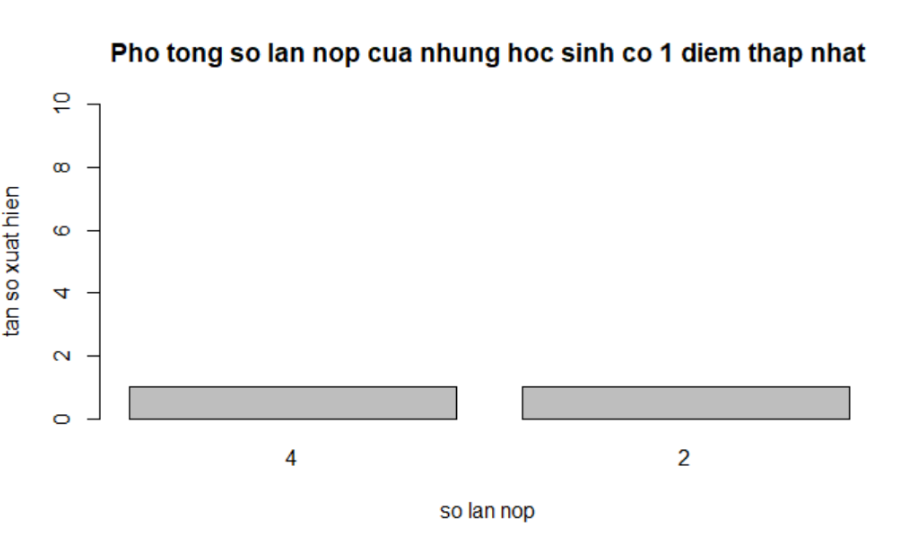
\includegraphics[scale=0.4]{Pics/q2d-file1.PNG}
    \caption{(2d) Phổ theo số lần nộp bài của sinh viên có ít nhất 1 bài nộp có điểm thấp nhất}
    \label{fig:my_label}
\end{figure}
\begin{figure}[!ht]
    \centering
    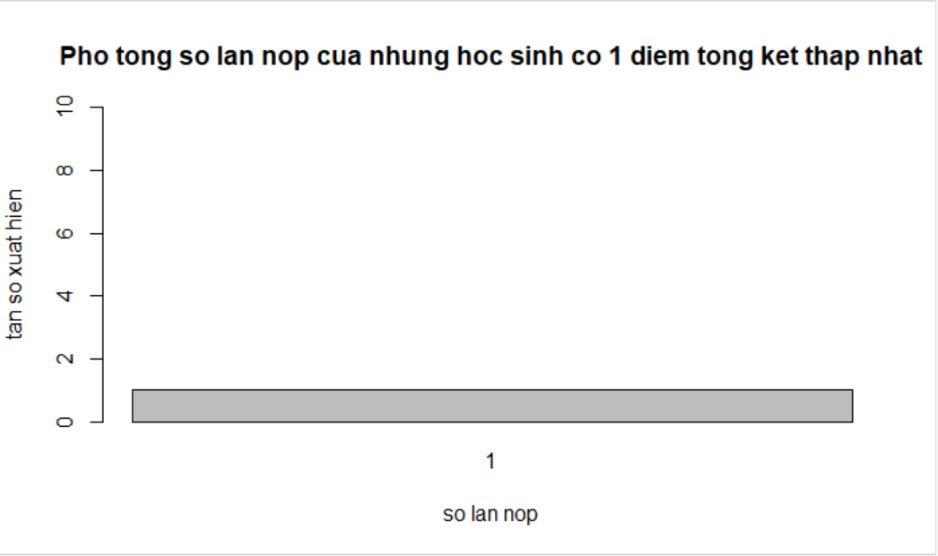
\includegraphics[scale=0.4]{Pics/q2g-file1.PNG}
    \caption{(2g) Phổ theo số lần nộp bài của các sinh viên có điểm số tổng kết thấp nhất }
    \label{fig:my_label}
\end{figure}
\newpage
\begin{figure}[!ht]
    \centering
    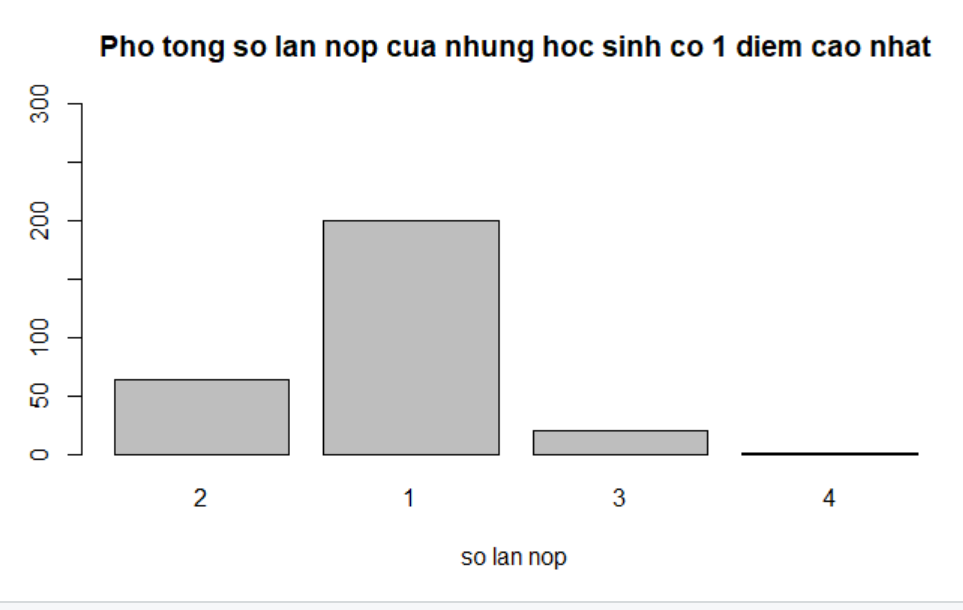
\includegraphics[scale=0.4]{Pics/q2j-file1.PNG}
    \caption{(2j)  Phổ theo số lần nộp bài của các sinh viên có tối thiểu một bài nộp có điểm số cao nhất}
    \label{fig:my_label}
\end{figure}
\begin{figure}[!ht]
    \centering
    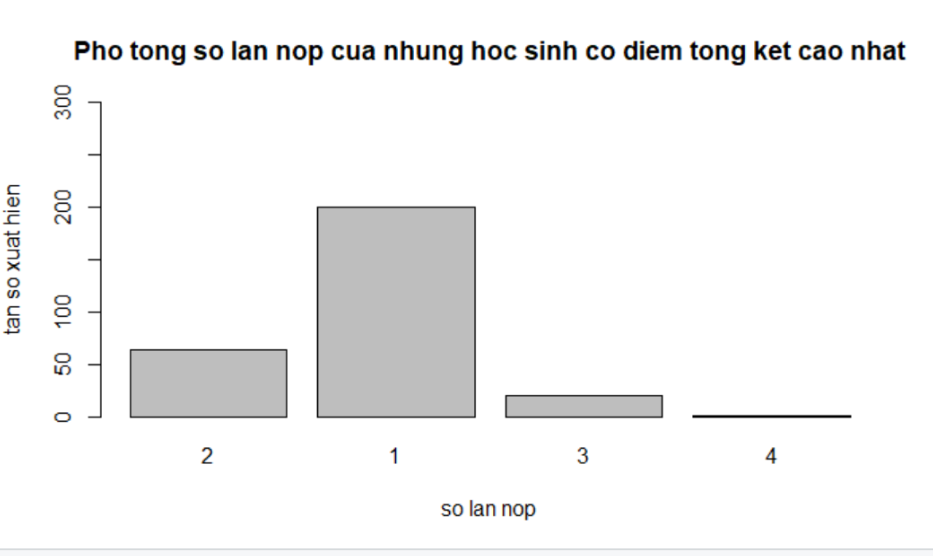
\includegraphics[scale=0.4]{Pics/q2m-file1.PNG}
    \caption{(2m) Phổ theo số lần nộp bài của các sinh viên có điểm số tổng kết cao nhấtn}
    \label{fig:my_label}
\end{figure}
\begin{figure}[!ht]
    \centering
    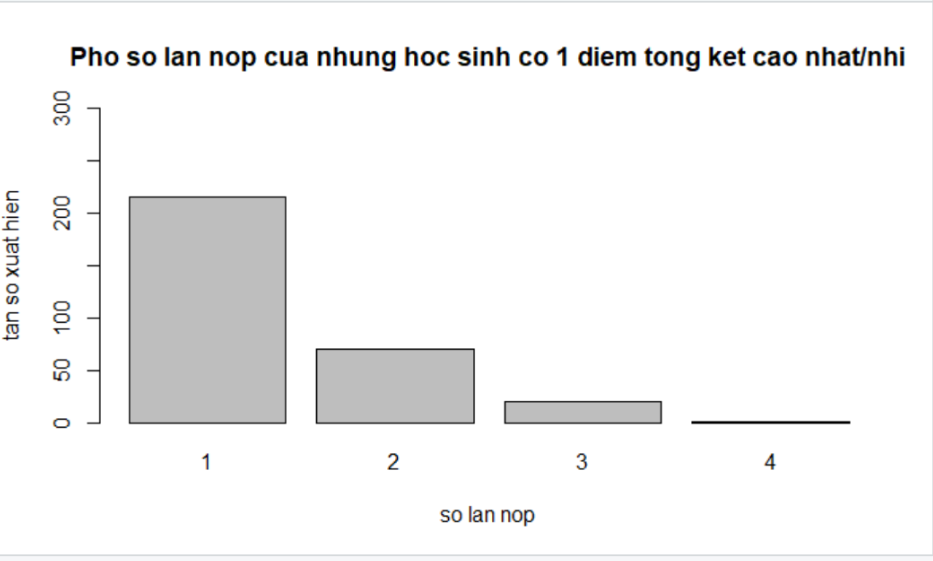
\includegraphics[scale=0.4]{Pics/q2u-file1.PNG}
    \caption{(2u) Phổ theo số lần nộp bài của các sinh viên có điểm số tổng kết ở 2 mức điểm cao nhất}
    \label{fig:my_label}
\end{figure}
\newpage 
\begin{figure}[!ht]
    \centering
    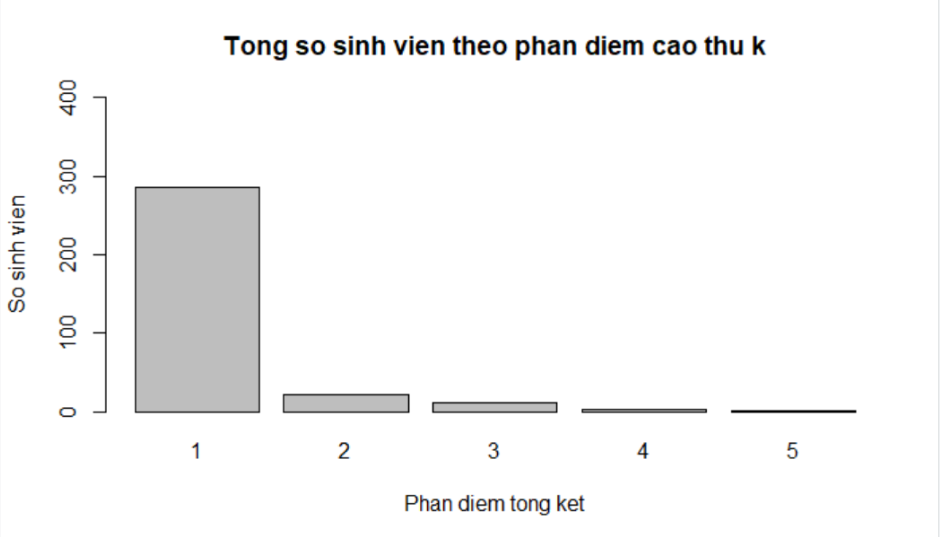
\includegraphics[scale=0.4]{Pics/q2v-file1.PNG}
    \caption{(2v) Số lượng sinh viên có điểm số tổng kết ở mức điểm cao thứ $k$ với $k$ cho trước}
    \label{fig:my_label}
\end{figure}
\begin{figure}[!ht]
    \centering
    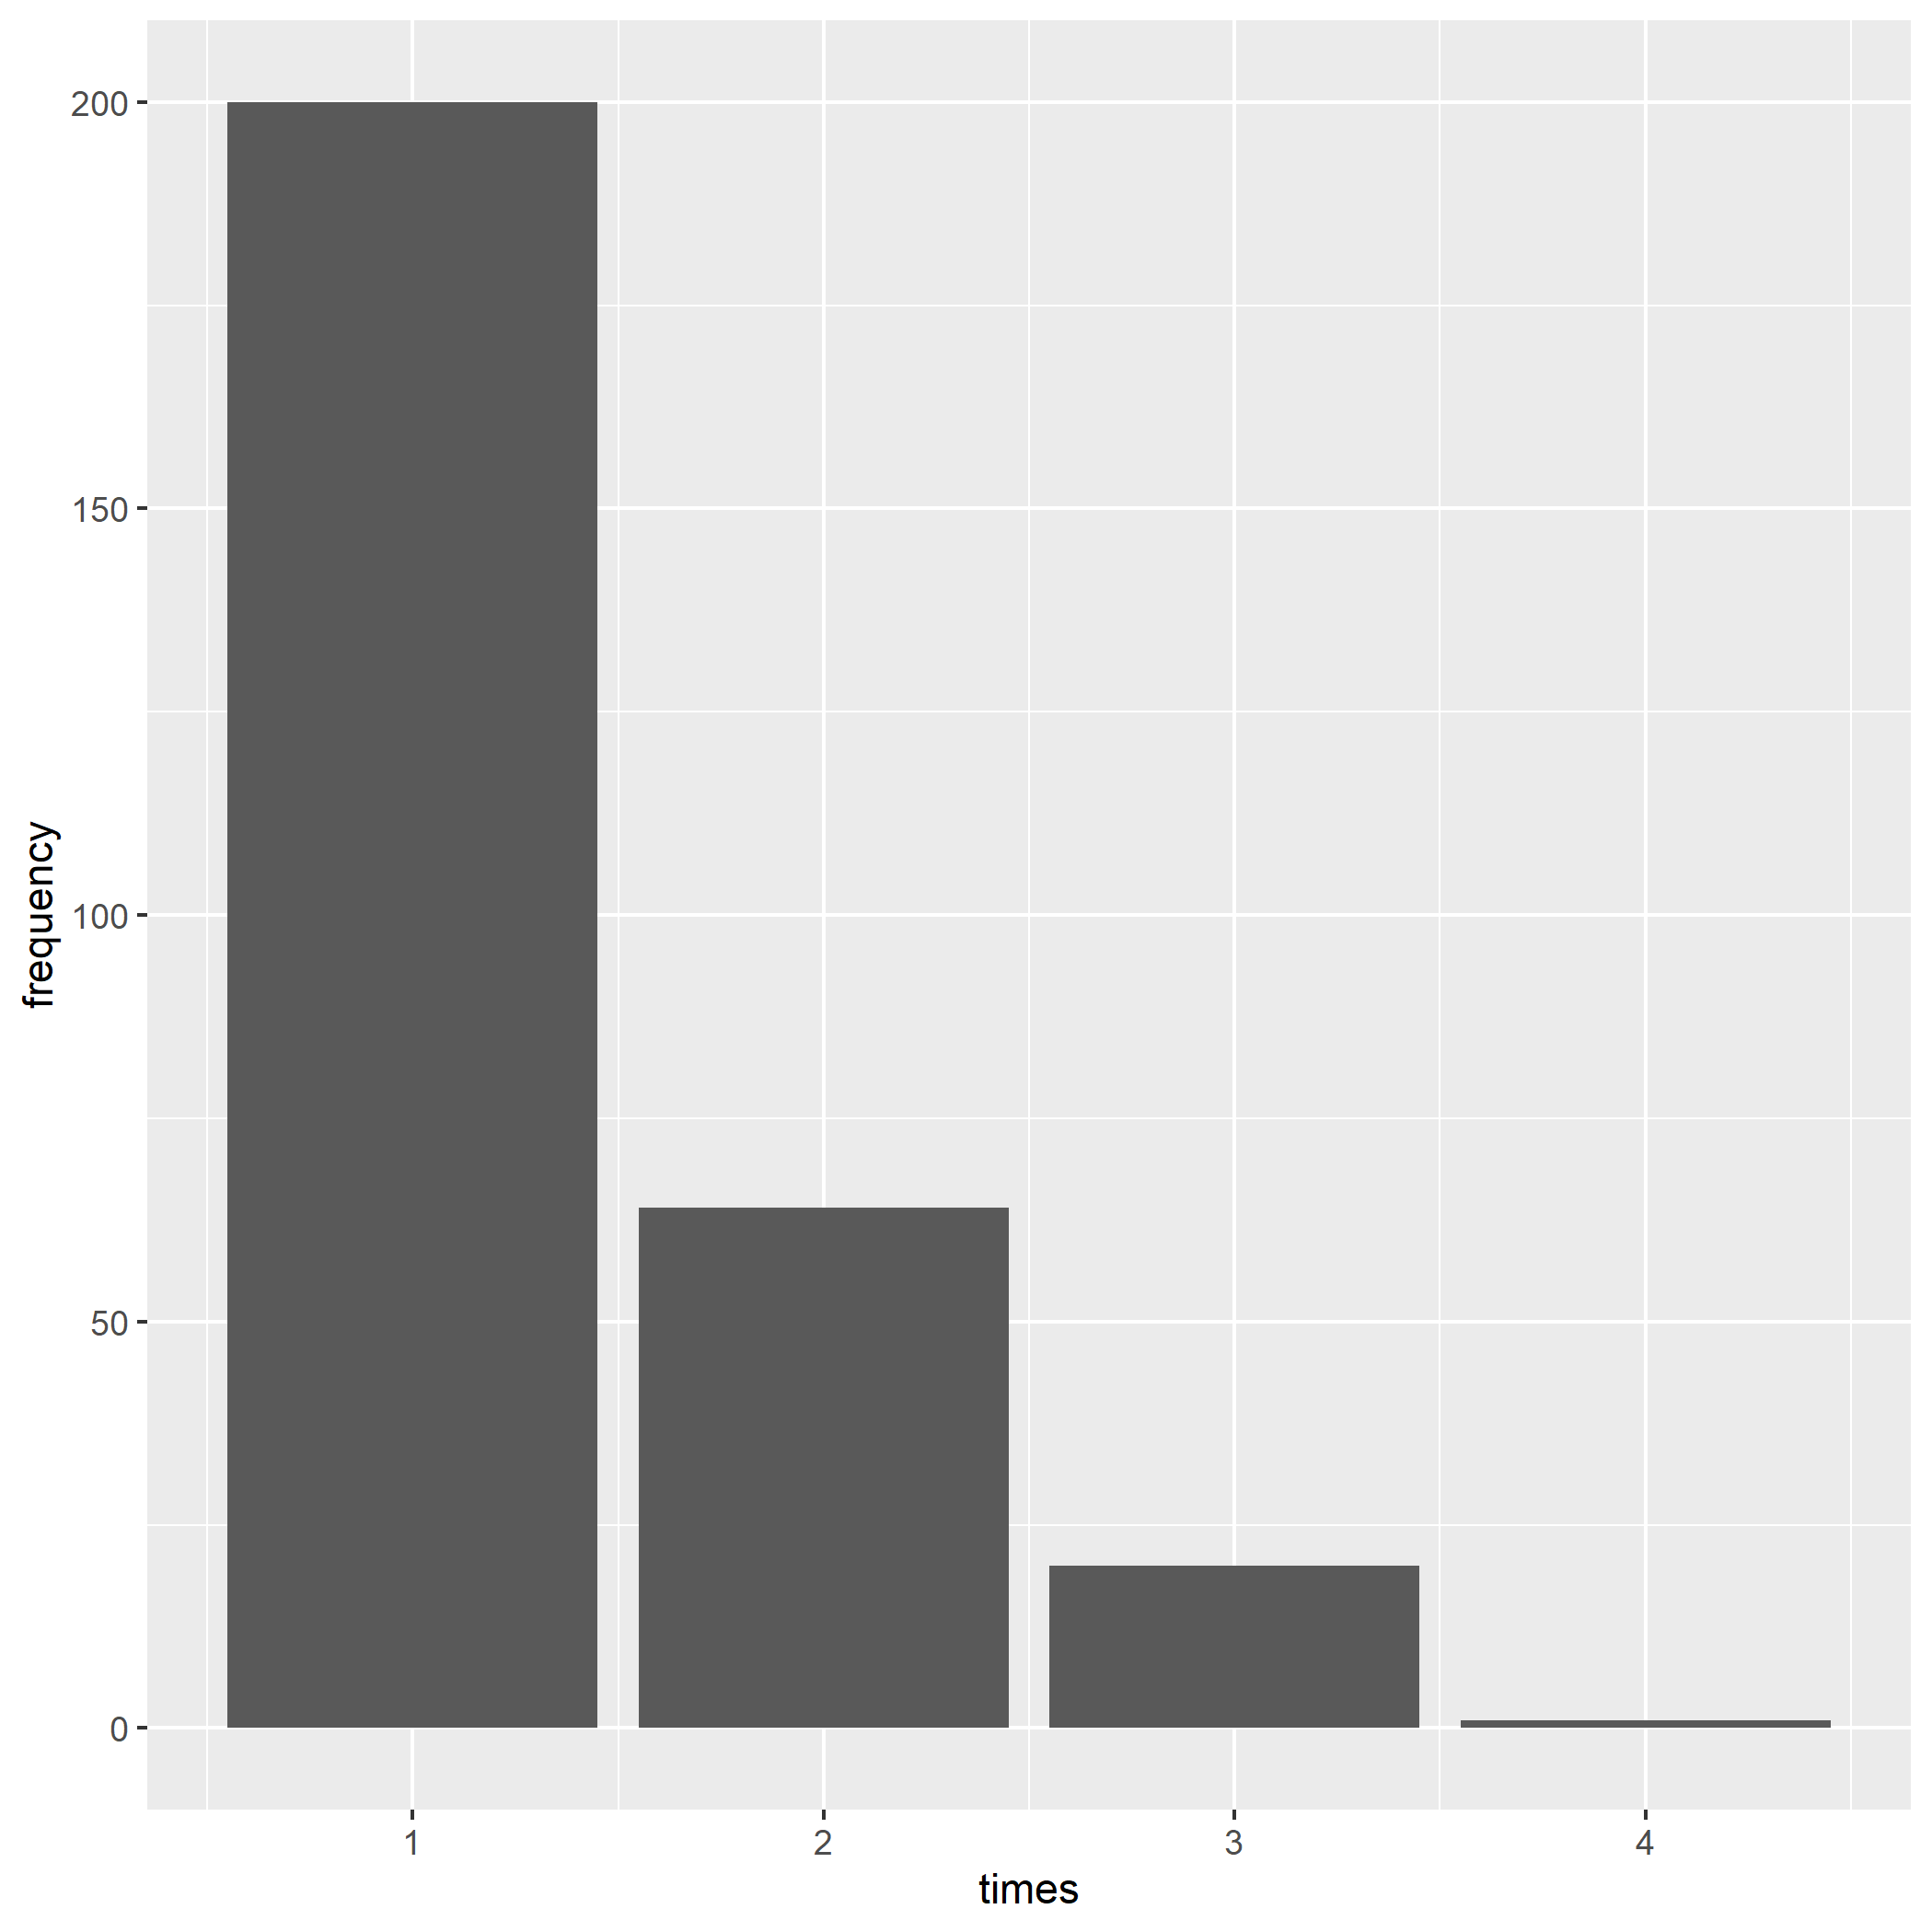
\includegraphics[scale=0.4]{Pics/q2w-1-file1.PNG}
    \caption{(2w) Phổ theo số lần nộp bài của các sinh viên có điểm số tổng kết ở mức điểm cao thứ $1$}
    \label{fig:my_label}
\end{figure}
\begin{figure}[!ht]
    \centering
    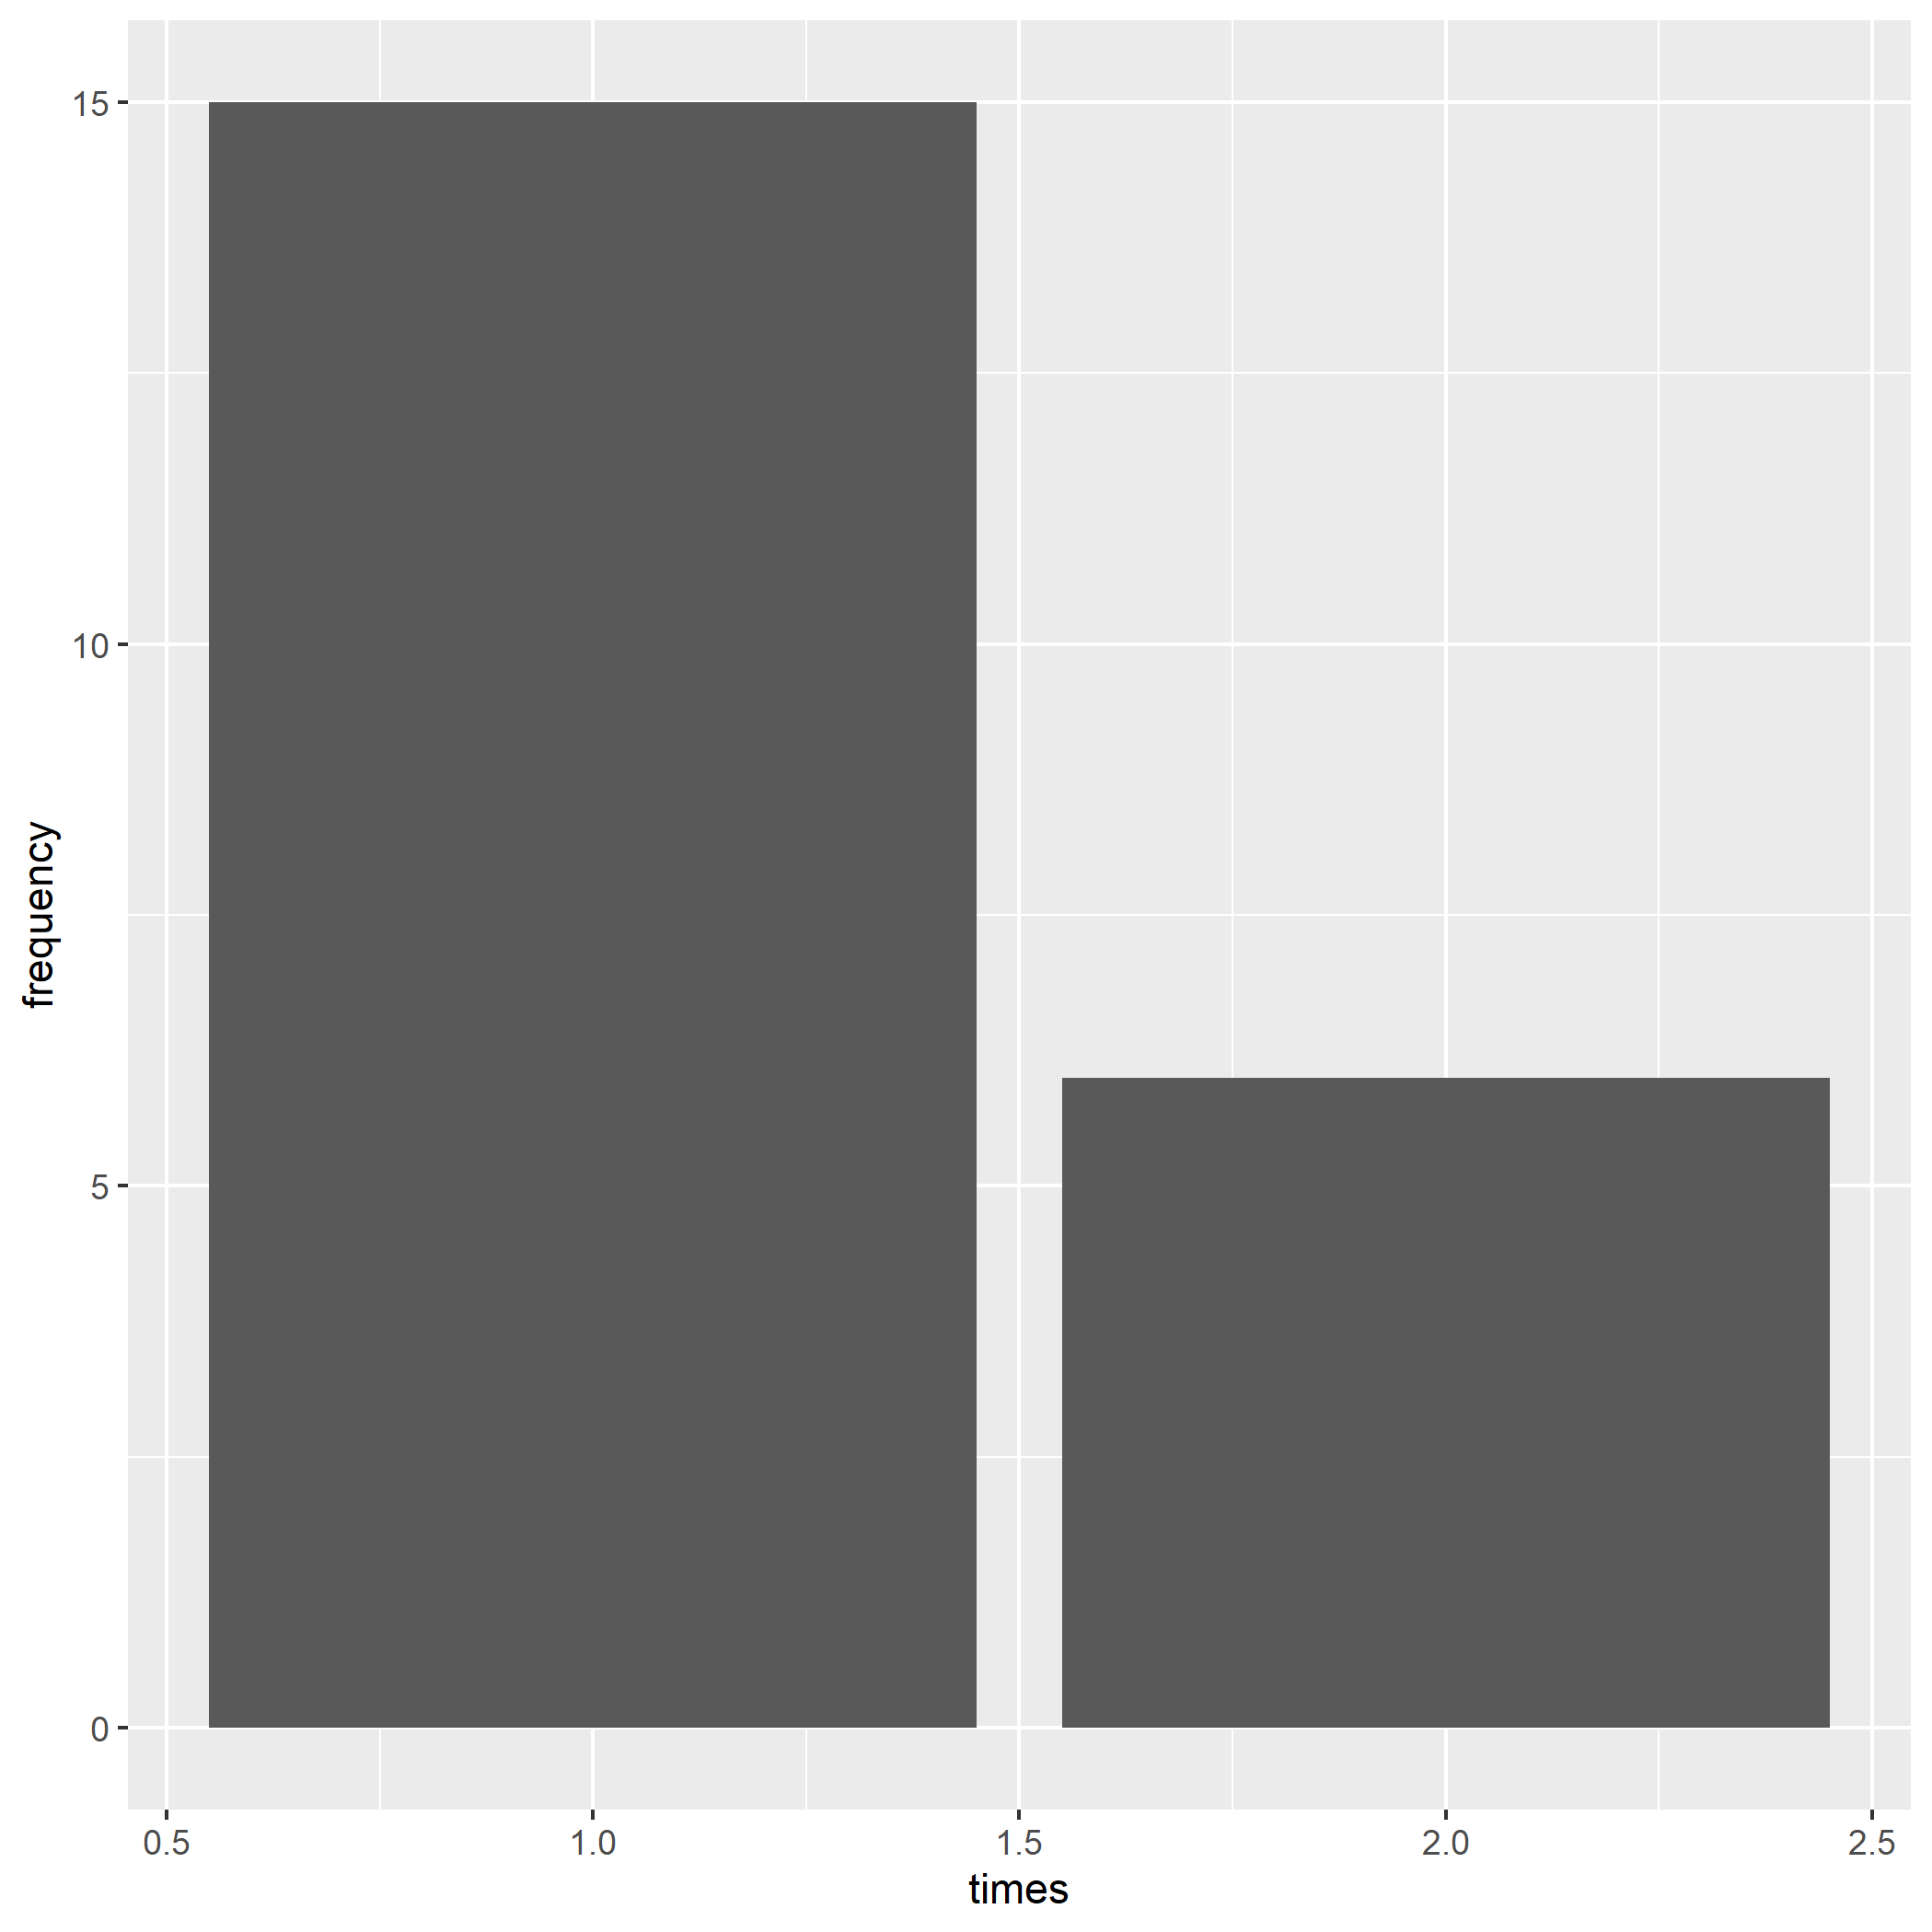
\includegraphics[scale=0.4]{Pics/q2w-2-file1.PNG}
    \caption{(2w) Phổ theo số lần nộp bài của các sinh viên có điểm số tổng kết ở mức điểm cao thứ $2$}
    \label{fig:my_label}
\end{figure}
\begin{figure}[!ht]
    \centering
    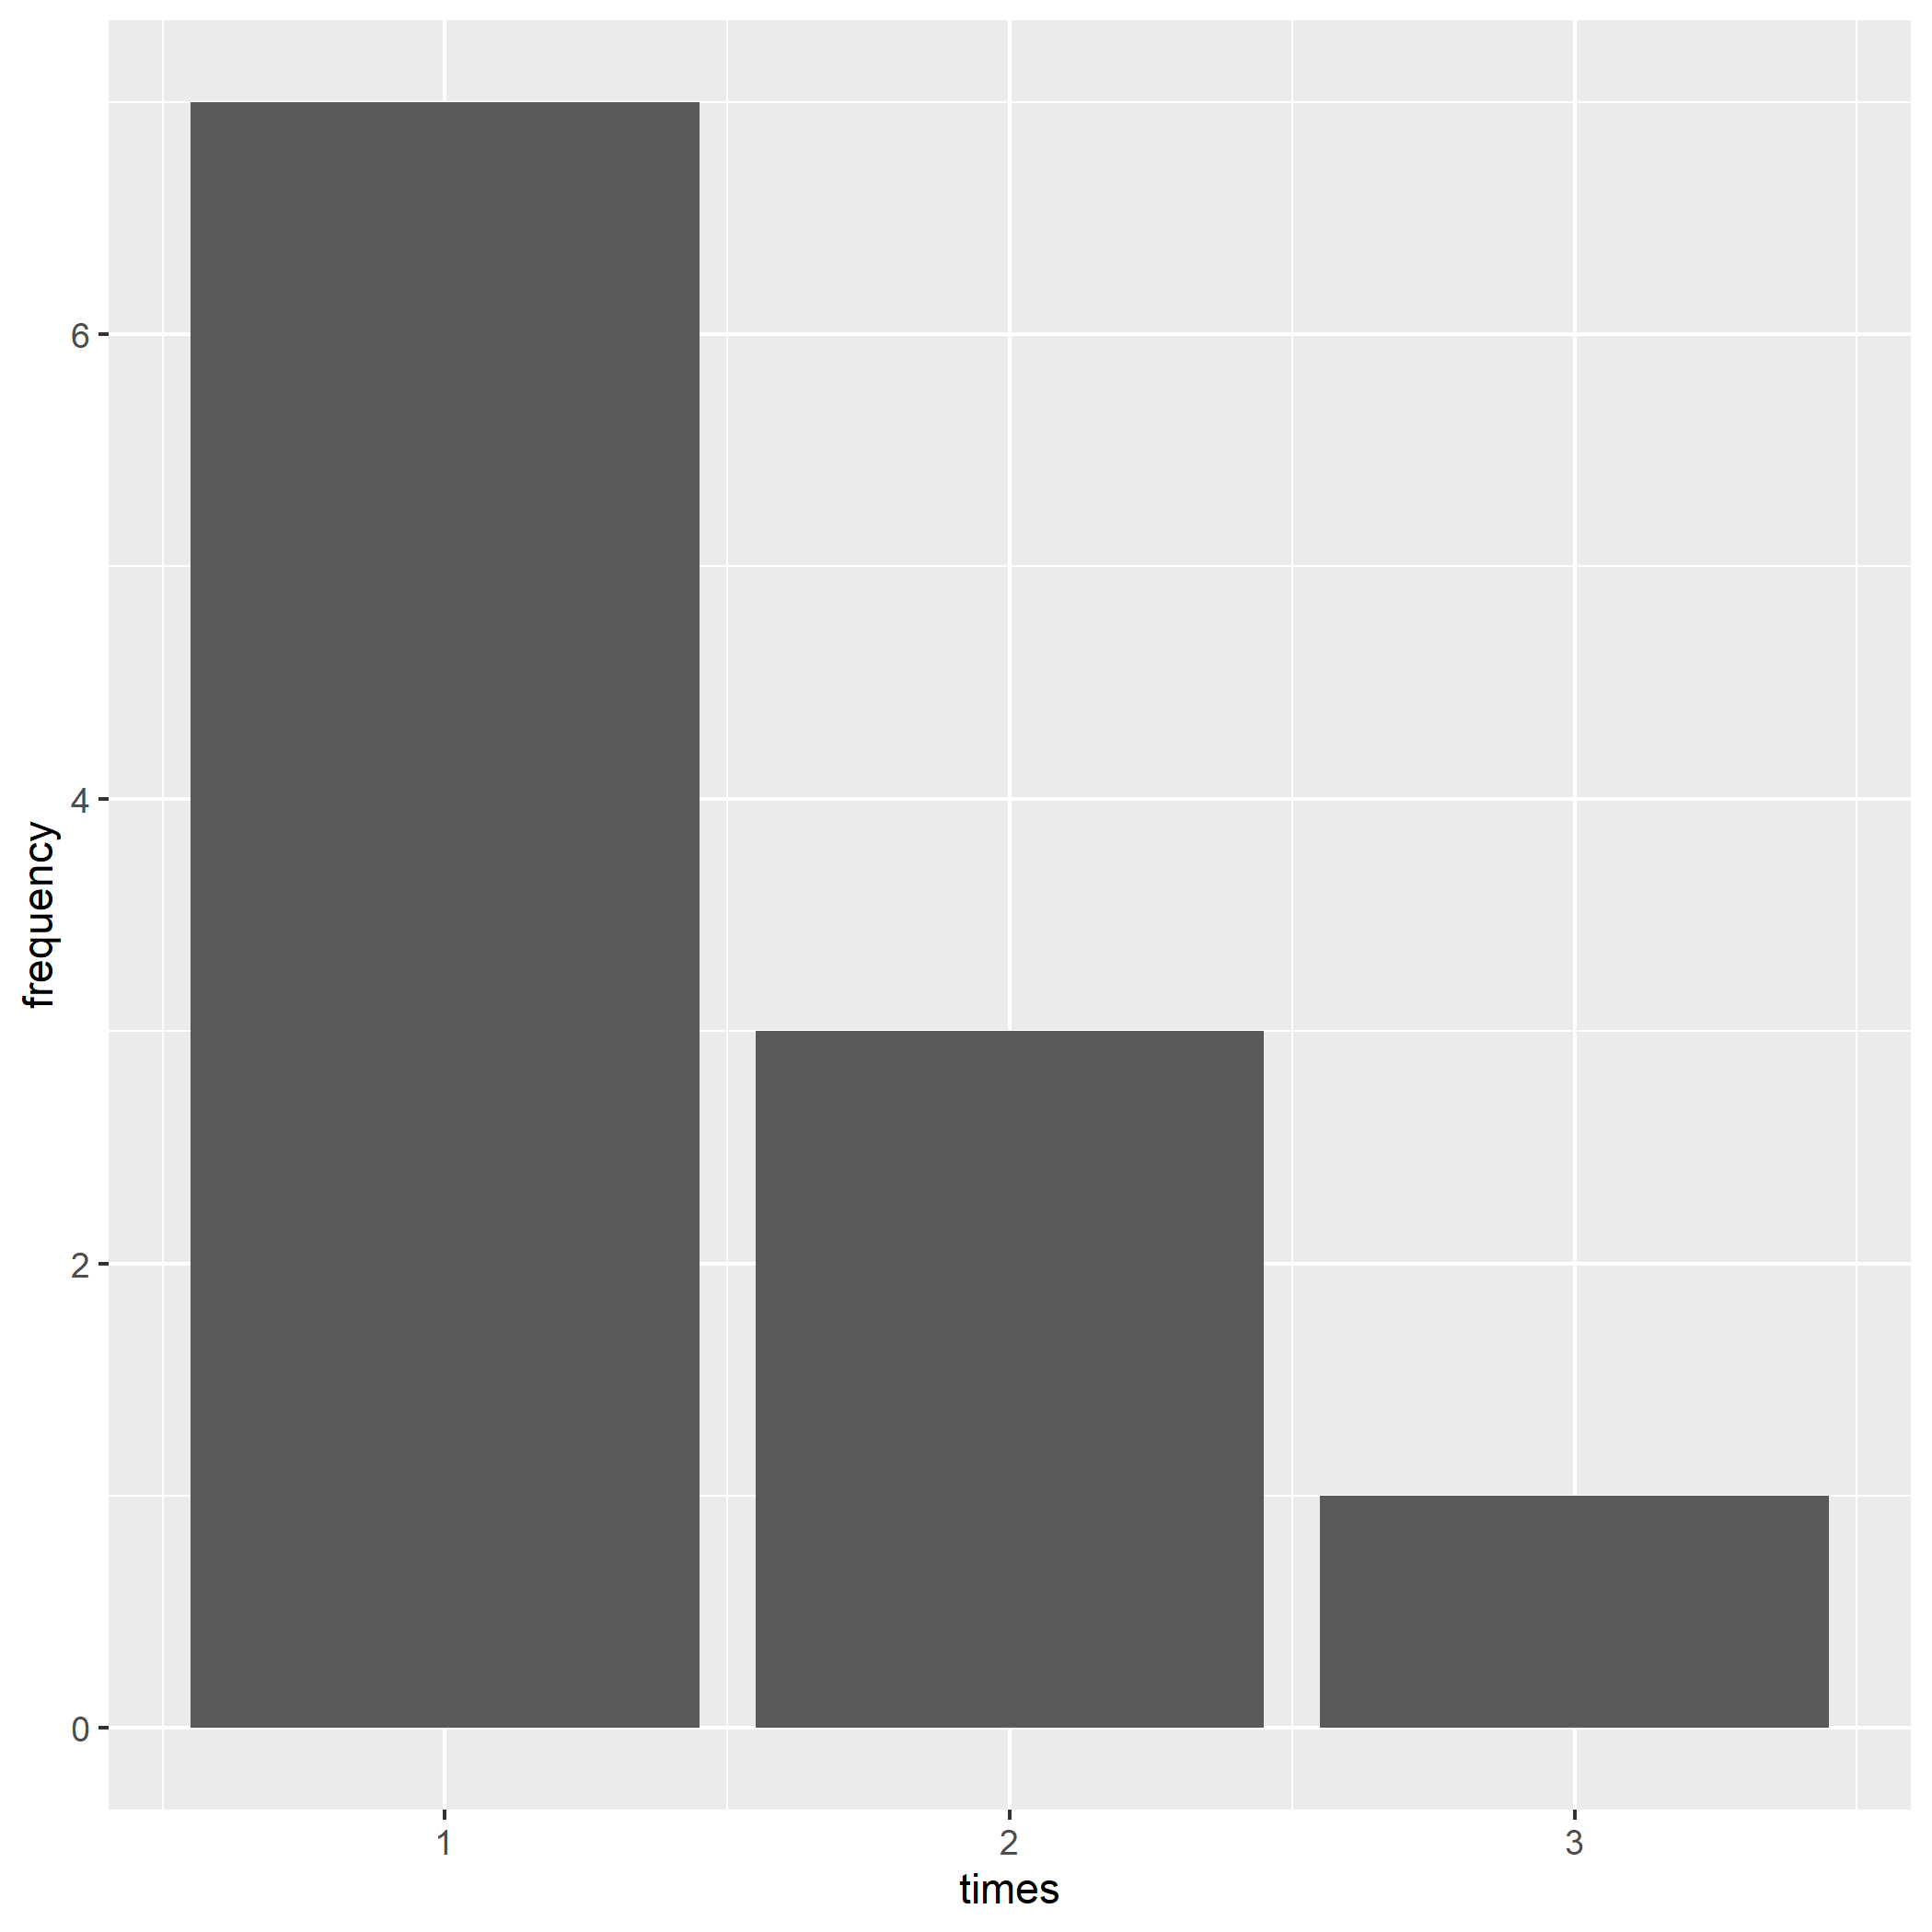
\includegraphics[scale=0.4]{Pics/q2w-3-file1.PNG}
    \caption{(2w) Phổ theo số lần nộp bài của các sinh viên có điểm số tổng kết ở mức điểm cao thứ $3$}
    \label{fig:my_label}
\end{figure}
\begin{figure}[!ht]
    \centering
    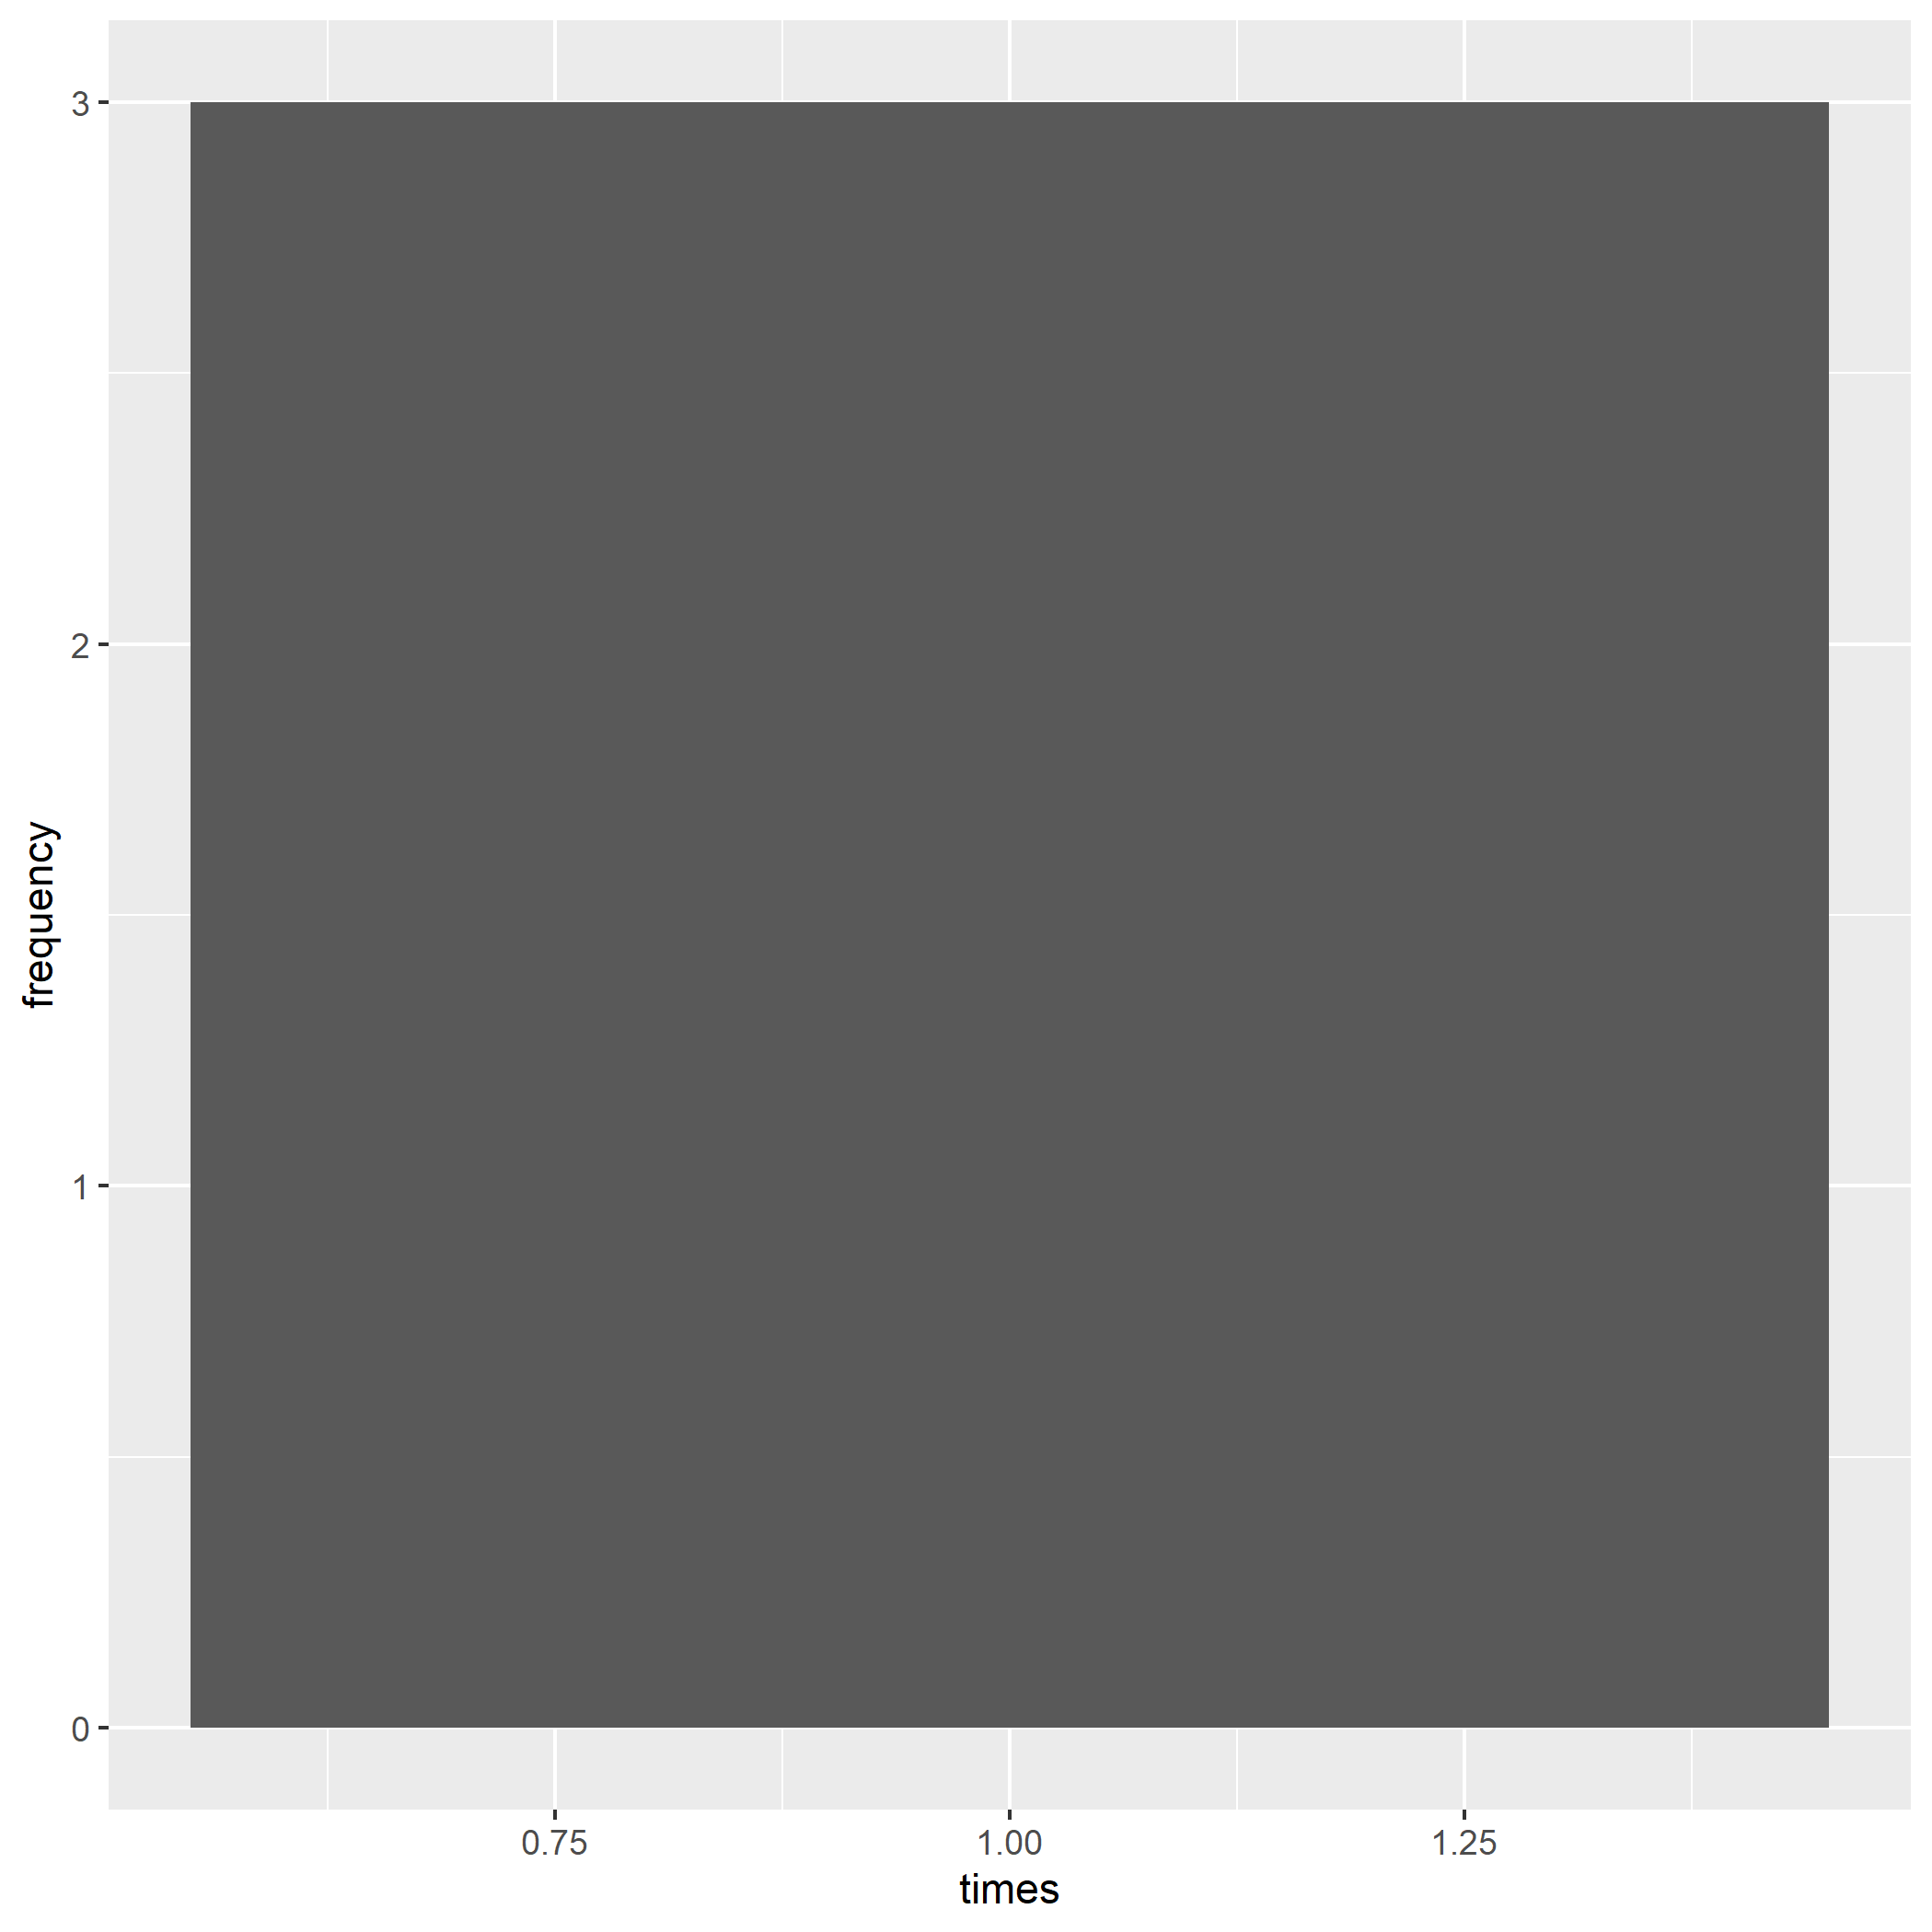
\includegraphics[scale=0.4]{Pics/q2w-4-file1.png}
    \caption{(2w) Phổ theo số lần nộp bài của các sinh viên có điểm số tổng kết ở mức điểm cao thứ $4$}
    \label{fig:my_label}
\end{figure}
\begin{figure}[!ht]
    \centering
    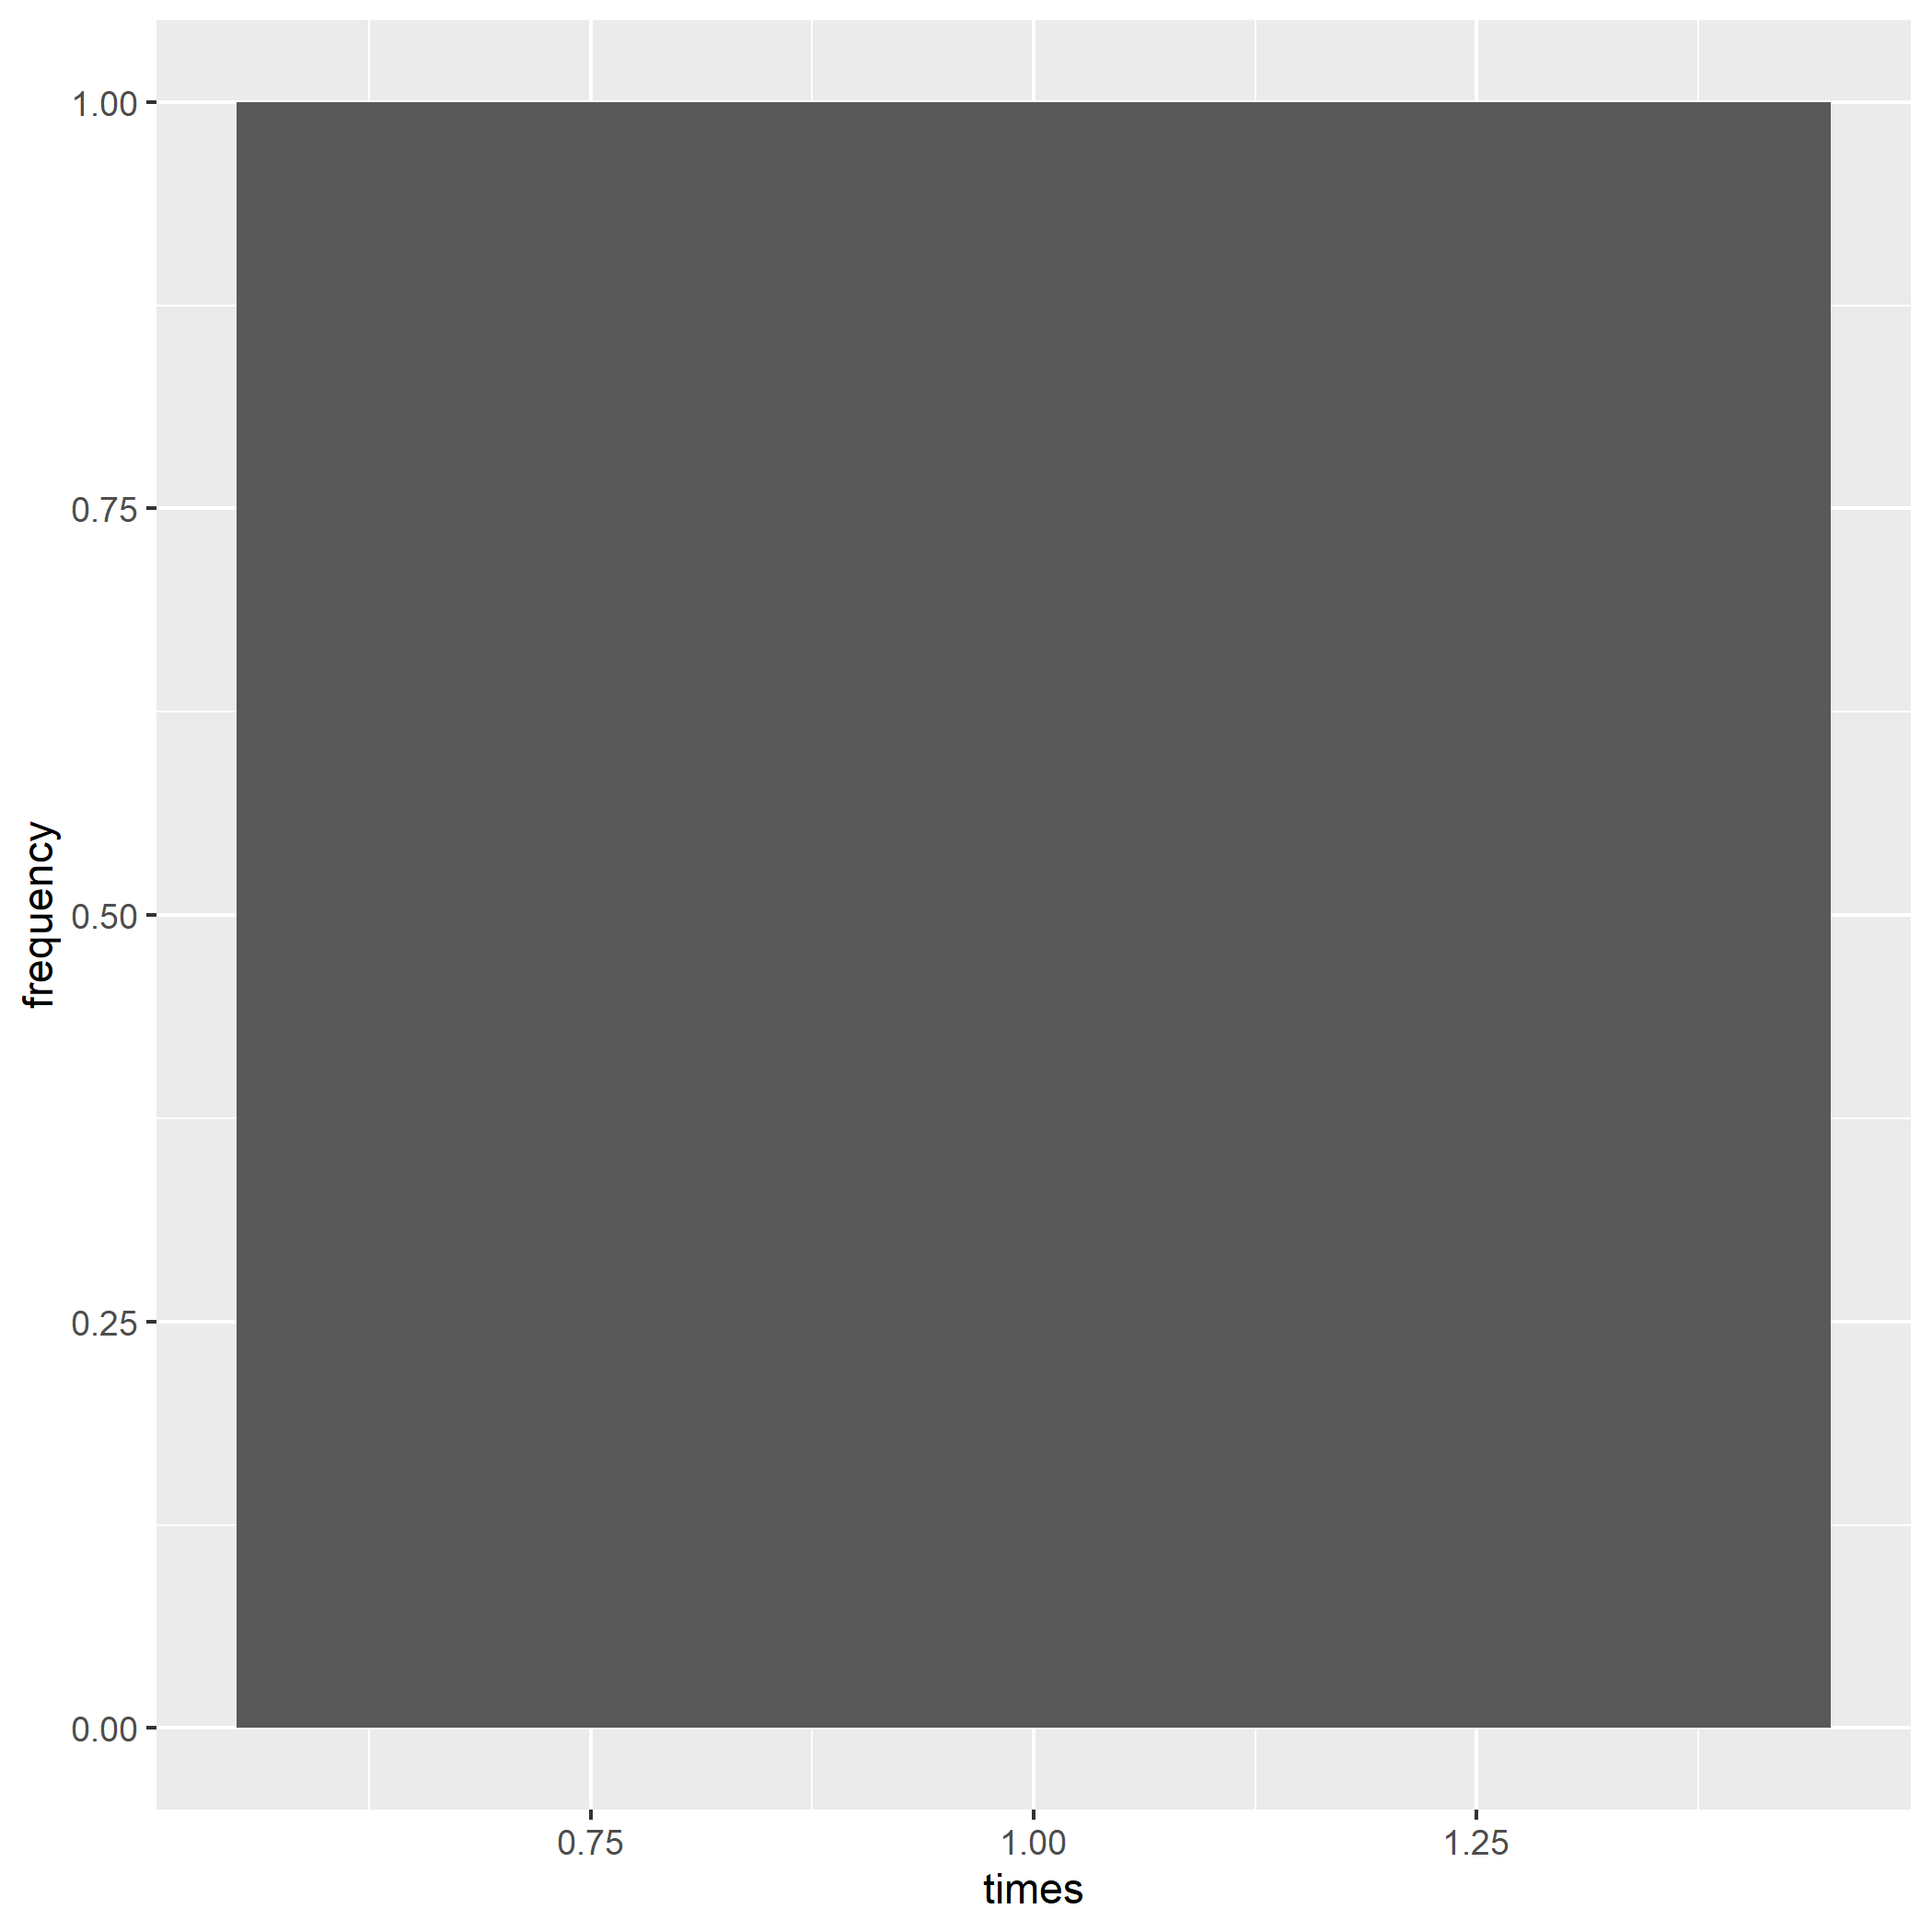
\includegraphics[scale=0.4]{Pics/q2w-5-file1.png}
    \caption{(2w)Phổ theo số lần nộp bài của các sinh viên có điểm số tổng kết ở mức điểm cao thứ $5$}
    \label{fig:my_label}
\end{figure}
\newpage



\subsubsection{Câu 3}
\newpage



\subsubsection{Câu 4}
\begin{figure}[!ht]
    \centering
    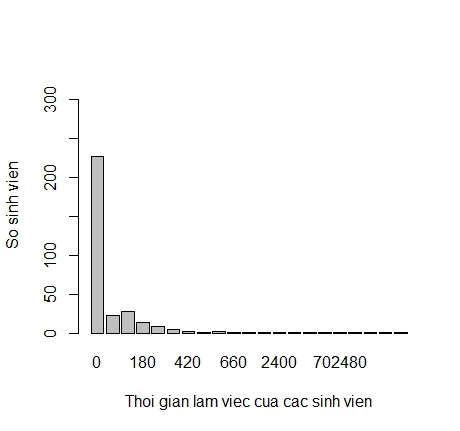
\includegraphics[scale=0.4]{Pics/q4b-file1.jpeg}
    \caption{(4b) Phổ thời gian làm việc (được tính từ lần nộp bài đầu tiên đến lần nộp cuối) của các
sinh viên.}
    \label{fig:my_label}
\end{figure}
\newpage
\begin{figure}[!ht]
    \centering
    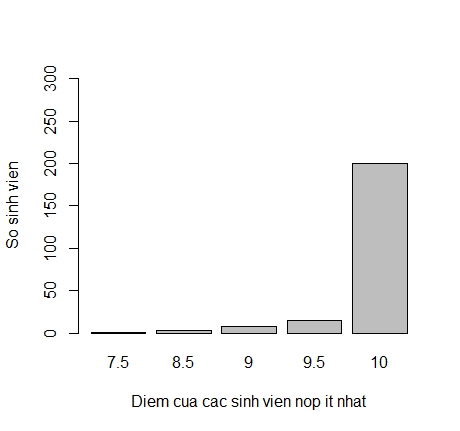
\includegraphics[scale=0.4]{Pics/q4e-file1.jpeg}
    \caption{(4e) Phổ điểm của các sinh viên có tần suất nộp bài ít nhất}
    \label{fig:my_label}
\end{figure}
\begin{figure}[!ht]
    \centering
    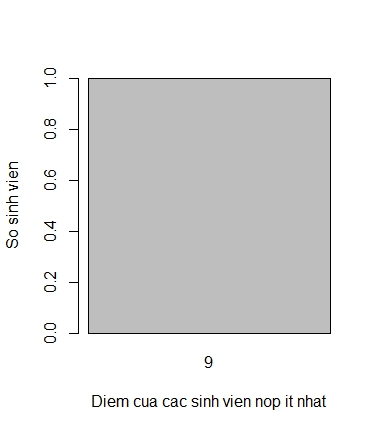
\includegraphics[scale=0.4]{Pics/q4h-file1.jpeg}
    \caption{(4h) Phổ điểm của các sinh viên có tần suất nộp bài nhiều nhất}
    \label{fig:my_label}
\end{figure}
\begin{figure}[!ht]
    \centering
    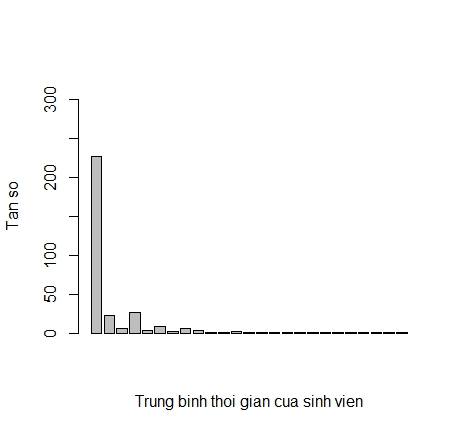
\includegraphics[scale=0.4]{Pics/q4m-file1.jpeg}
    \caption{(4m) Biểu đồ tần số của mẫu}
    \label{fig:my_label}
\end{figure}
\begin{figure}[!ht]
    \centering
    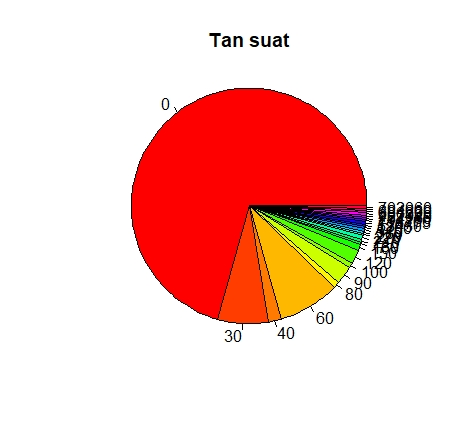
\includegraphics[scale=0.4]{Pics/q4n-file1.jpeg}
    \caption{(4n) Biểu đồ tần suất của mẫu}
    \label{fig:my_label}
\end{figure}
\newpage
\begin{figure}[!ht]
    \centering
    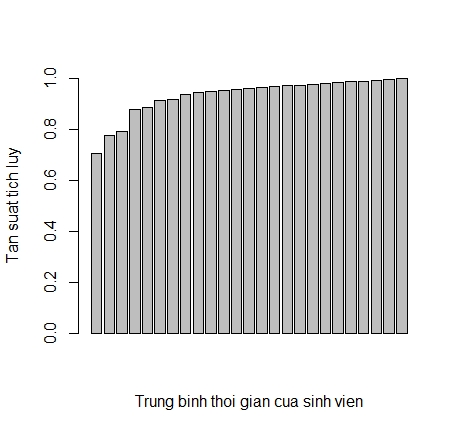
\includegraphics[scale=0.4]{Pics/q4o-file1.jpeg}
    \caption{(4o) Biểu đồ tần suất tích lũy của mẫu }
    \label{fig:my_label}
\end{figure}
\newpage
\subsubsection{Câu 5}
\begin{figure}[!ht]
    \centering
    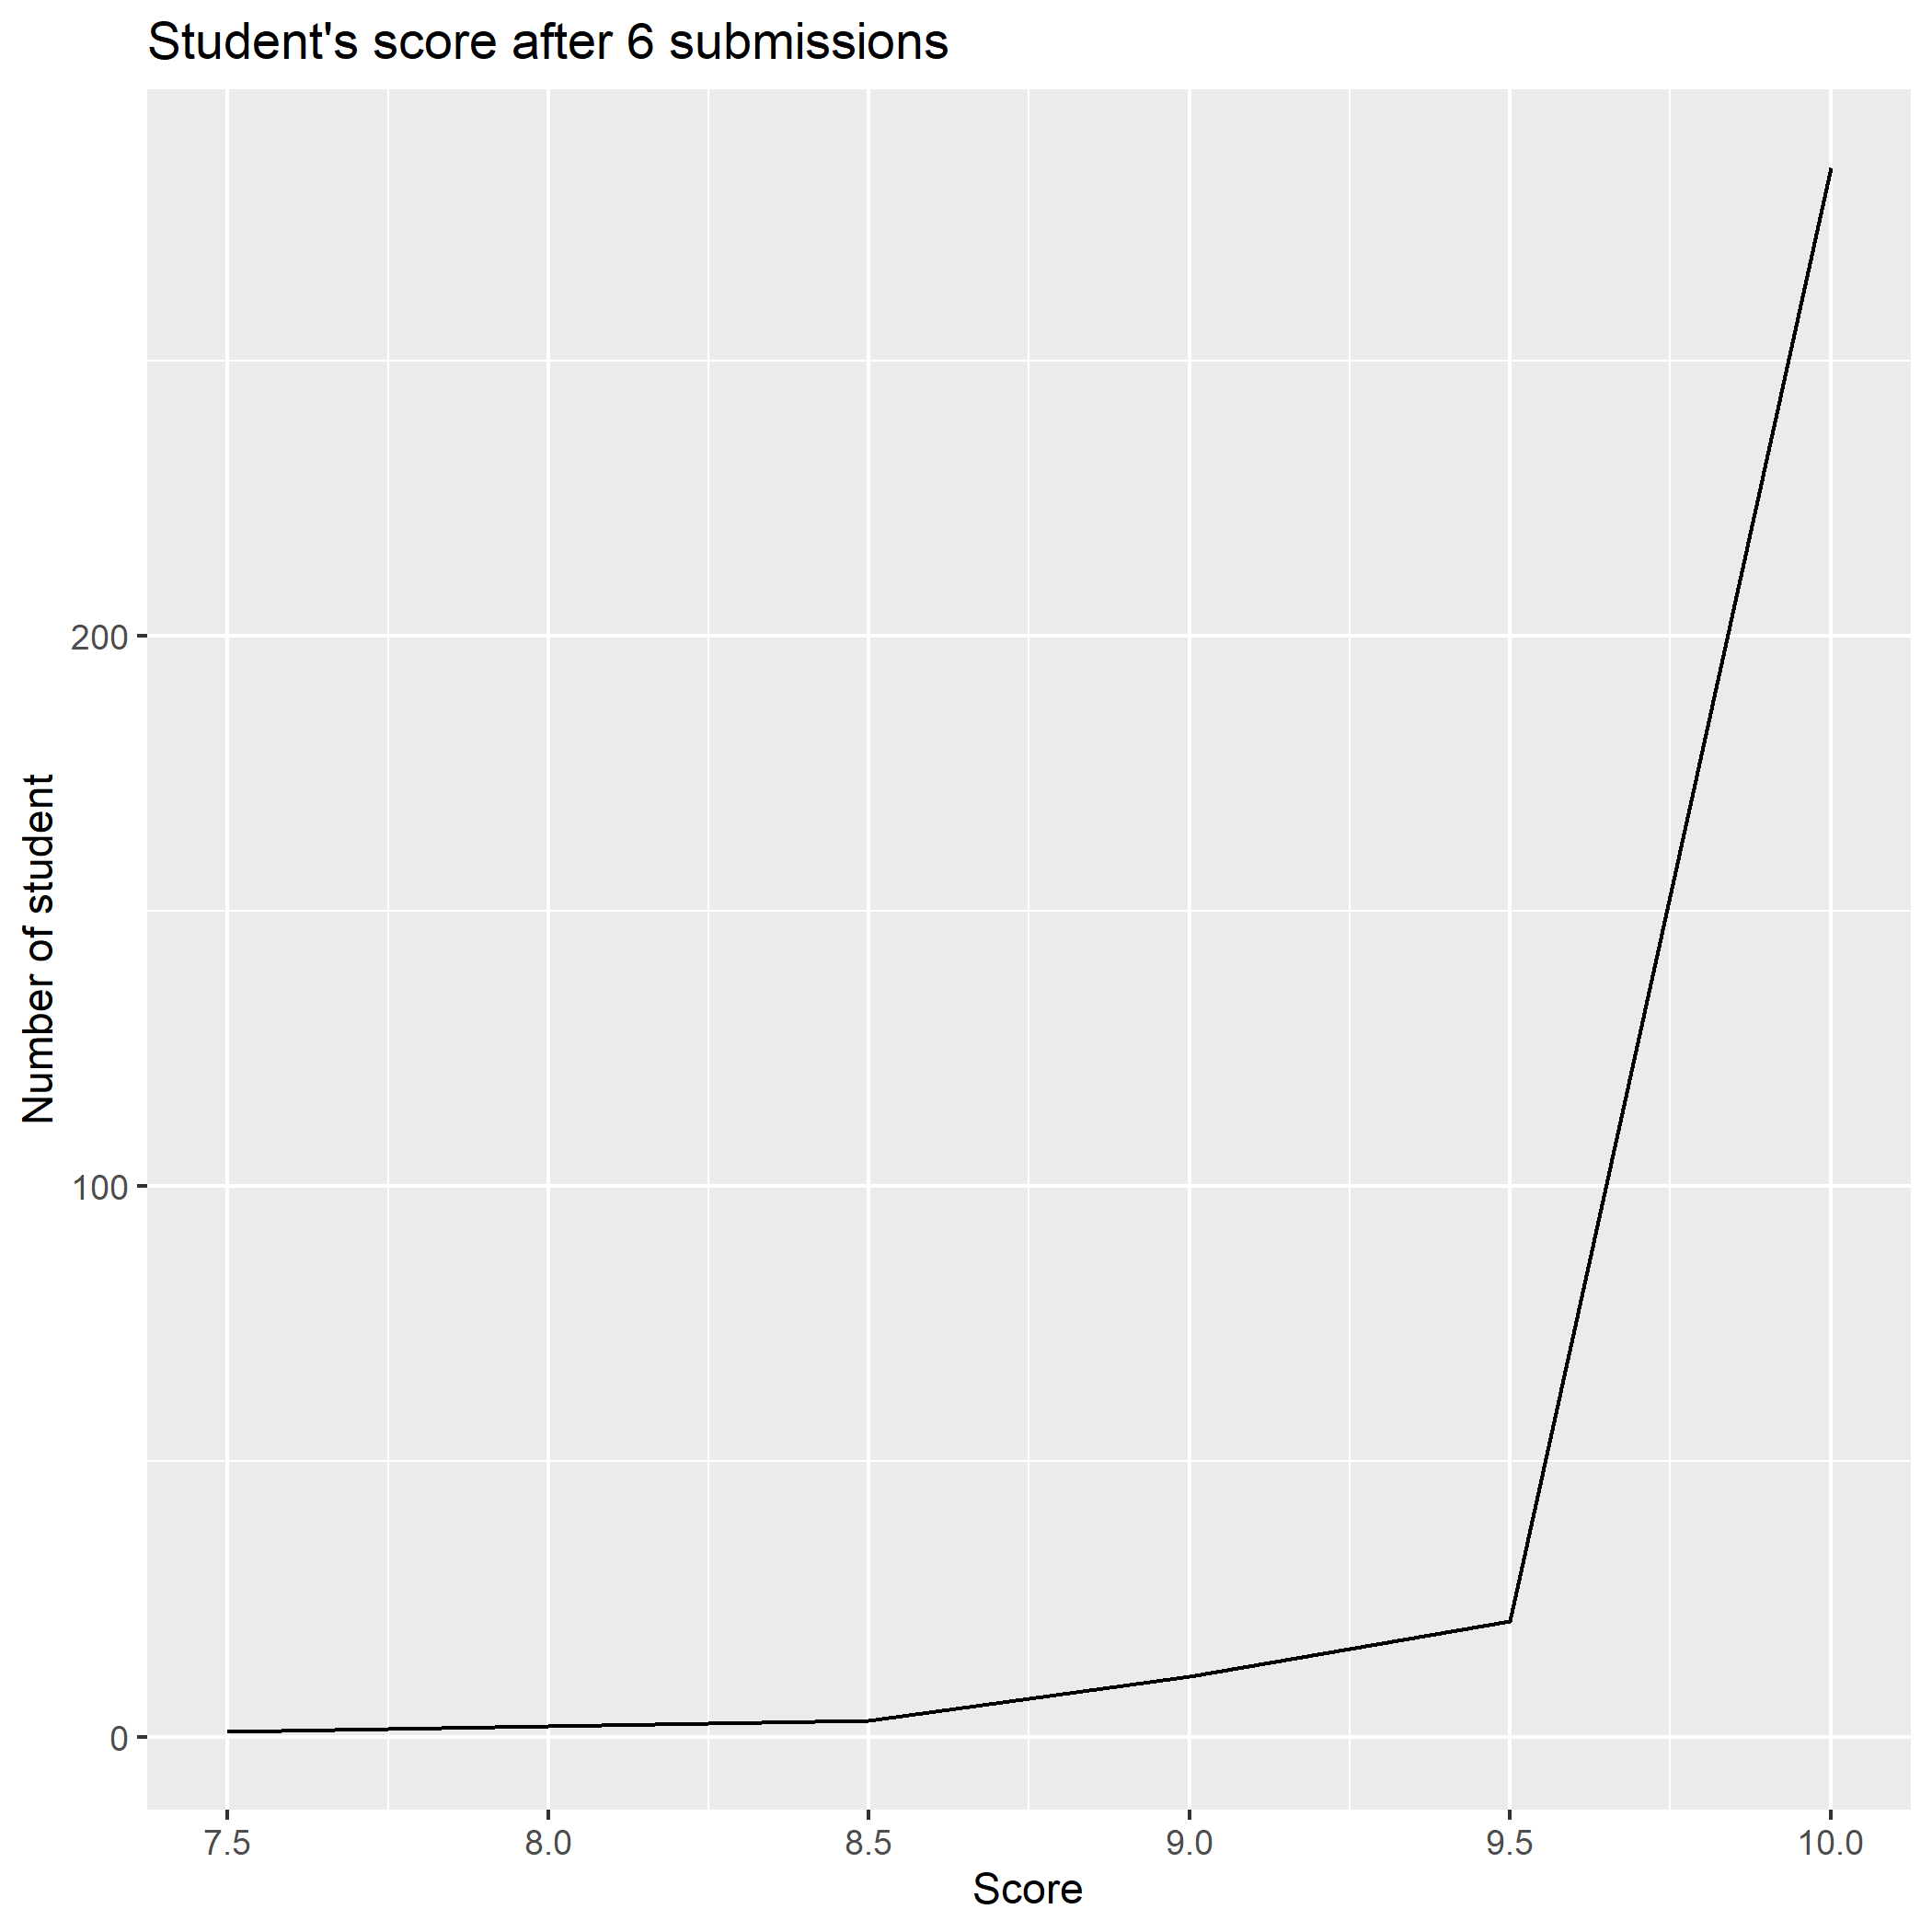
\includegraphics[scale=0.4]{Pics/q5a_file1.png}
    \caption{(5a) Điểm sinh viên sau 6 lần nộp}
    \label{fig:my_label}
\end{figure}
\begin{figure}[!ht]
    \centering
    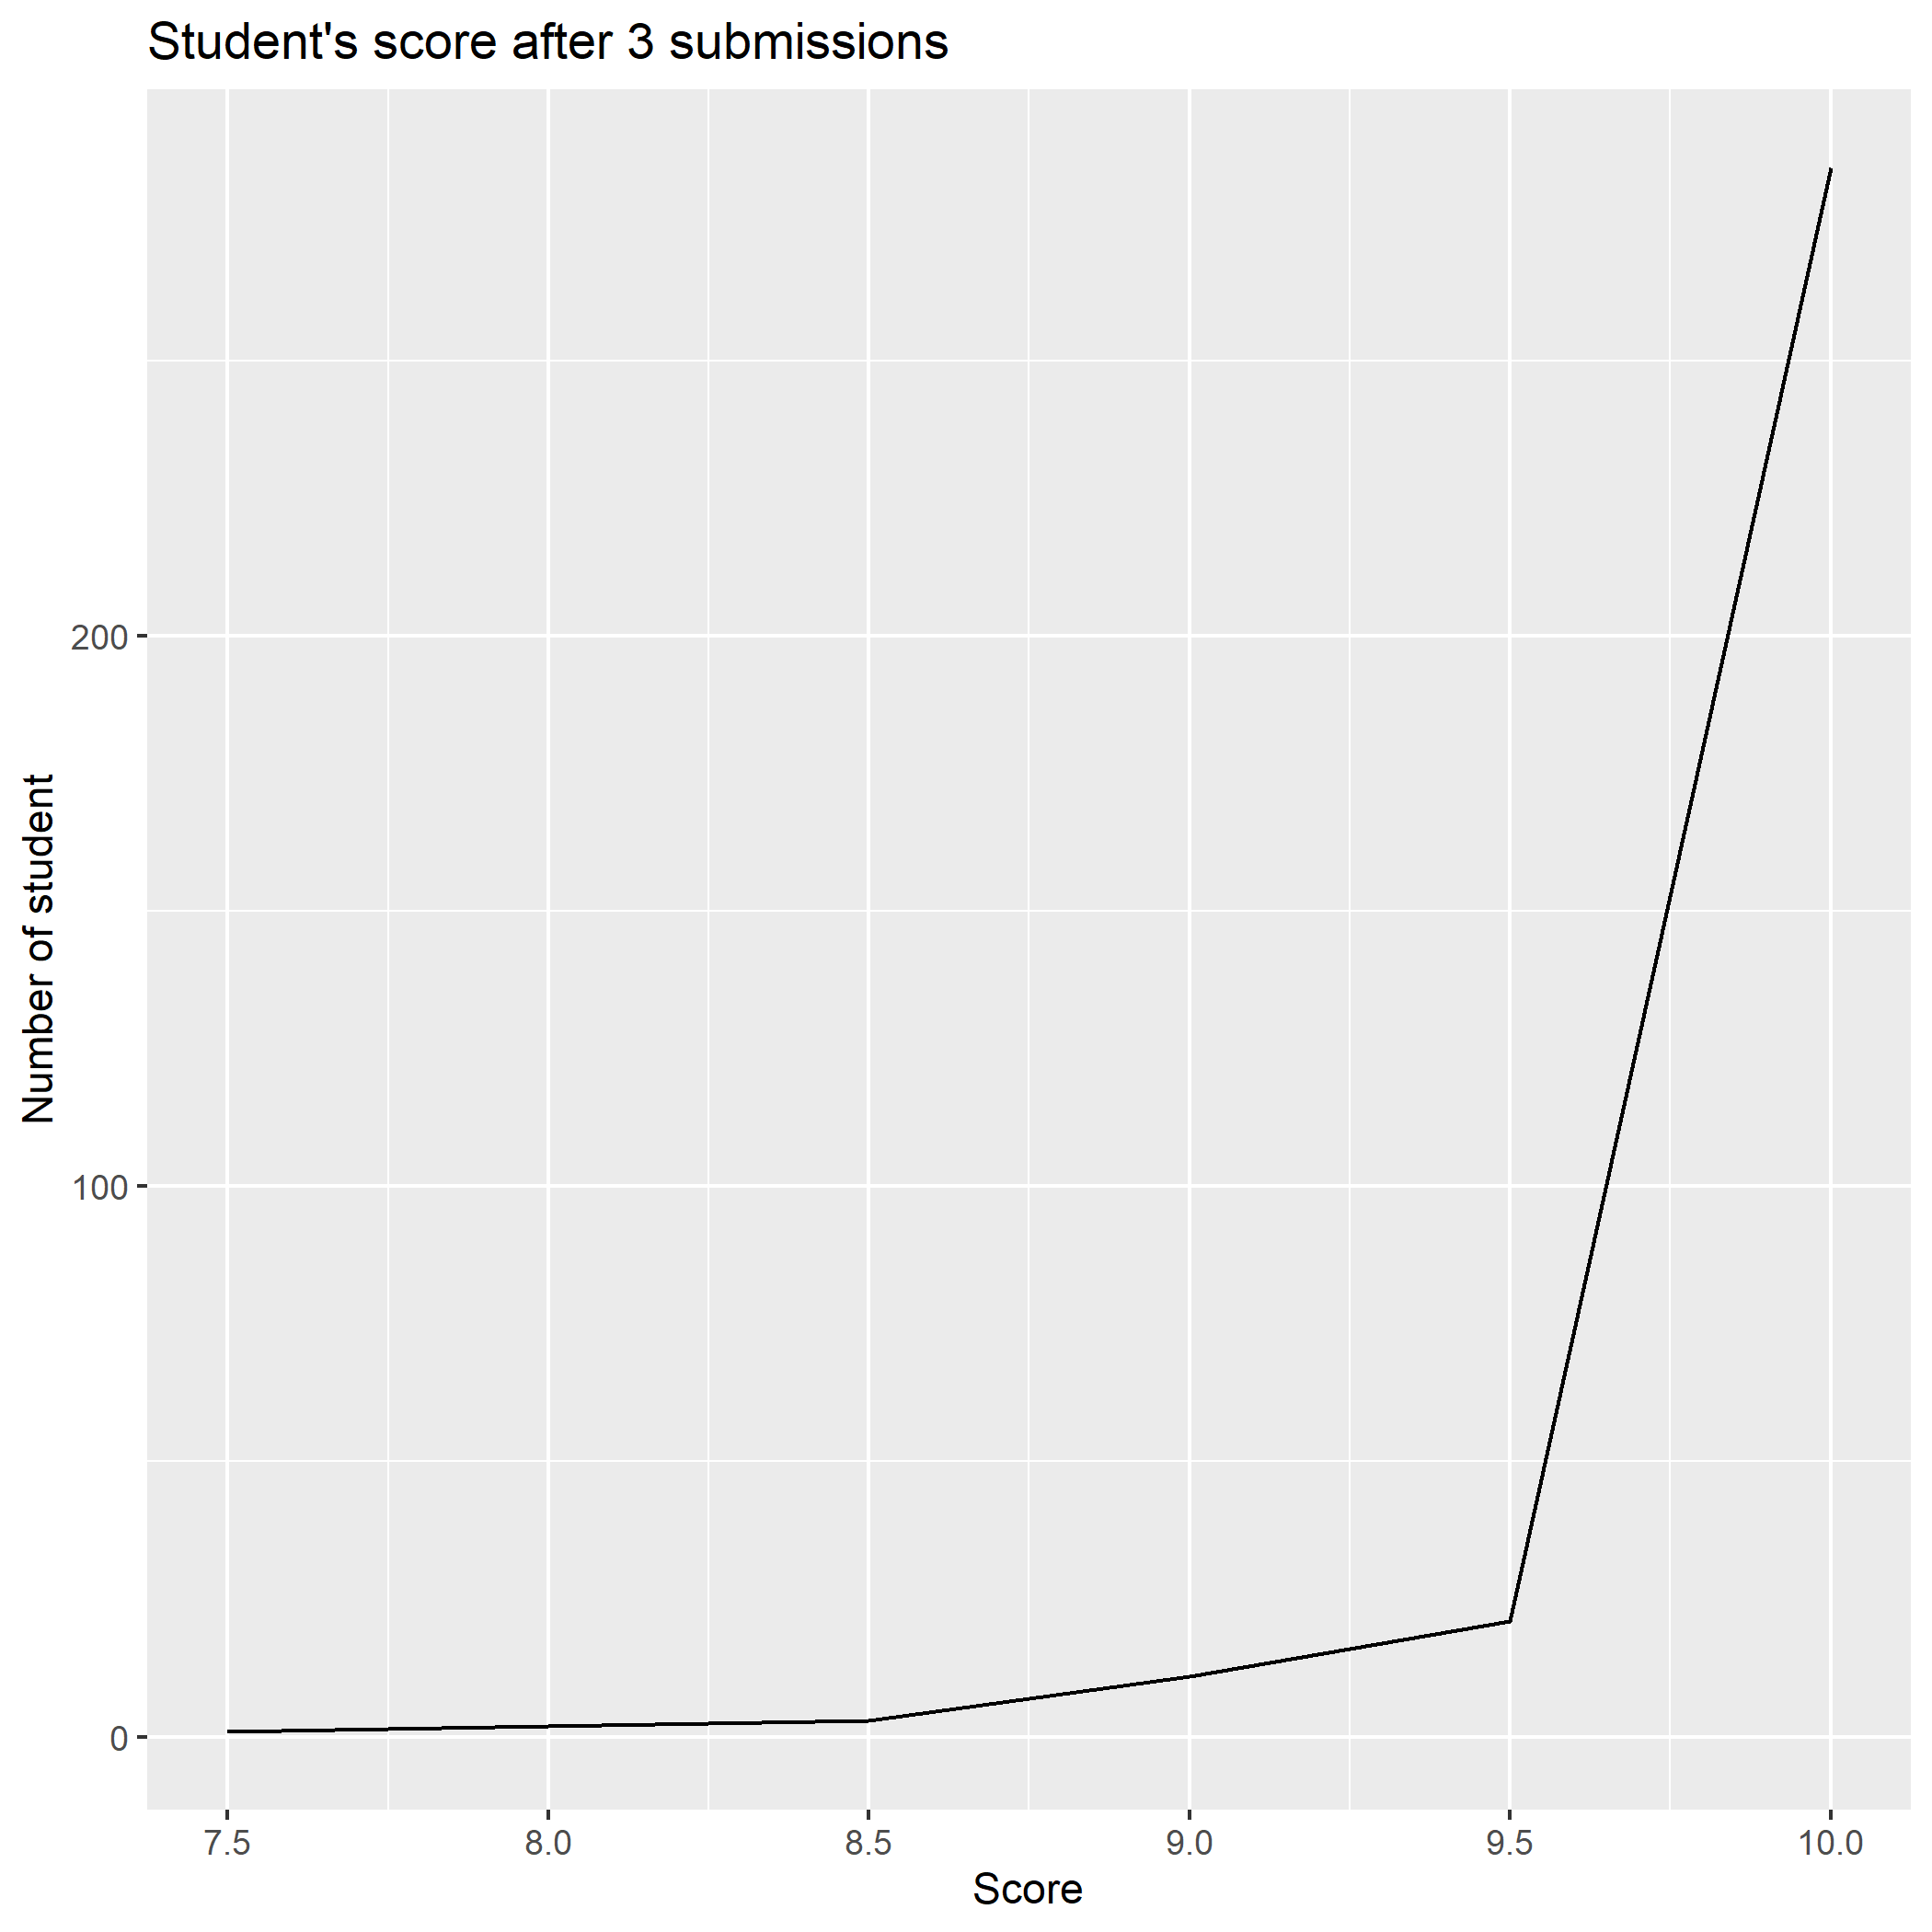
\includegraphics[scale=0.4]{Pics/q5b_file1.png}
    \caption{(5b) Điểm sinh viên sau 3 lần nộp}
    \label{fig:my_label}
\end{figure}
\begin{figure}[!ht]
    \centering
    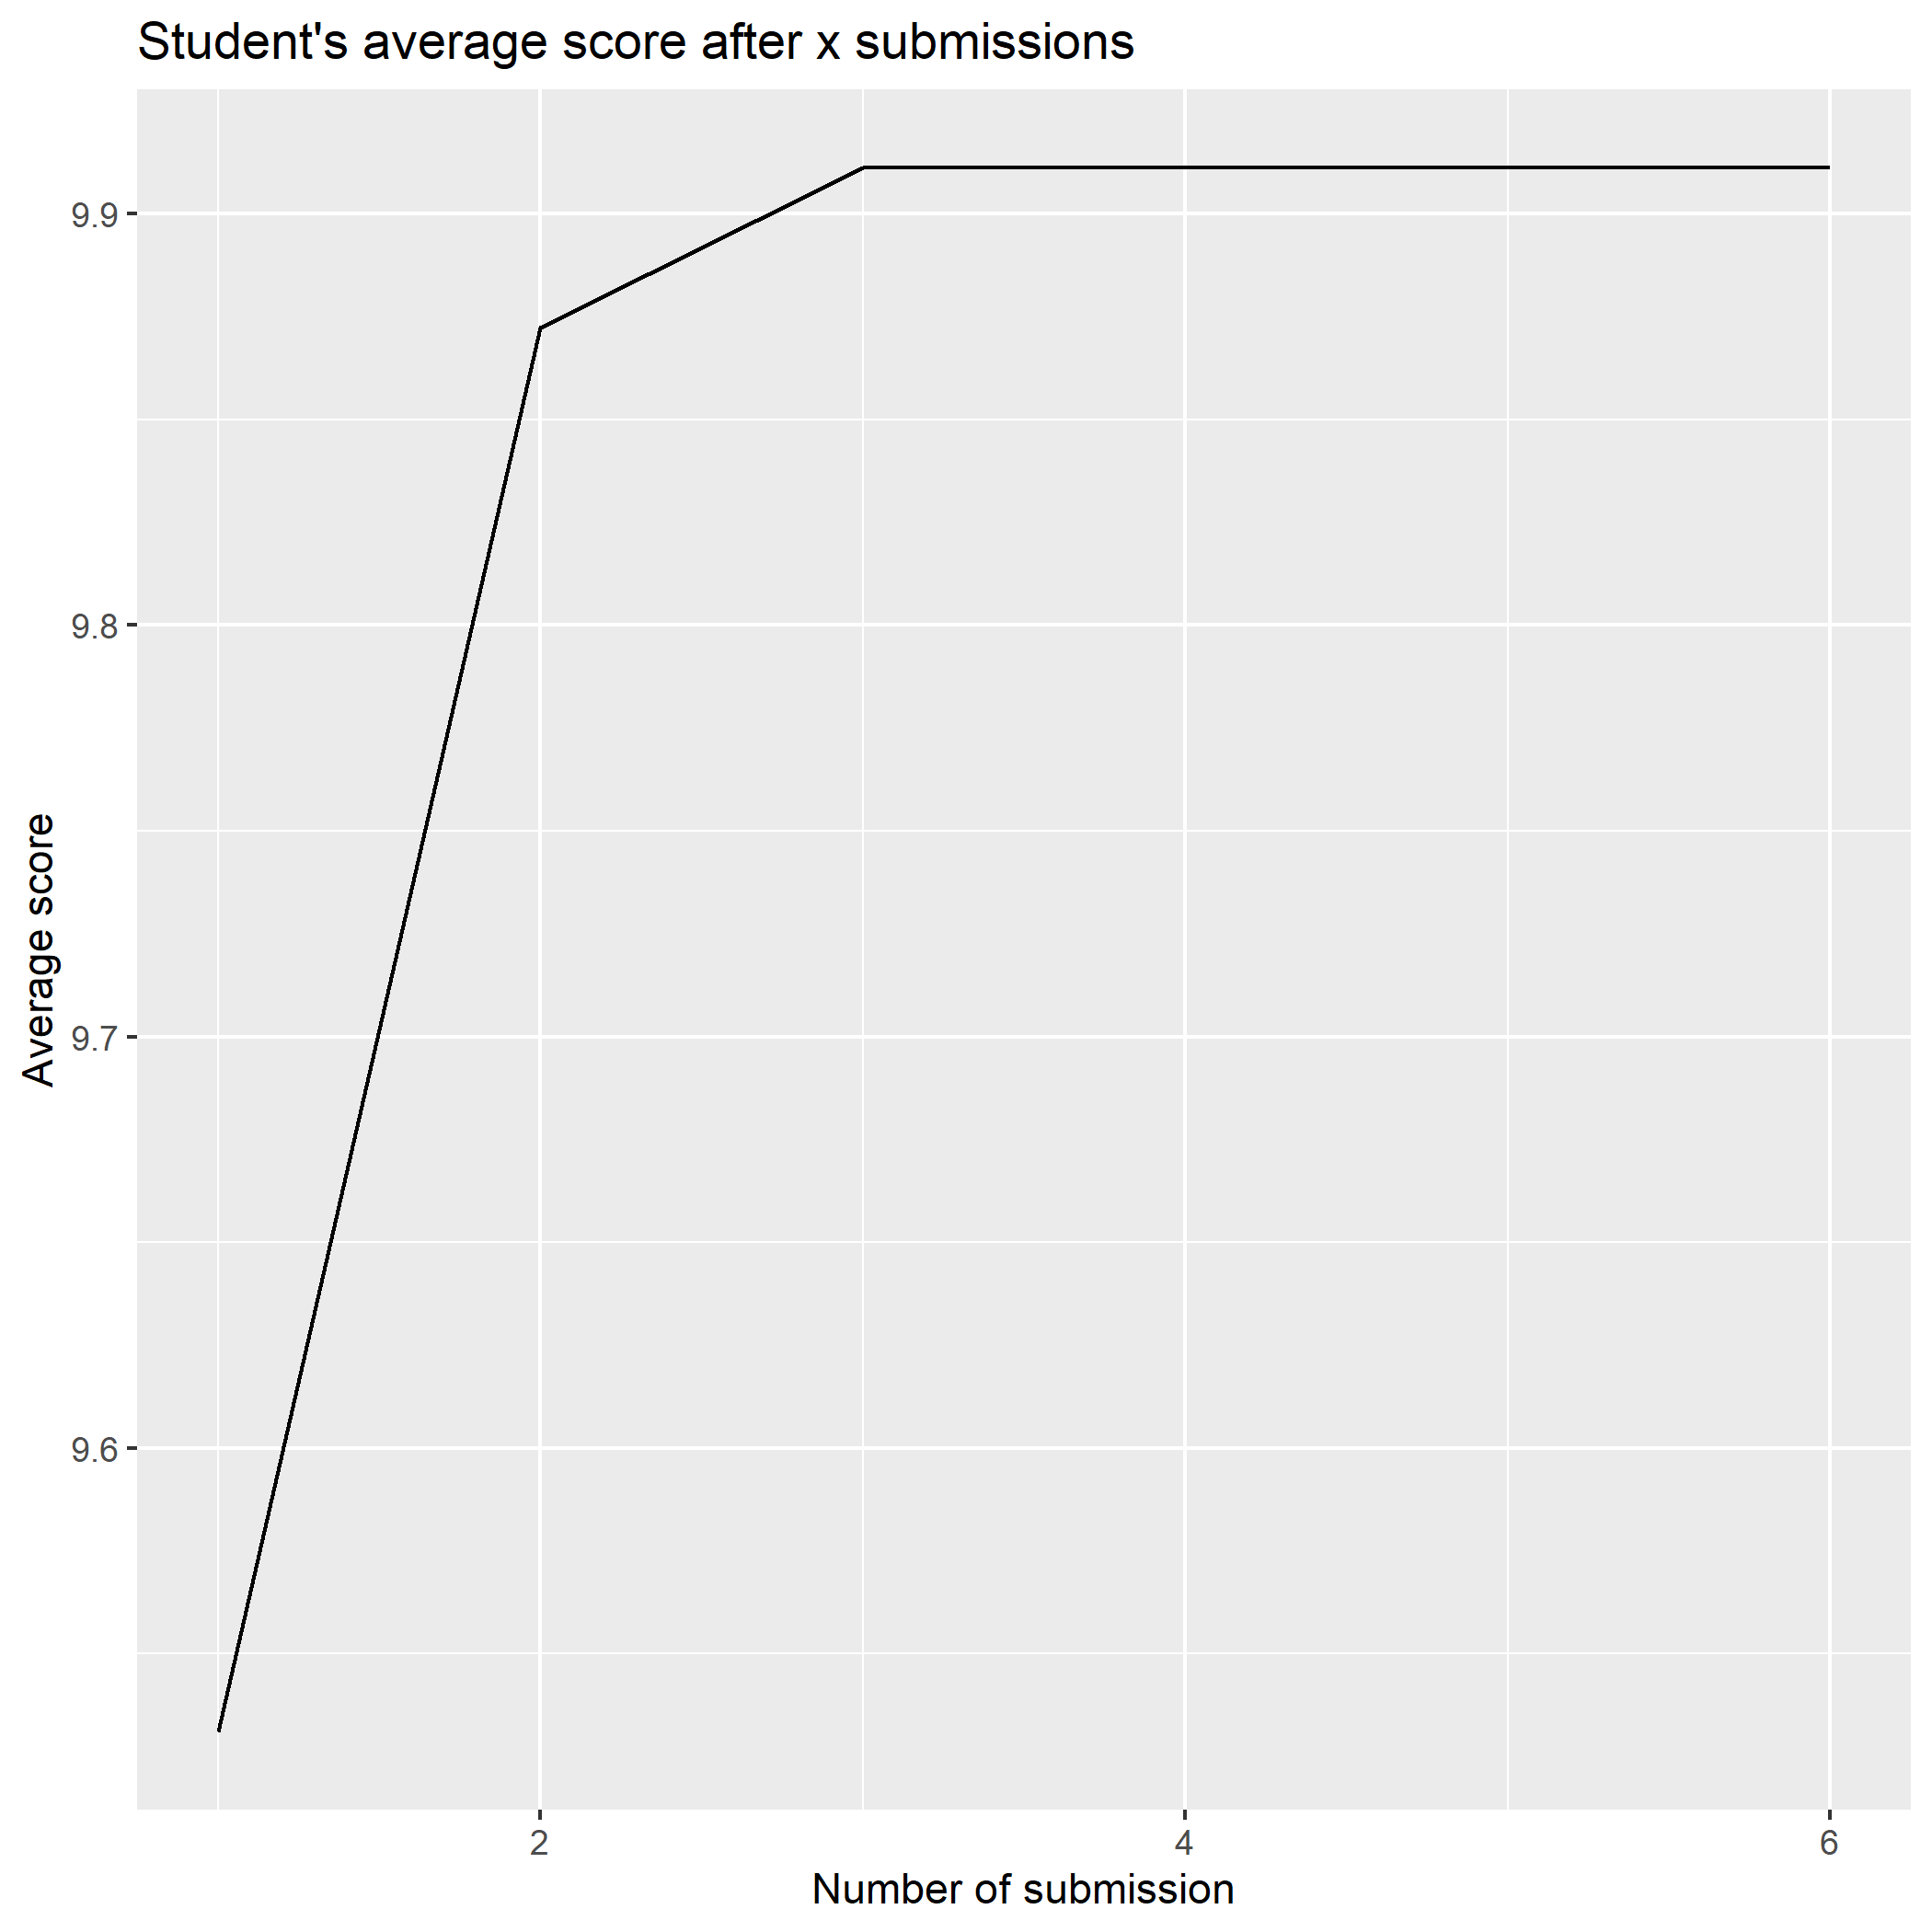
\includegraphics[scale=0.4]{Pics/q5c_file1.png}
    \caption{(5c) Điểm trung tất cả sinh viên tính theo sau k lần nộp}
    \label{fig:my_label}
\end{figure}

\newpage
\subsubsection{Câu 7}
\begin{figure}[!ht]
    \centering
    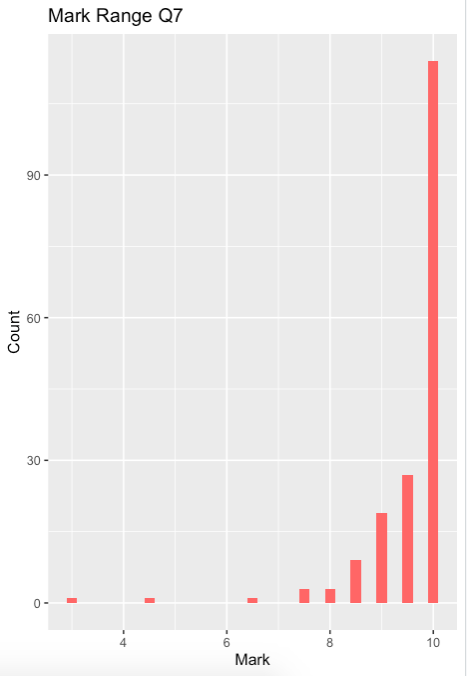
\includegraphics[scale=0.4]{Pics/q7-plot1.png}
    \caption{(7) Điểm trung tất cả sinh viên tính theo sau k lần nộp}
    \label{fig:my_label}
\end{figure}
\newpage
\subsubsection{Câu 9}
\begin{figure}[!ht]
    \centering
    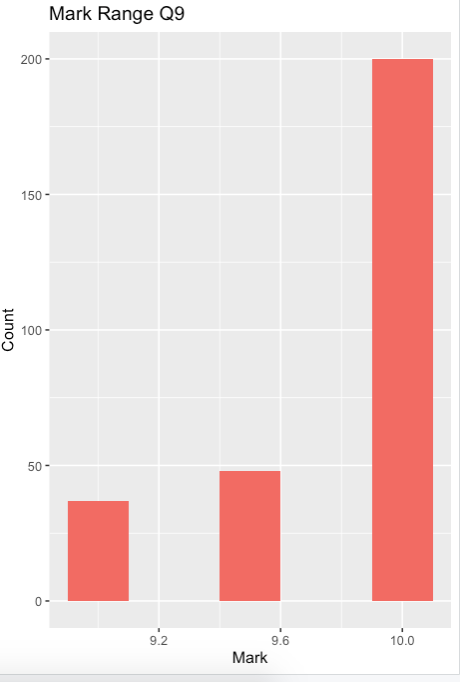
\includegraphics[scale=0.4]{Pics/q9-plot1.png}
    \caption{(9) Điểm trung tất cả sinh viên tính theo sau k lần nộp}
    \label{fig:my_label}
\end{figure}
\newpage
\subsubsection{Câu 10}
\newpage
\begin{figure}[!ht]
    \centering
    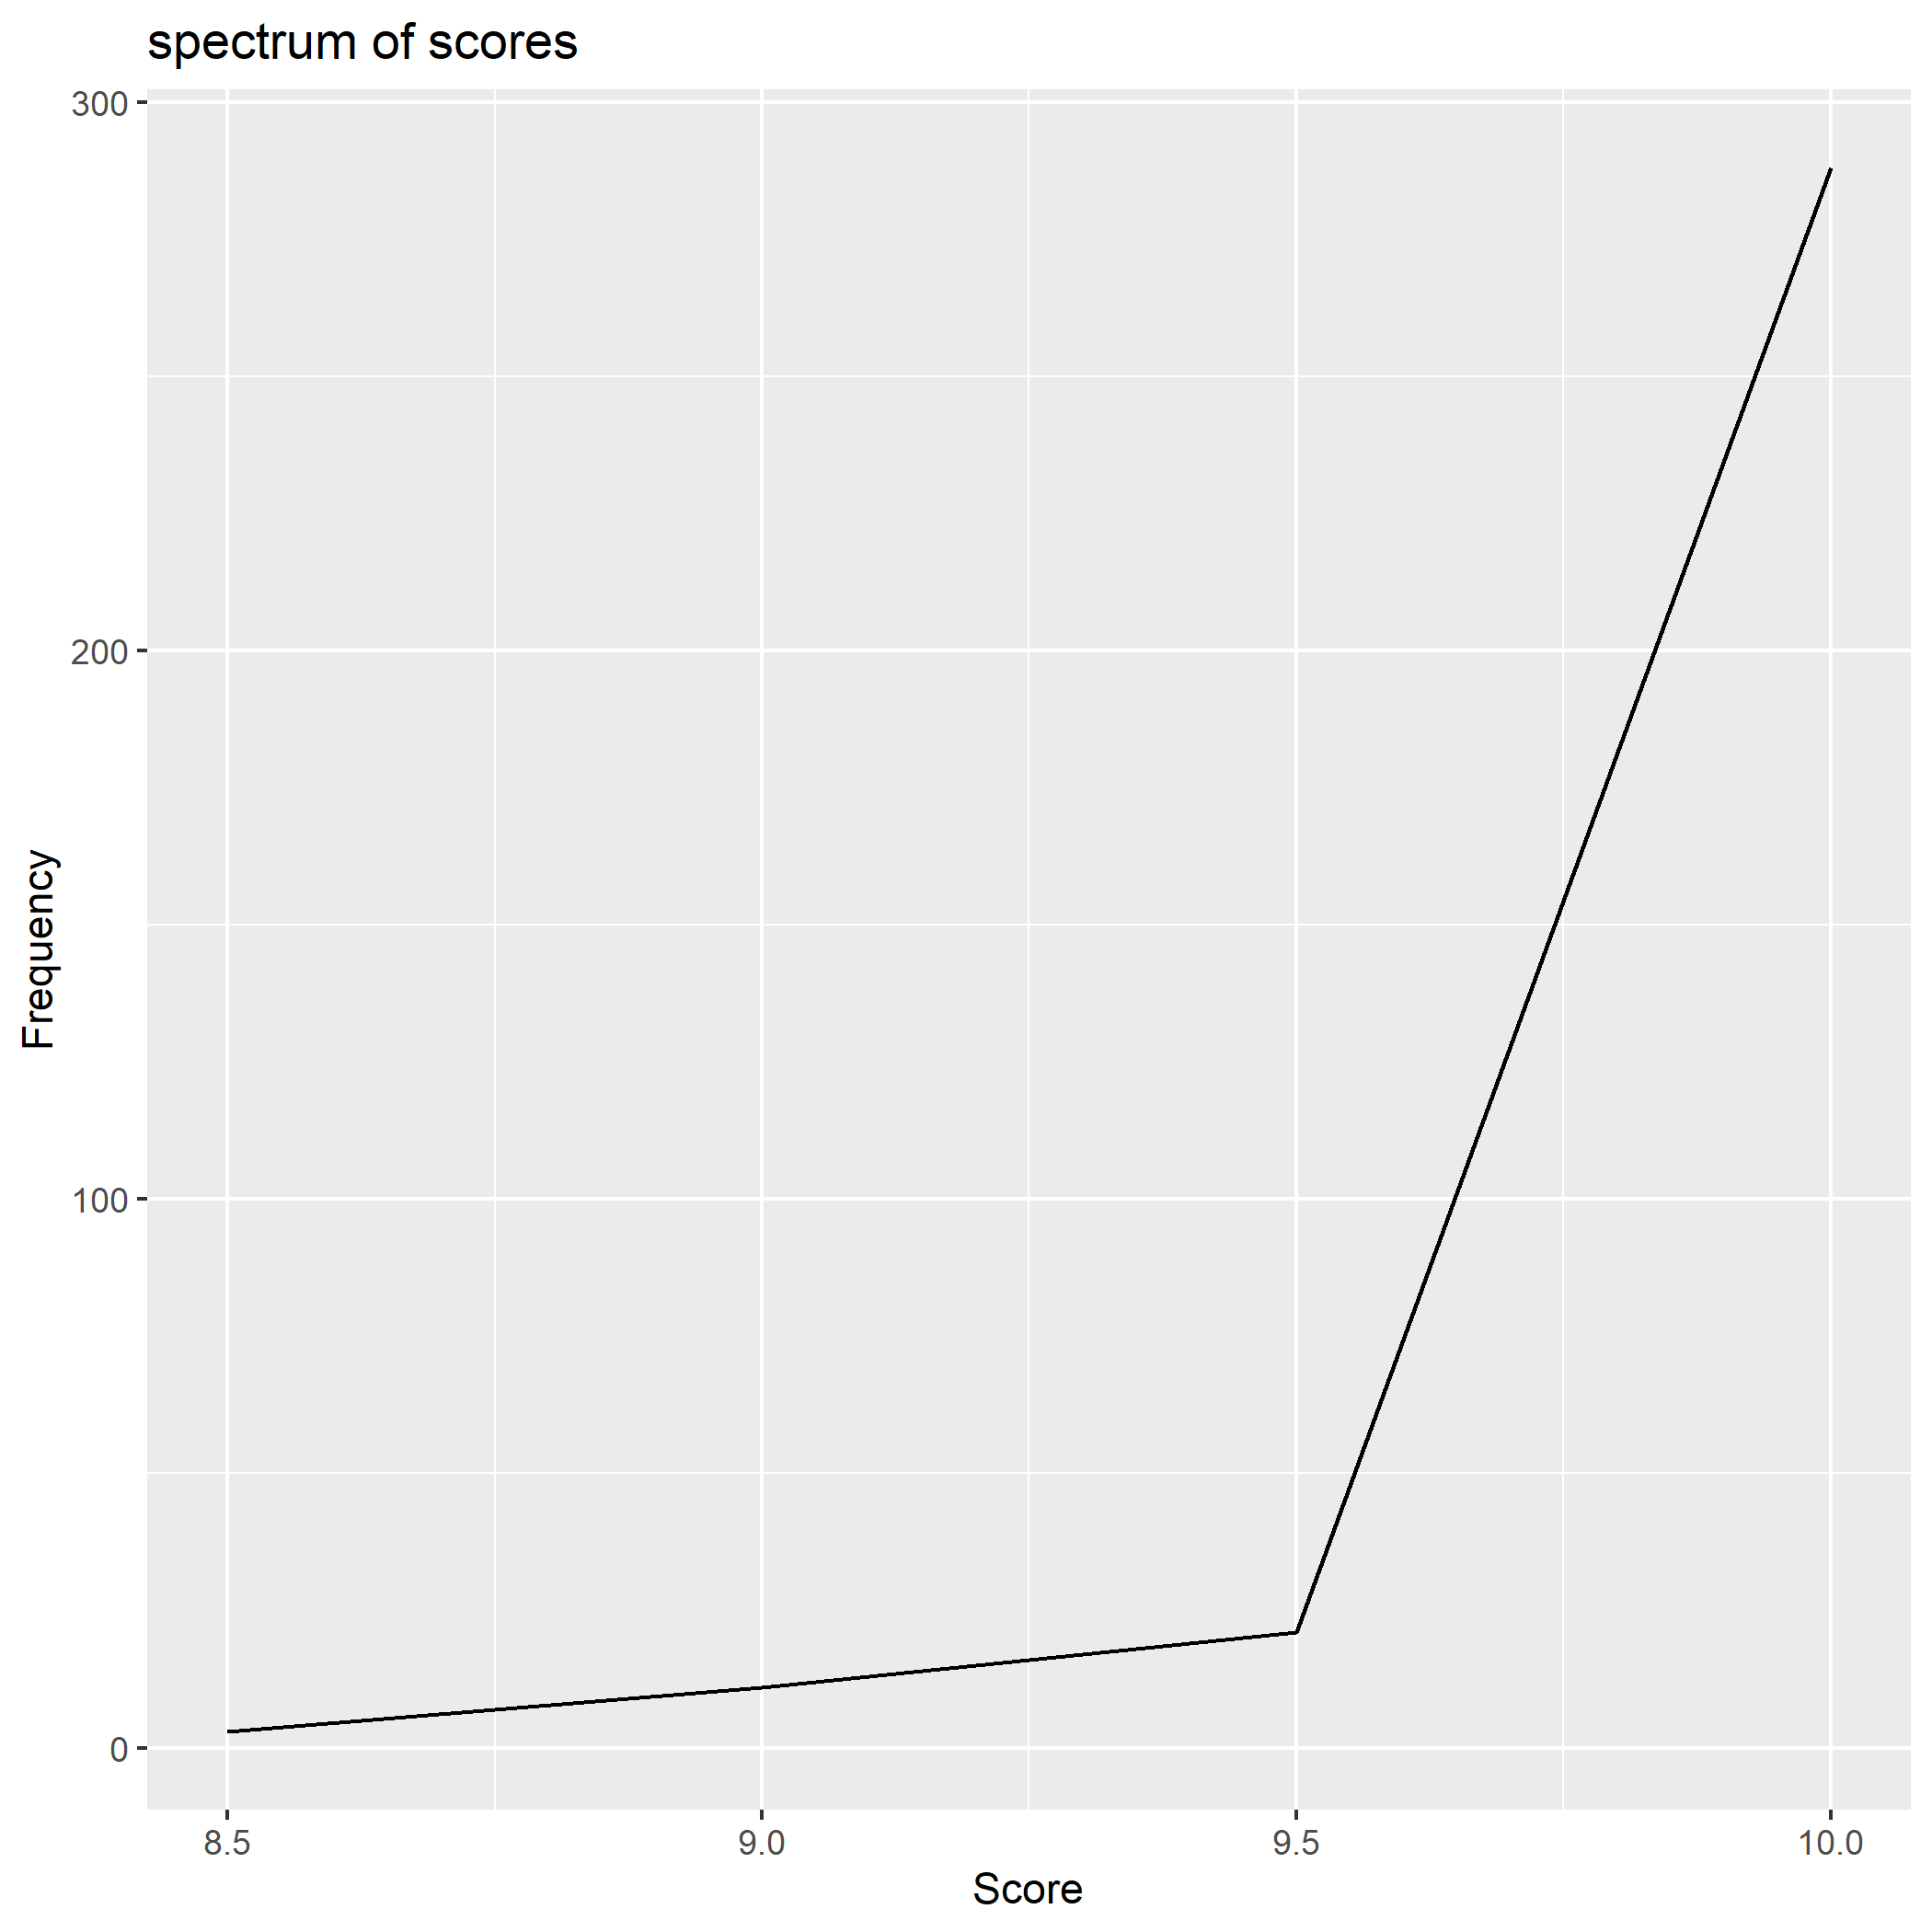
\includegraphics[scale=0.4]{Pics/q10c_file1.png}
    \caption{(10c) Phổ điểm sinh viên chủ động}
    \label{fig:my_label}
\end{figure}
\newpage
\subsubsection{Câu 11}

%%%%%%%%%%%%%%%%%%%%%%%%%%%%%%%%%%%%%%%%%%%%%%%%%%%
\newpage
\subsection{File 2}
\textbf{$tid = 11$}\\
Các kết quả không phải đồ thị được lưu vào file $2.tsv$. Các kết quả đồ thị được biểu diễn tại đây
\subsubsection{Câu 1}
\subsubsection{Câu 2}
\begin{figure}[!ht]
    \centering
    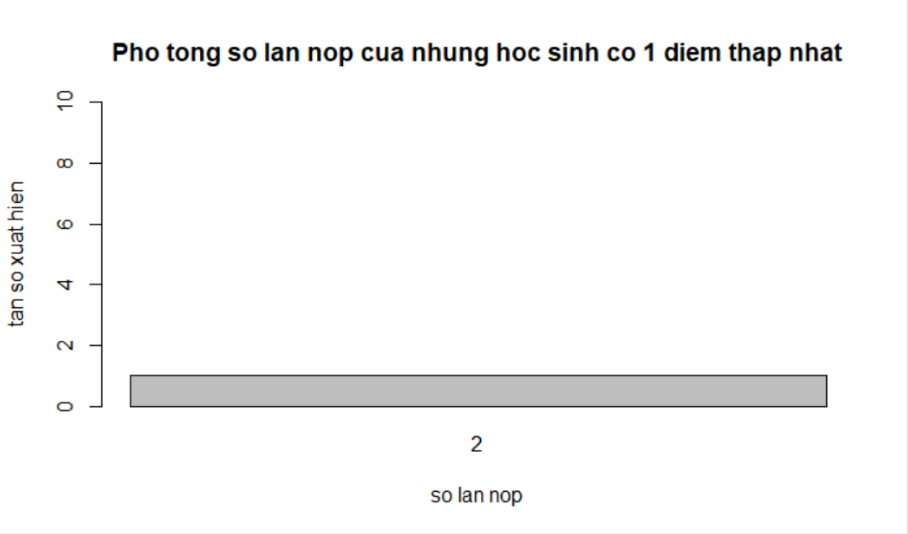
\includegraphics[scale=0.4]{Pics/q2d-file2.PNG}
    \caption{(2d) Phổ theo số lần nộp bài của sinh viên có ít nhất 1 bài nộp có điểm thấp nhất}
    \label{fig:my_label}
\end{figure}
\begin{figure}[!ht]
    \centering
    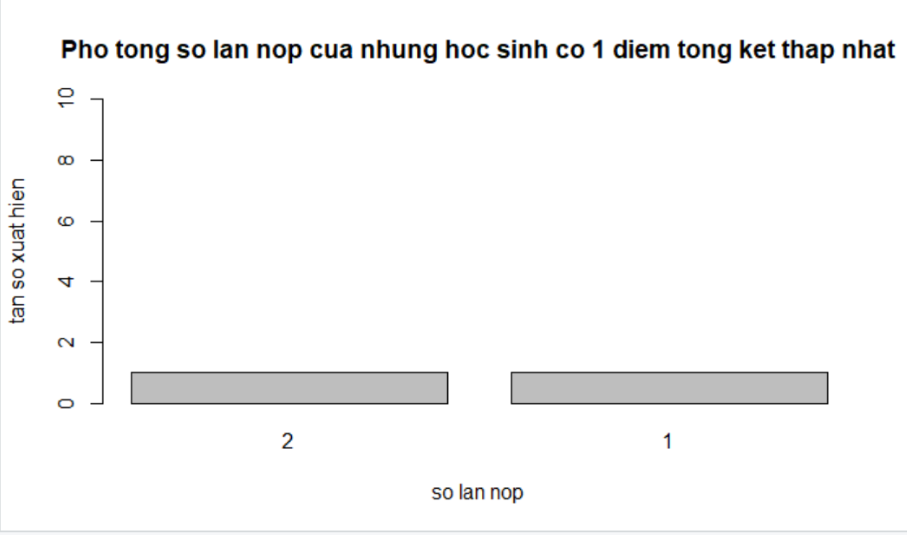
\includegraphics[scale=0.4]{Pics/q2g-file2.PNG}
    \caption{(2g) Phổ theo số lần nộp bài của các sinh viên có điểm số tổng kết thấp nhất }
    \label{fig:my_label}
\end{figure}
\newpage
\begin{figure}[!ht]
    \centering
    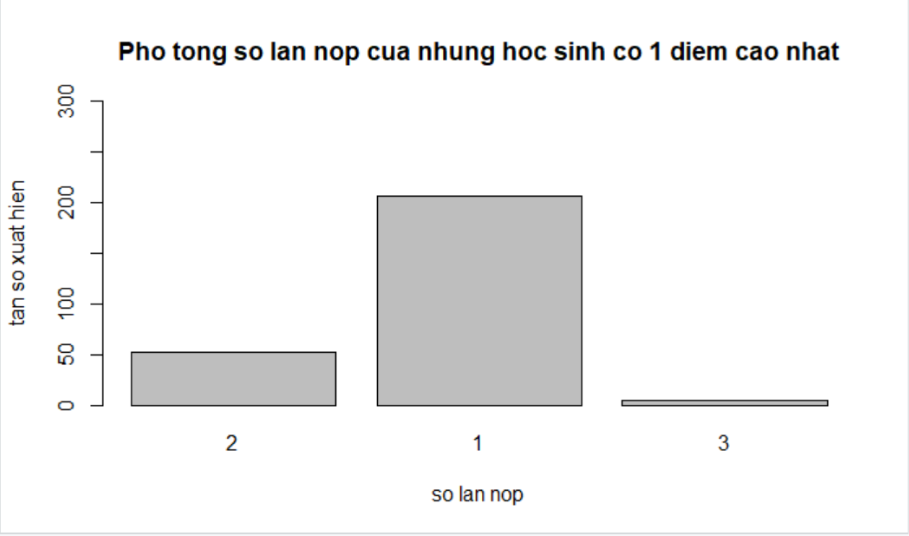
\includegraphics[scale=0.4]{Pics/q2j-file2.PNG}
    \caption{(2j)  Phổ theo số lần nộp bài của các sinh viên có tối thiểu một bài nộp có điểm số cao nhất}
    \label{fig:my_label}
\end{figure}
\begin{figure}[!ht]
    \centering
    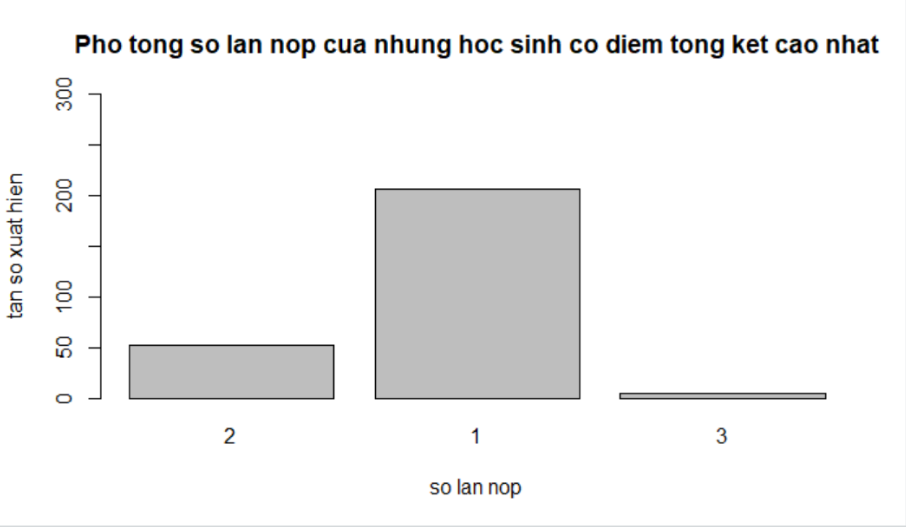
\includegraphics[scale=0.4]{Pics/q2m-file2.PNG}
    \caption{(2m) Phổ theo số lần nộp bài của các sinh viên có điểm số tổng kết cao nhấtn}
    \label{fig:my_label}
\end{figure}
\begin{figure}[!ht]
    \centering
    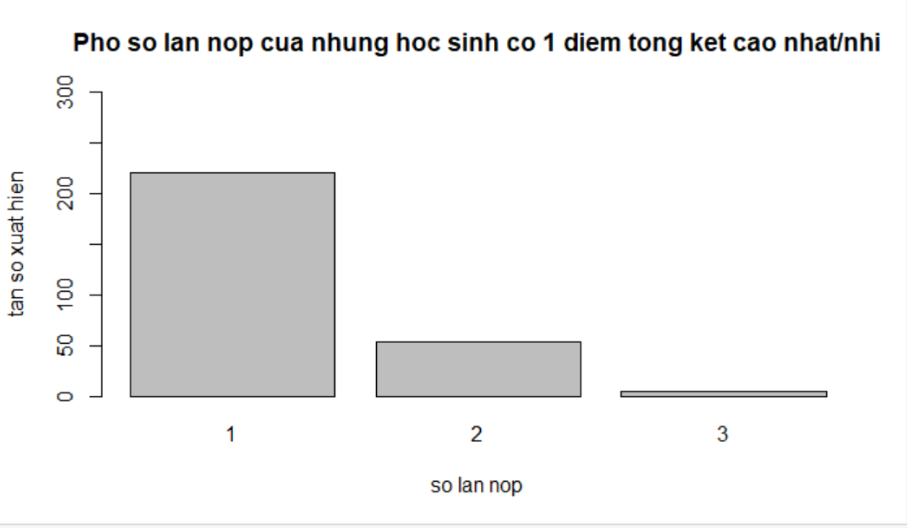
\includegraphics[scale=0.4]{Pics/q2u-file2.PNG}
    \caption{(2u) Phổ theo số lần nộp bài của các sinh viên có điểm số tổng kết ở 2 mức điểm cao nhất}
    \label{fig:my_label}
\end{figure}
\newpage 
\begin{figure}[!ht]
    \centering
    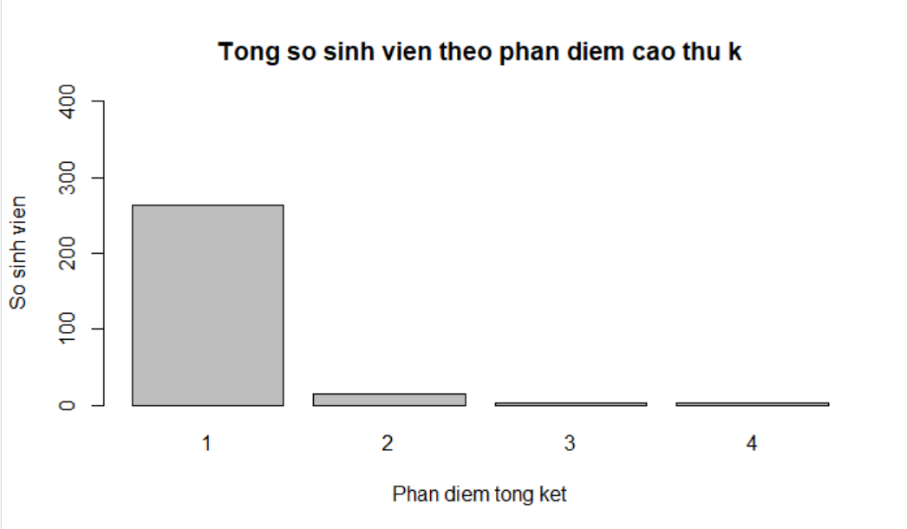
\includegraphics[scale=0.4]{Pics/q2v-file2.PNG}
    \caption{(2v) Số lượng sinh viên có điểm số tổng kết ở mức điểm cao thứ $k$ với $k$ cho trước}
    \label{fig:my_label}
\end{figure}
\newpage
\begin{figure}[!ht]
    \centering
    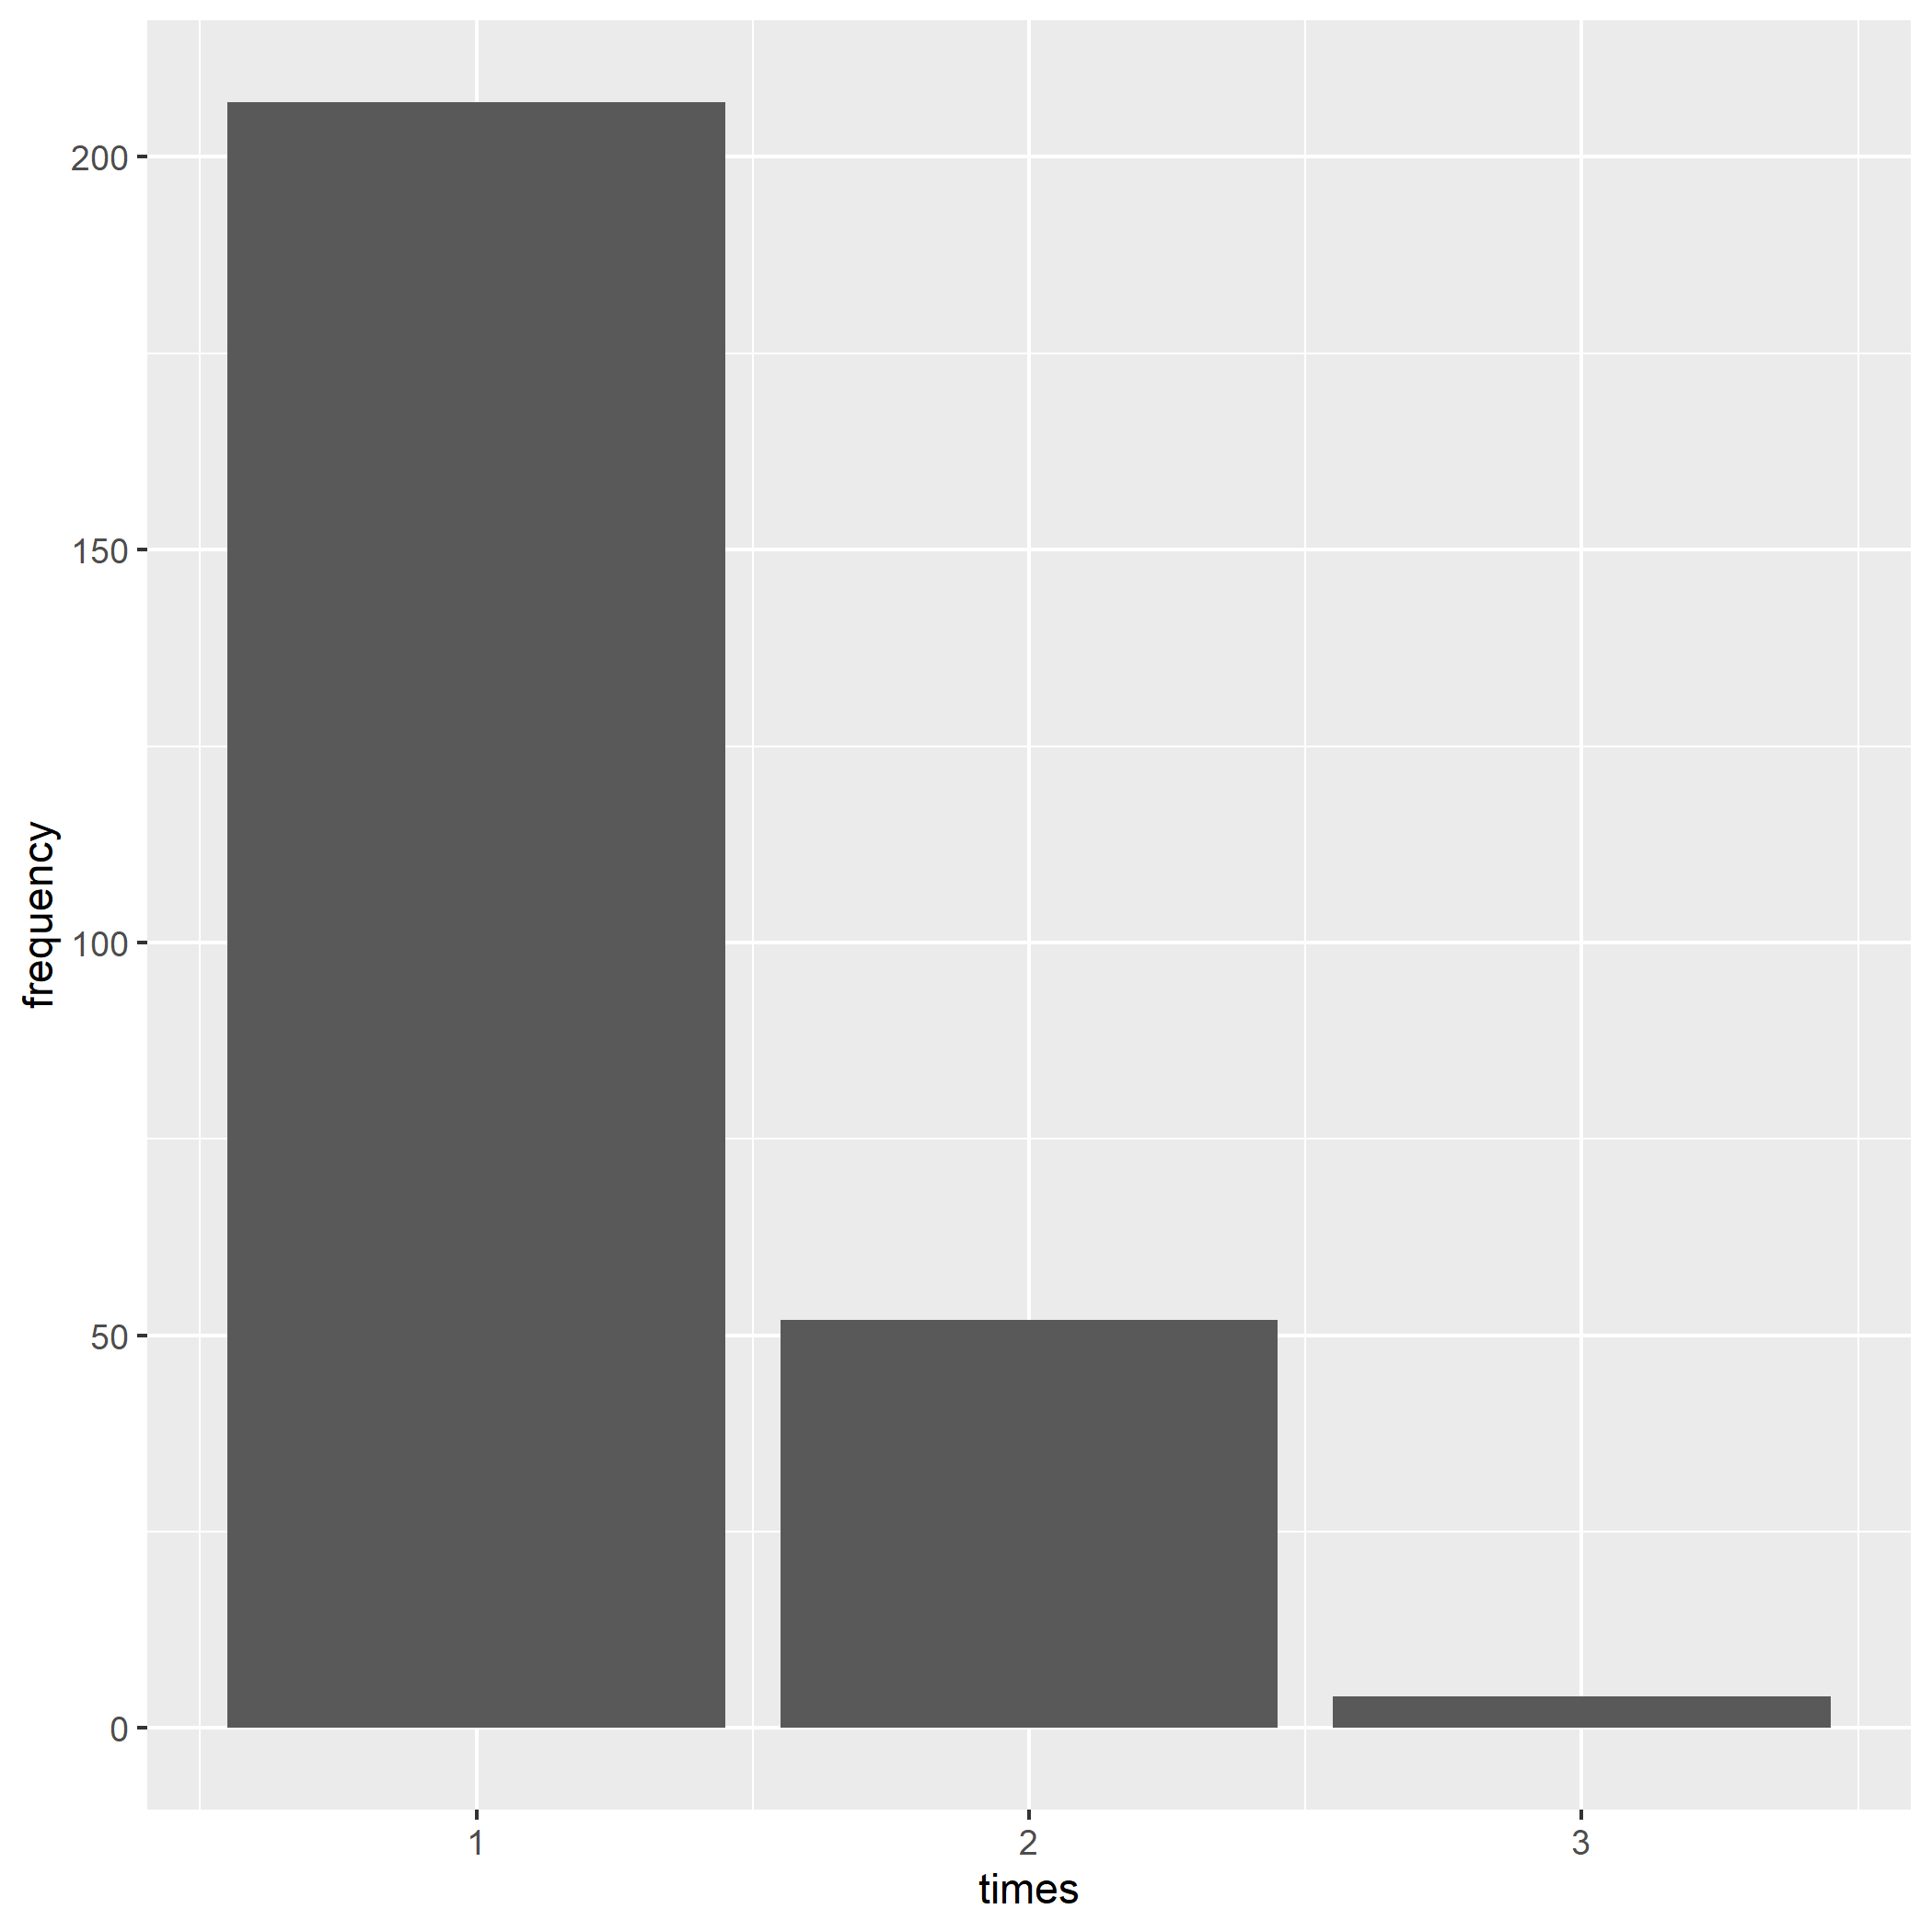
\includegraphics[scale=0.4]{Pics/q2w-1-file2.png}
    \caption{(2w) Phổ theo số lần nộp bài của các sinh viên có điểm số tổng kết ở mức điểm cao thứ $1$}
    \label{fig:my_label}
\end{figure}
\begin{figure}[!ht]
    \centering
    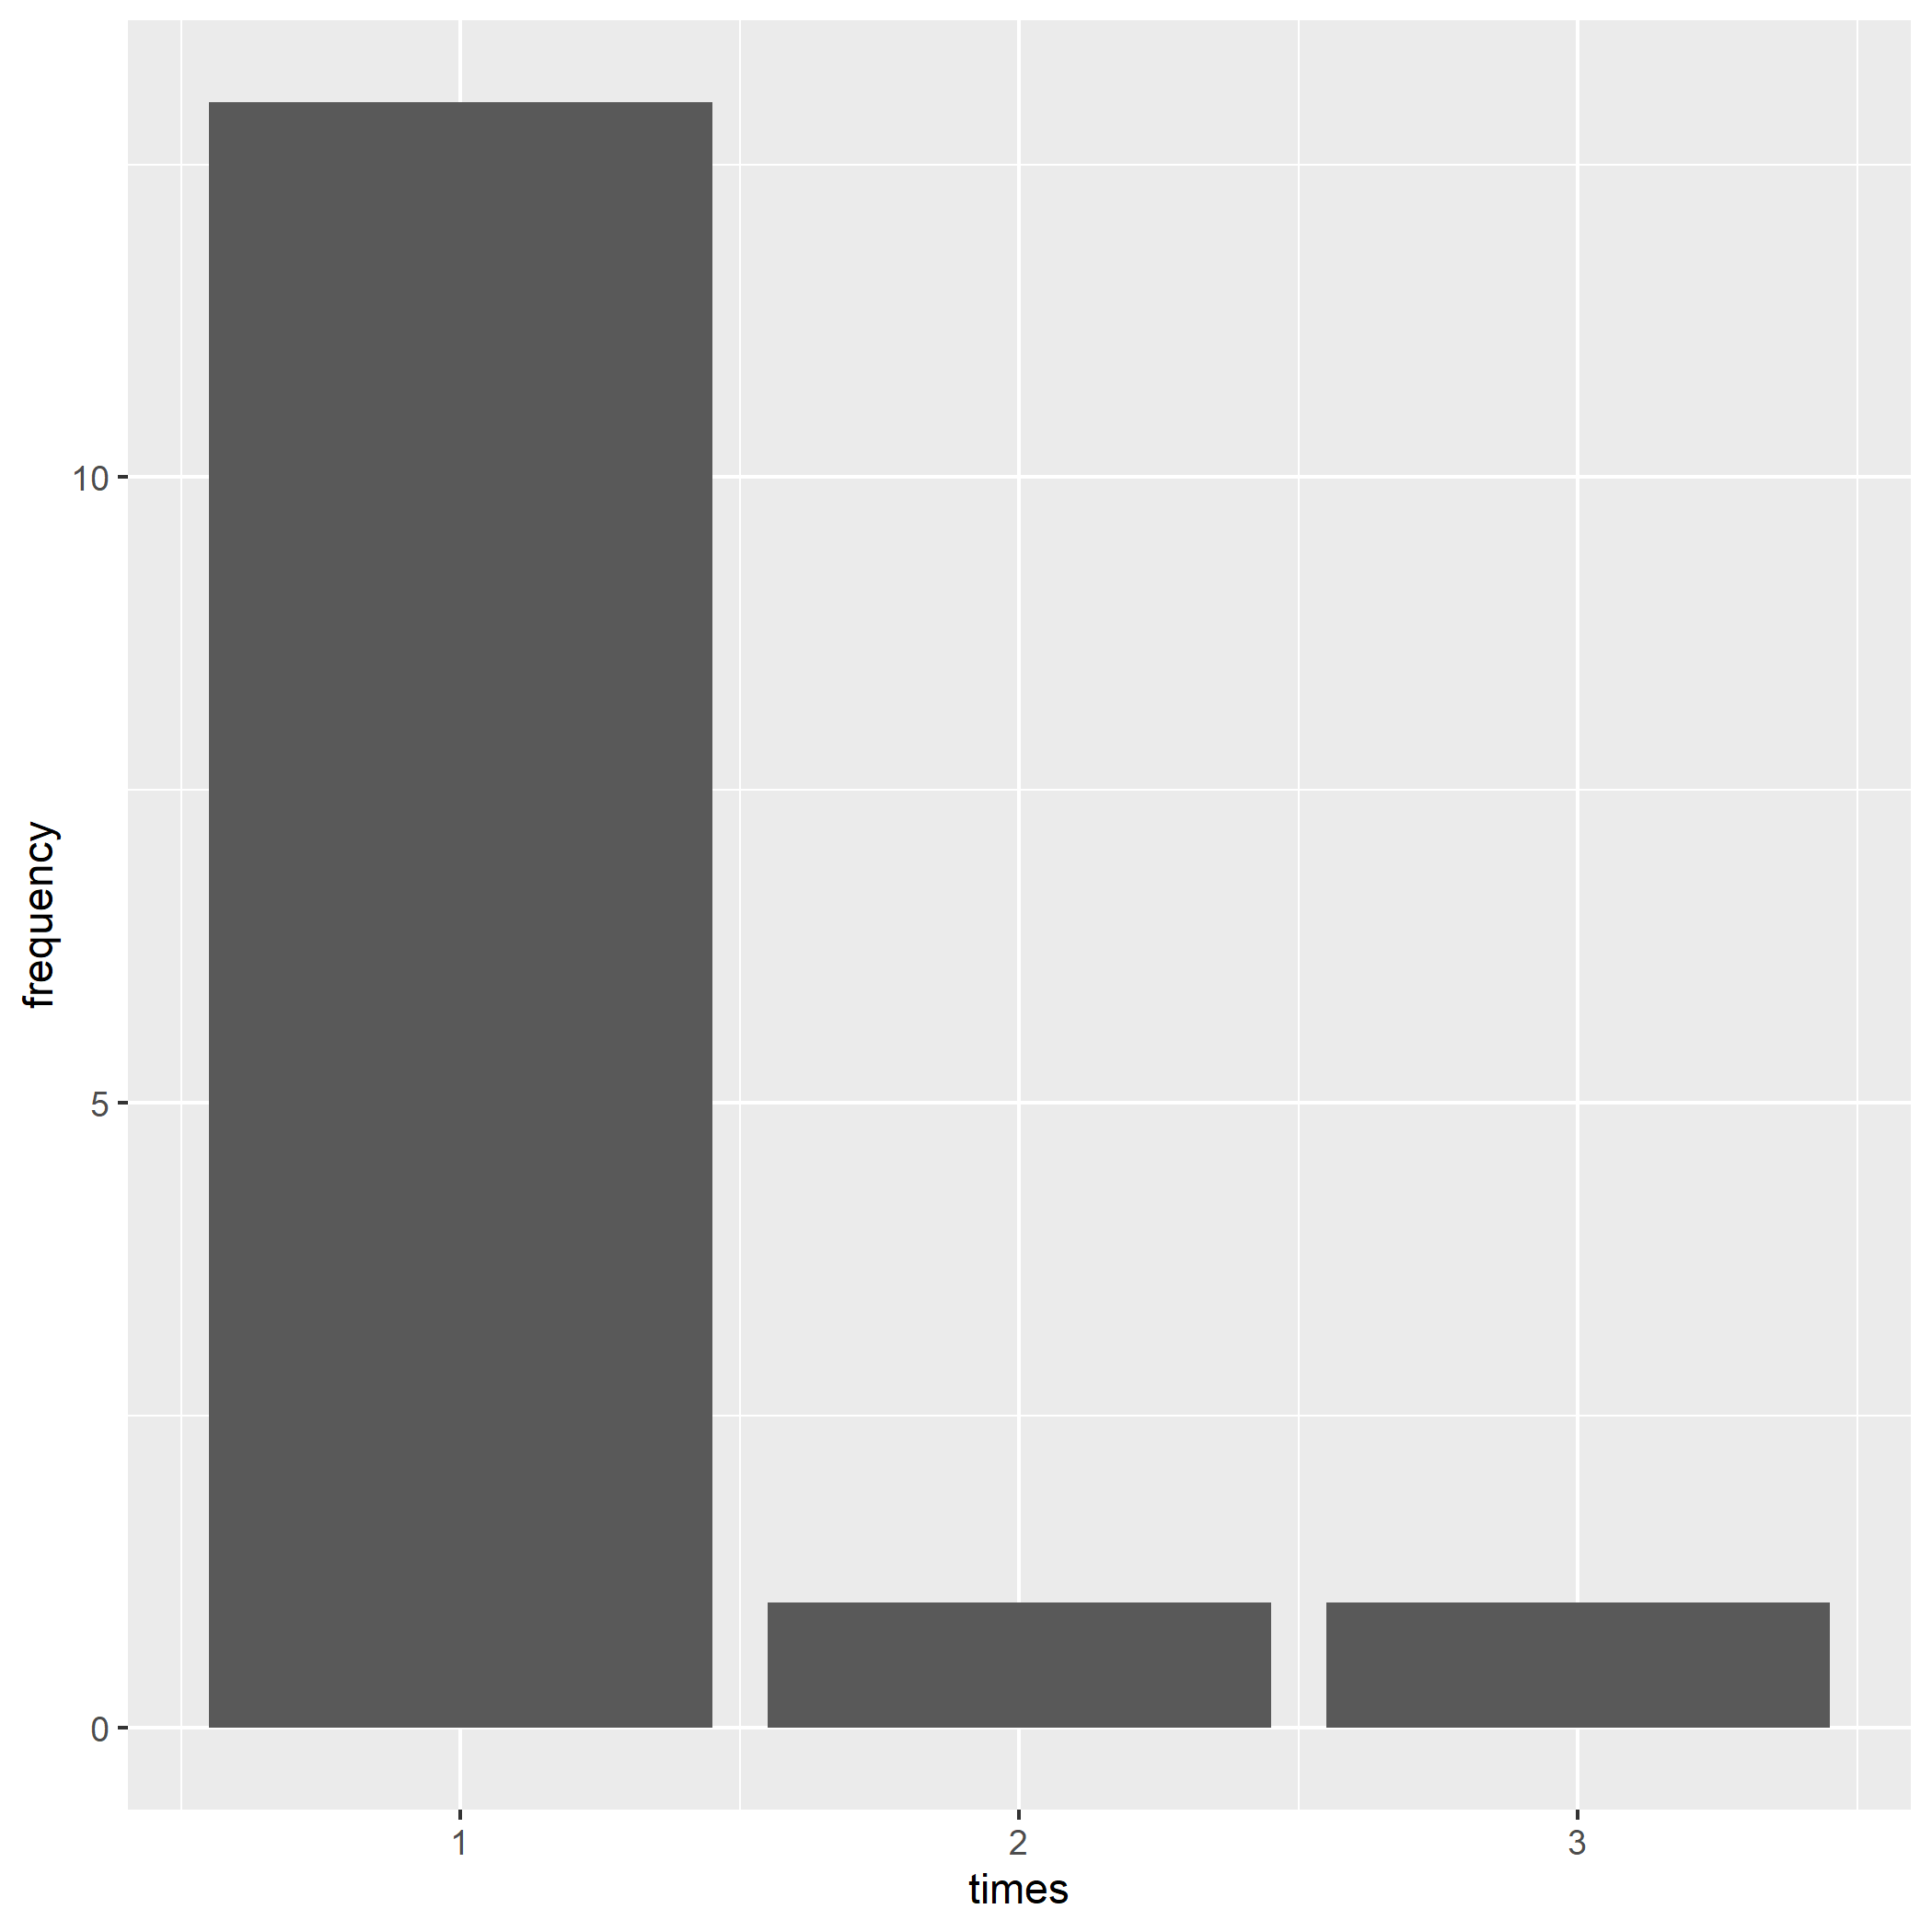
\includegraphics[scale=0.4]{Pics/q2w-2-file2.png}
    \caption{(2w) Phổ theo số lần nộp bài của các sinh viên có điểm số tổng kết ở mức điểm cao thứ $2$}
    \label{fig:my_label}
\end{figure}
\begin{figure}[!ht]
    \centering
    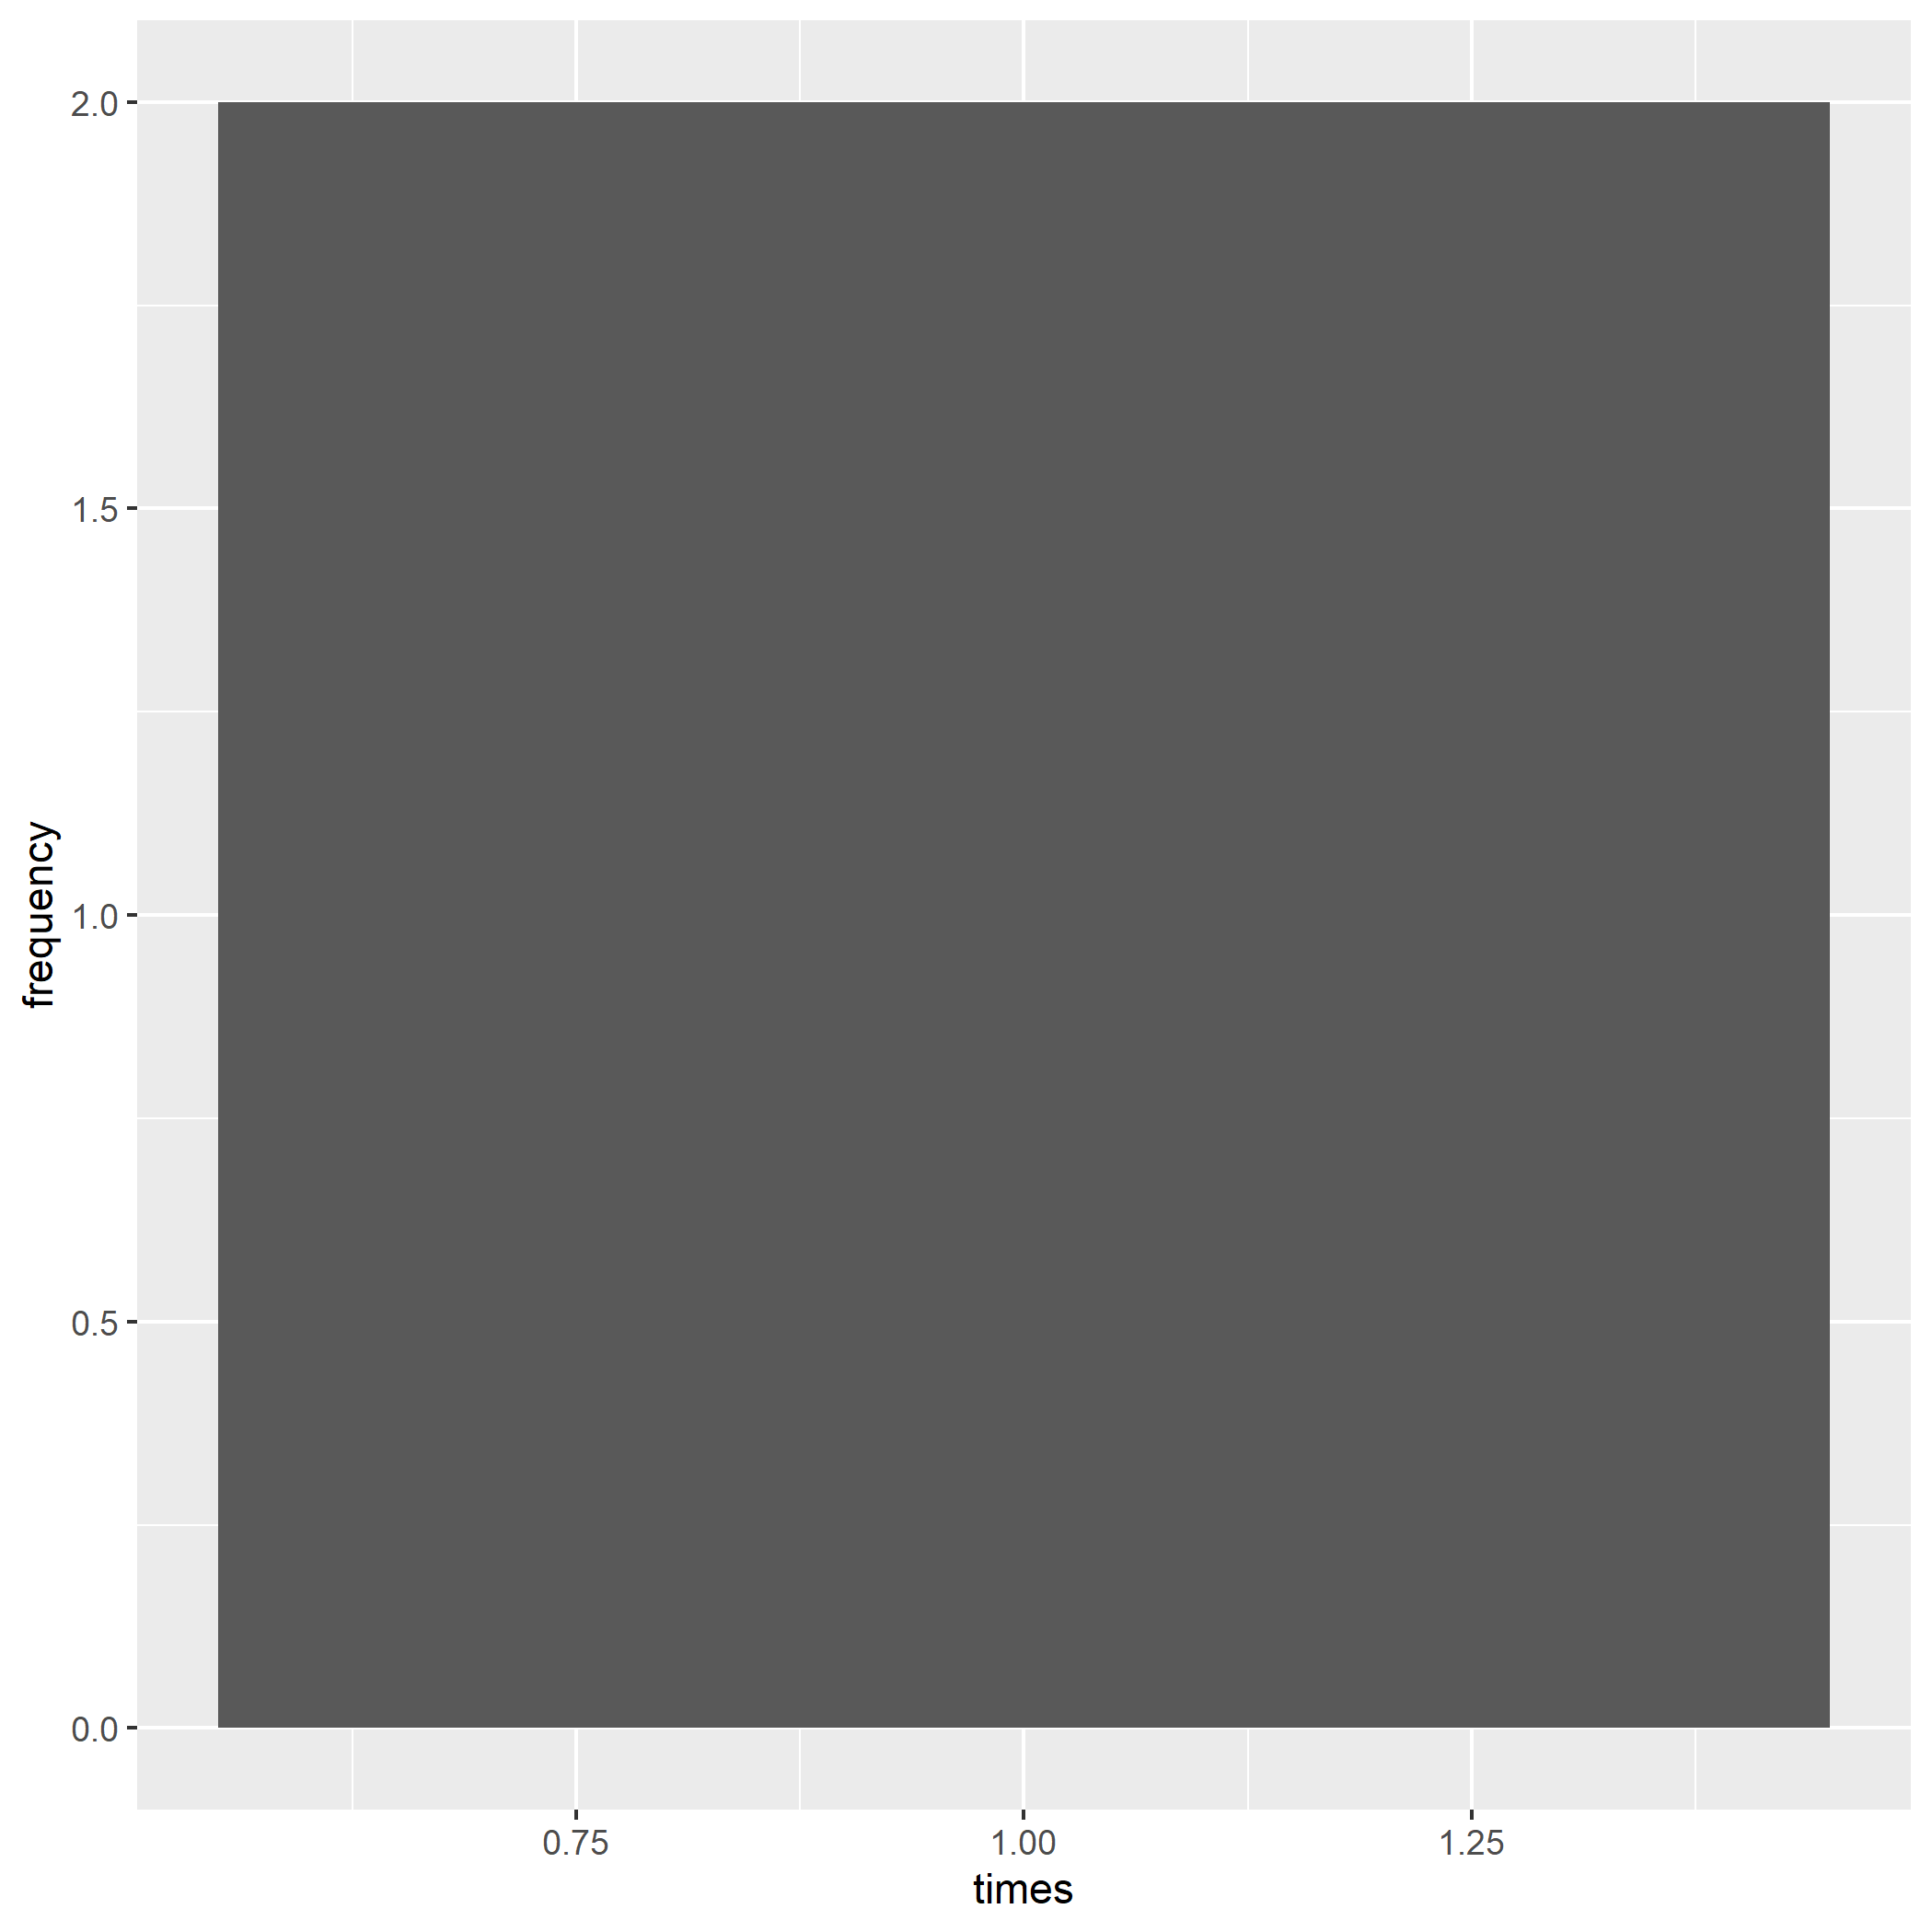
\includegraphics[scale=0.4]{Pics/q2w-3-file2.png}
    \caption{(2w) Phổ theo số lần nộp bài của các sinh viên có điểm số tổng kết ở mức điểm cao thứ $3$}
    \label{fig:my_label}
\end{figure}
\begin{figure}[!ht]
    \centering
    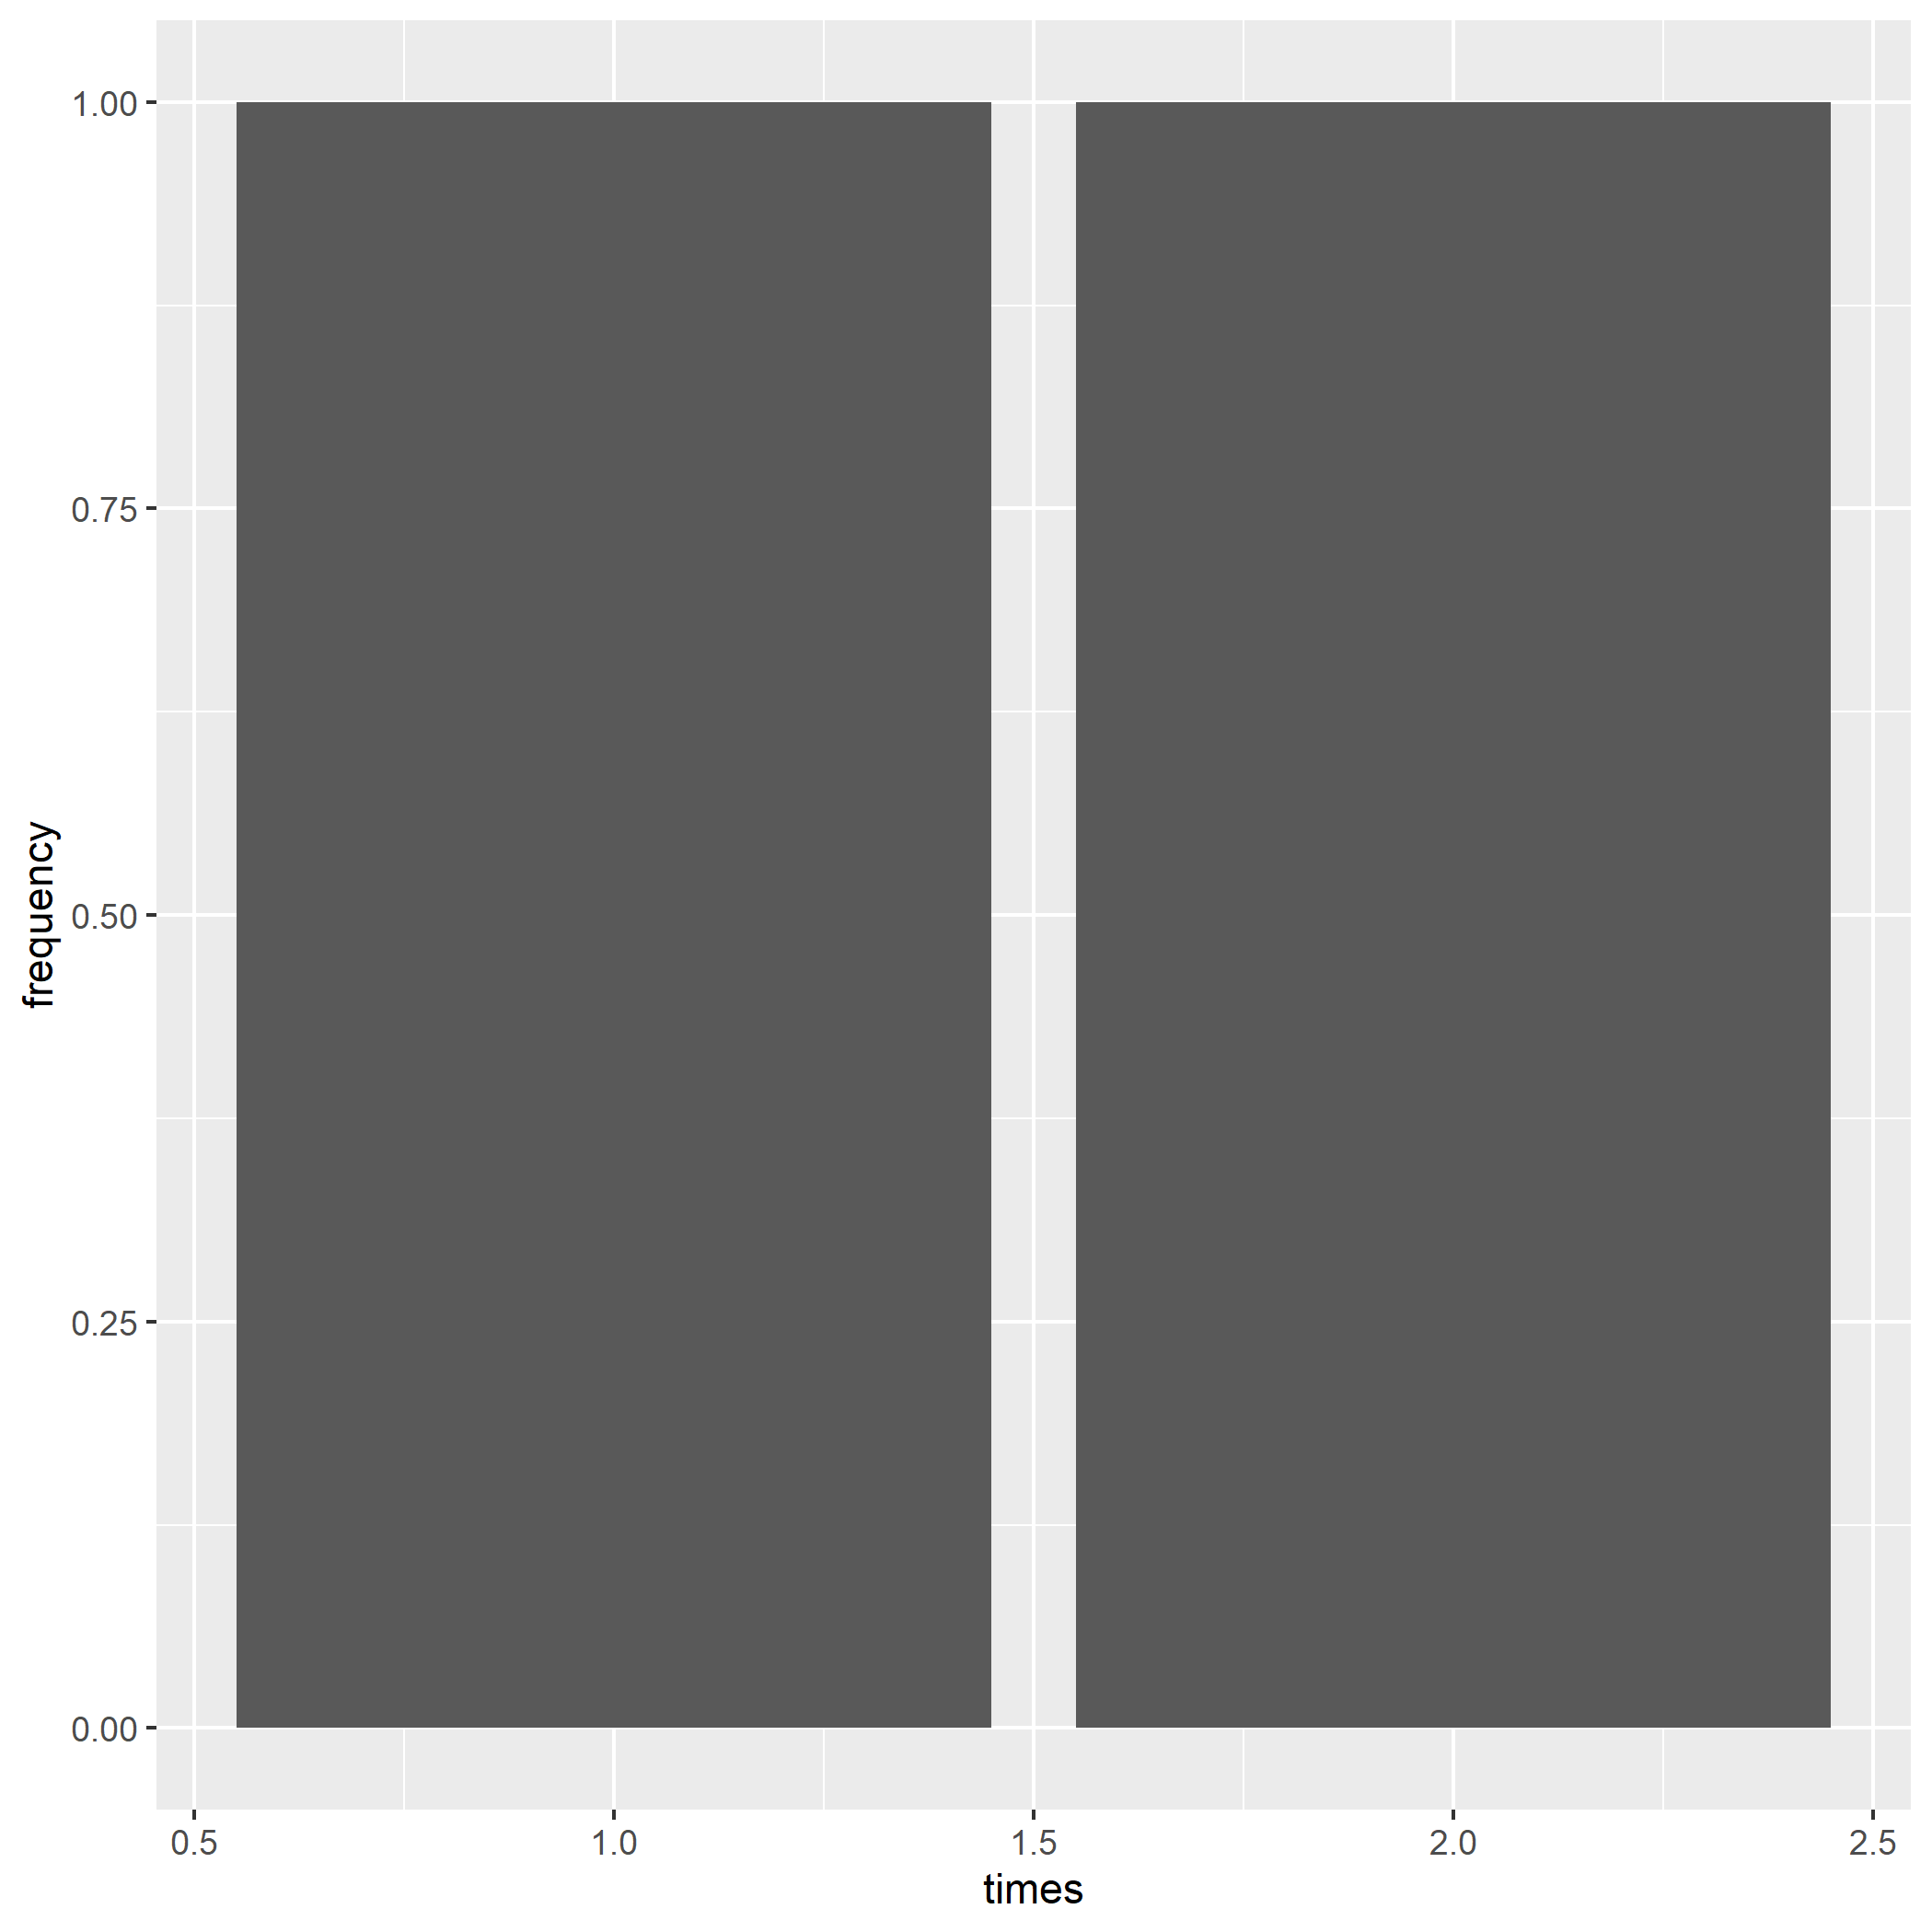
\includegraphics[scale=0.4]{Pics/q2w-4-file2.png}
    \caption{(2w) Phổ theo số lần nộp bài của các sinh viên có điểm số tổng kết ở mức điểm cao thứ $4$}
    \label{fig:my_label}
\end{figure}
\newpage
\subsubsection{Câu 3}
\subsubsection{Câu 4}
\begin{figure}[!ht]
    \centering
    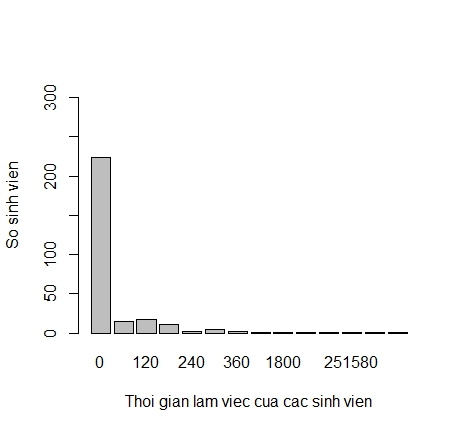
\includegraphics[scale=0.4]{Pics/q4b-file2.jpeg}
    \caption{(4b) Phổ thời gian làm việc (được tính từ lần nộp bài đầu tiên đến lần nộp cuối) của các
sinh viên.}
    \label{fig:my_label}
\end{figure}
\newpage
\begin{figure}[!ht]
    \centering
    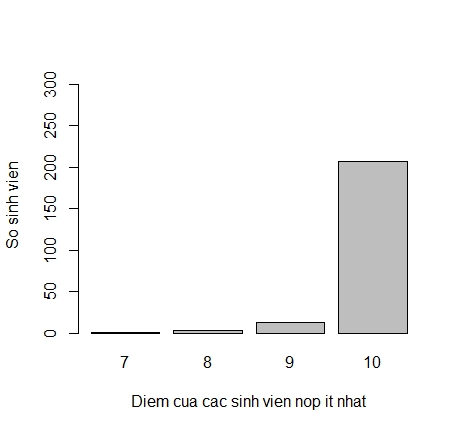
\includegraphics[scale=0.4]{Pics/q4e-file2.jpeg}
    \caption{(4e) Phổ điểm của các sinh viên có tần suất nộp bài ít nhất}
    \label{fig:my_label}
\end{figure}
\begin{figure}[!ht]
    \centering
    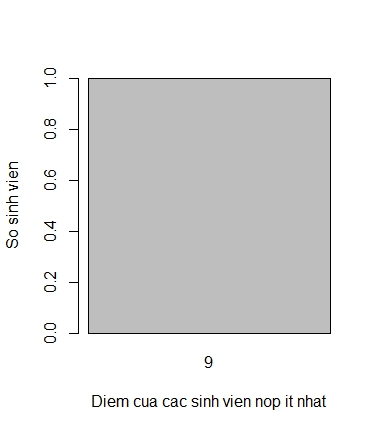
\includegraphics[scale=0.4]{Pics/q4h-file2.jpeg}
    \caption{(4h) Phổ điểm của các sinh viên có tần suất nộp bài nhiều nhất}
    \label{fig:my_label}
\end{figure}
\begin{figure}[!ht]
    \centering
    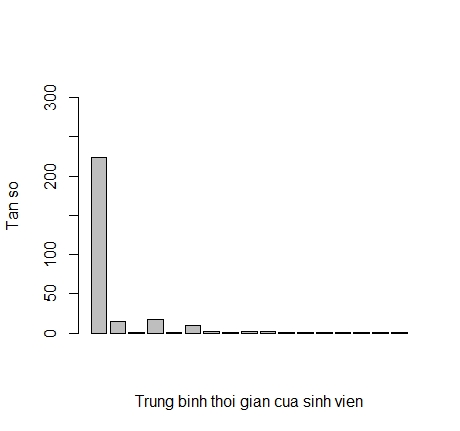
\includegraphics[scale=0.4]{Pics/q4m-file2.jpeg}
    \caption{(4m) Biểu đồ tần số của mẫu}
    \label{fig:my_label}
\end{figure}
\begin{figure}[!ht]
    \centering
    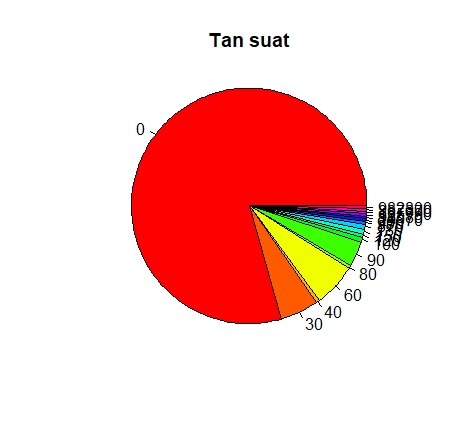
\includegraphics[scale=0.4]{Pics/q4n-file2.jpeg}
    \caption{(4n) Biểu đồ tần suất của mẫu}
    \label{fig:my_label}
\end{figure}
\newpage
\begin{figure}[!ht]
    \centering
    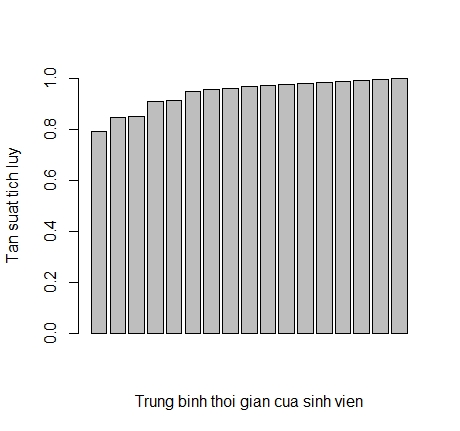
\includegraphics[scale=0.4]{Pics/q4o-file2.jpeg}
    \caption{(4o) Biểu đồ tần suất tích lũy của mẫu }
    \label{fig:my_label}
\end{figure}
\subsubsection{Câu 5}
\begin{figure}[!ht]
    \centering
    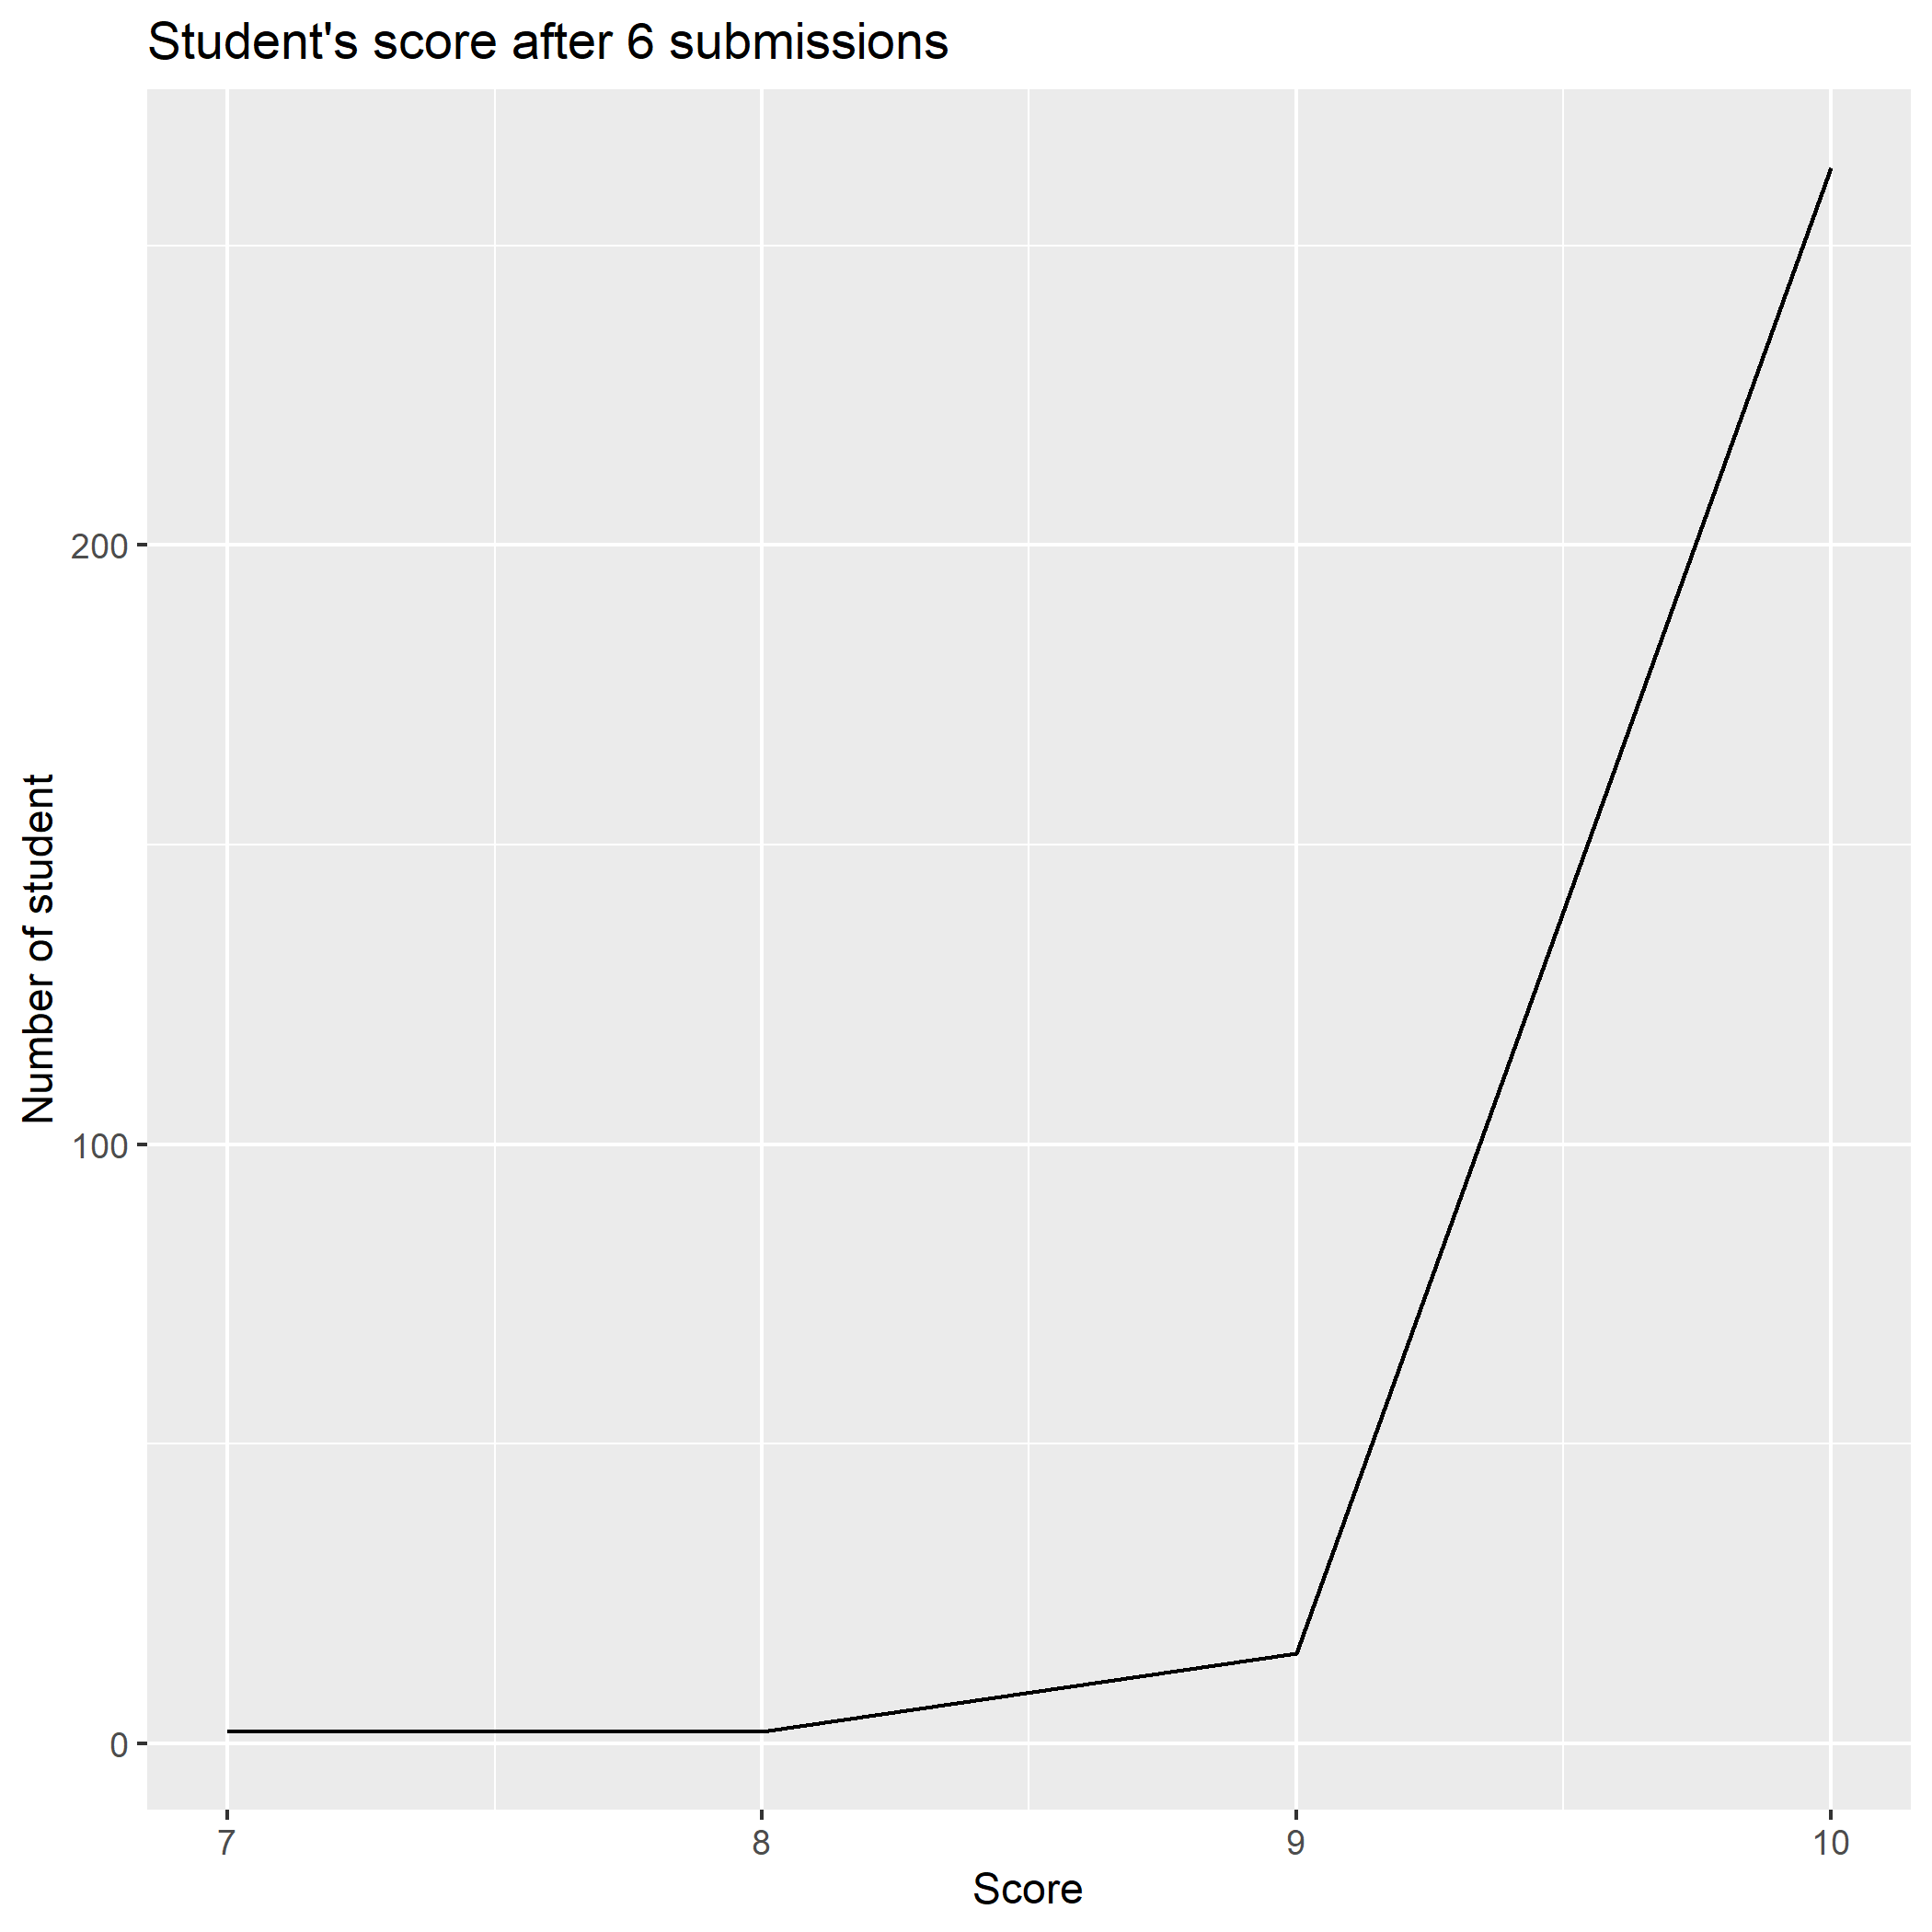
\includegraphics[scale=0.4]{Pics/q5a_file2.png}
    \caption{(5a) Điểm sinh viên sau 6 lần nộp}
    \label{fig:my_label}
\end{figure}
\begin{figure}[!ht]
    \centering
    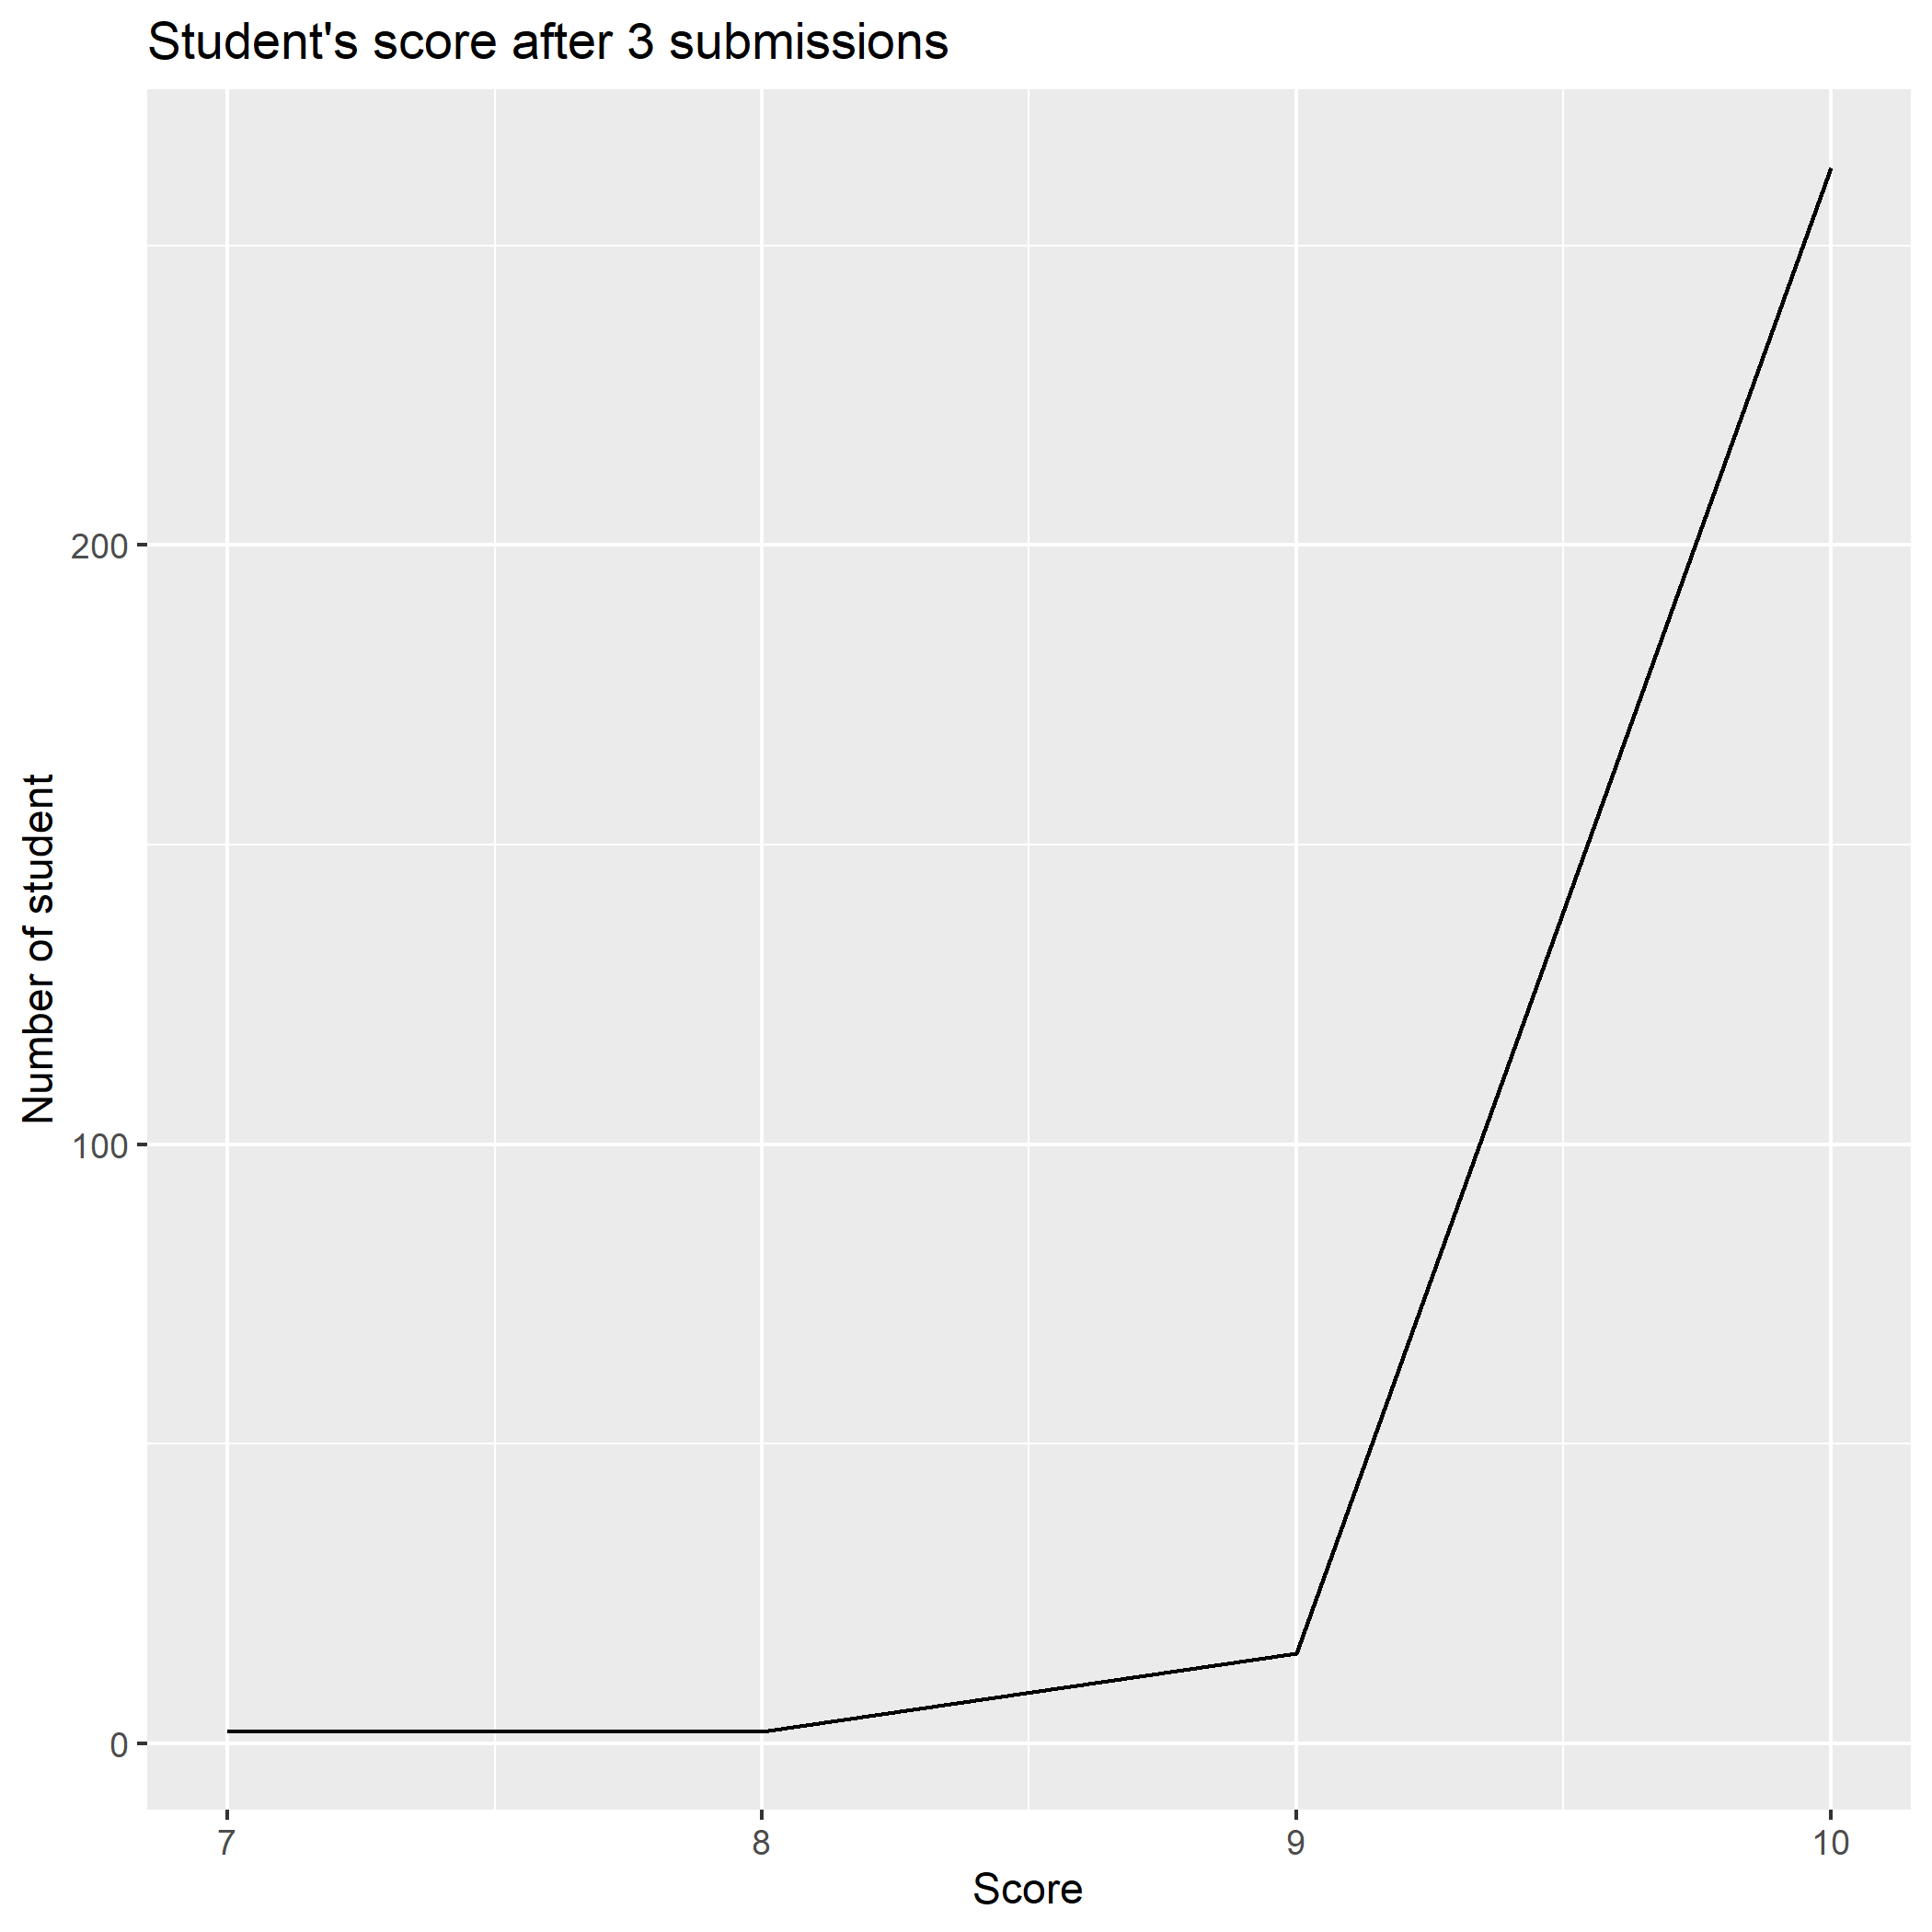
\includegraphics[scale=0.4]{Pics/q5b_file2.png}
    \caption{(5b) Điểm sinh viên sau 3 lần nộp}
    \label{fig:my_label}
\end{figure}
\begin{figure}[!ht]
    \centering
    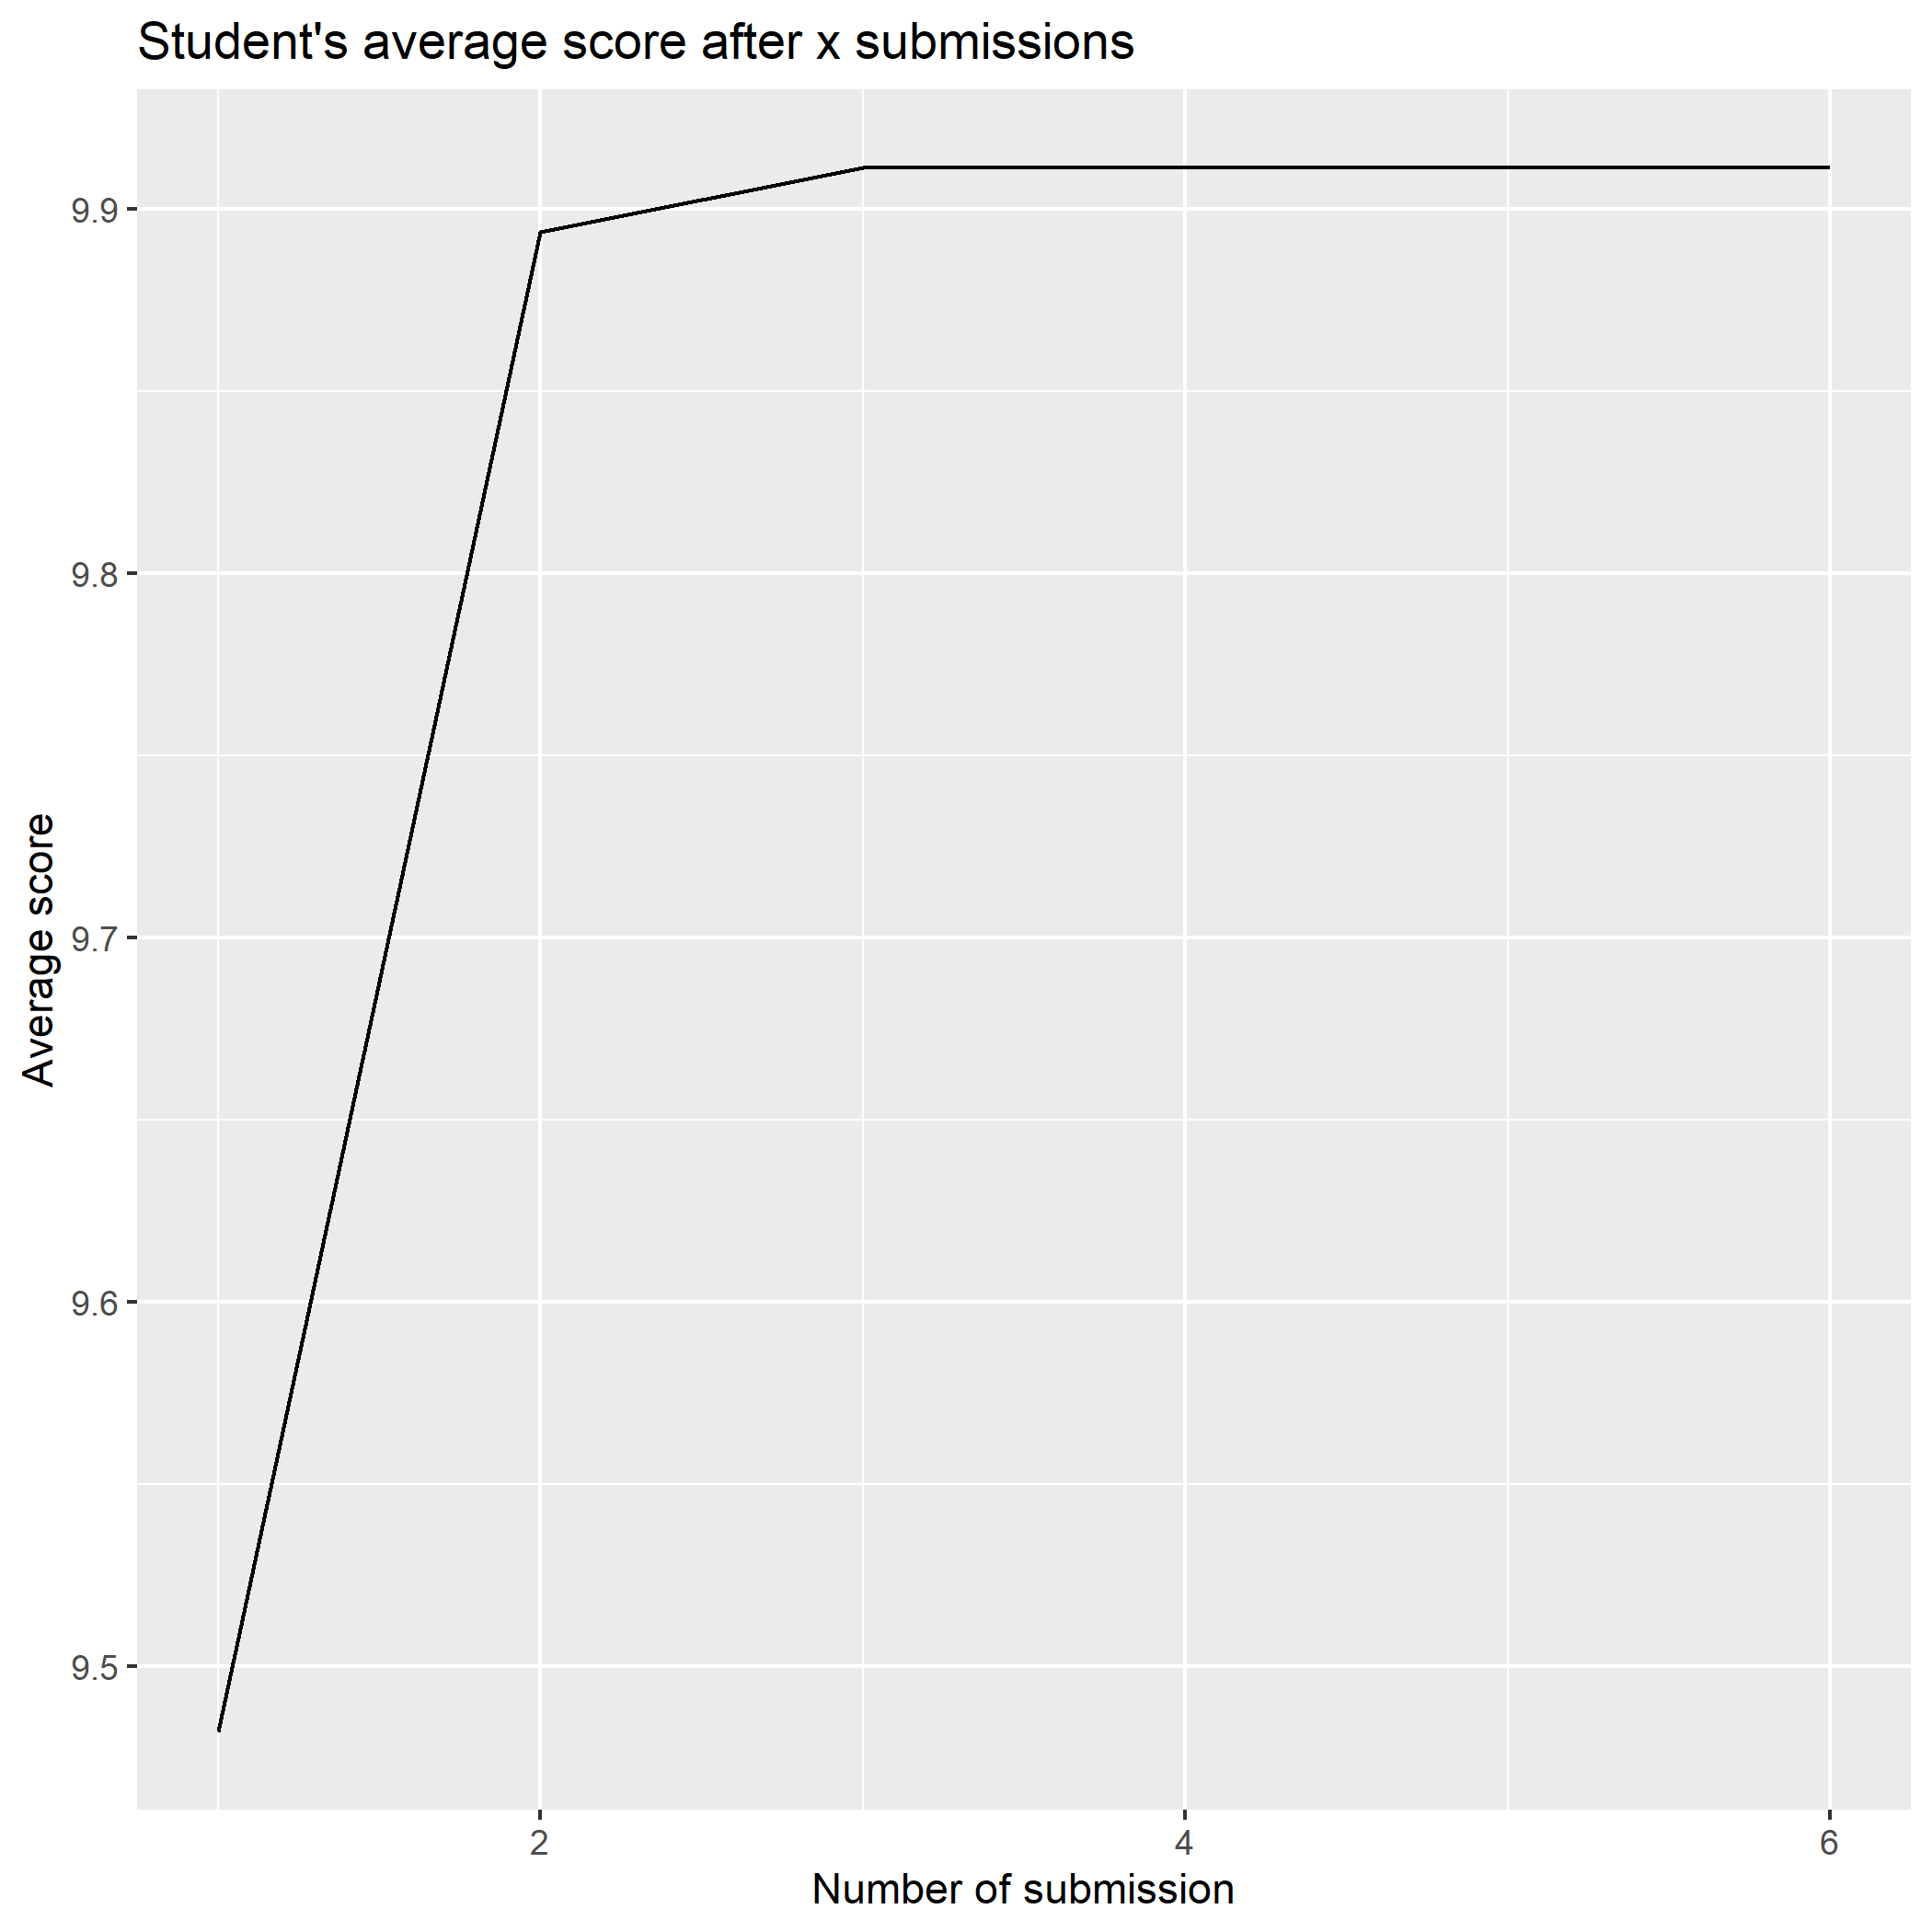
\includegraphics[scale=0.4]{Pics/q5c_file2.png}
    \caption{(5c) Điểm trung tất cả sinh viên tính theo sau k lần nộp}
    \label{fig:my_label}
\end{figure}

\newpage
\subsubsection{Câu 7}
\begin{figure}[!ht]
    \centering
    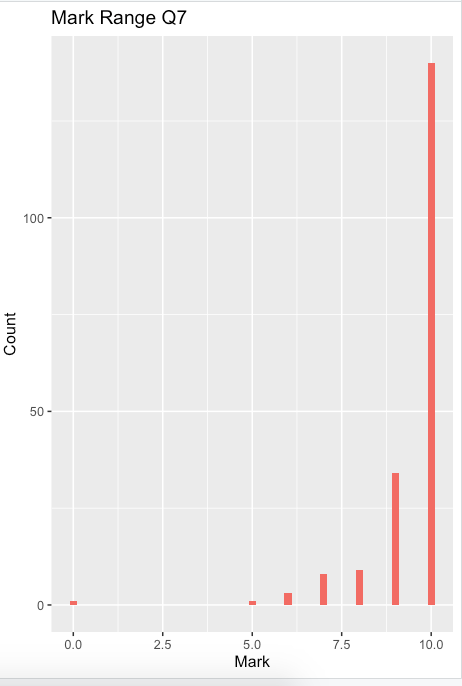
\includegraphics[scale=0.4]{Pics/q7-plot2.png}
    \caption{(7) Điểm trung tất cả sinh viên tính theo sau k lần nộp}
    \label{fig:my_label}
\end{figure}
\newpage
\subsubsection{Câu 9}
\begin{figure}[!ht]
    \centering
    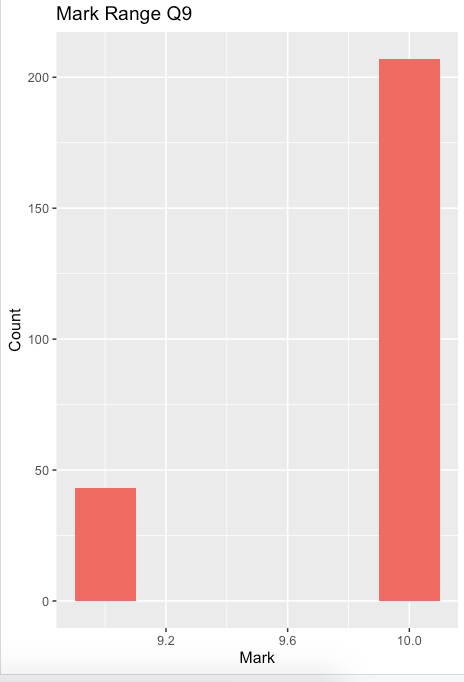
\includegraphics[scale=0.4]{Pics/q9-plot2.png}
    \caption{(9) Điểm trung tất cả sinh viên tính theo sau k lần nộp}
    \label{fig:my_label}
\end{figure}
\subsubsection{Câu 10}
\newpage
\subsubsection{Câu 10}
\newpage
\begin{figure}[!ht]
    \centering
    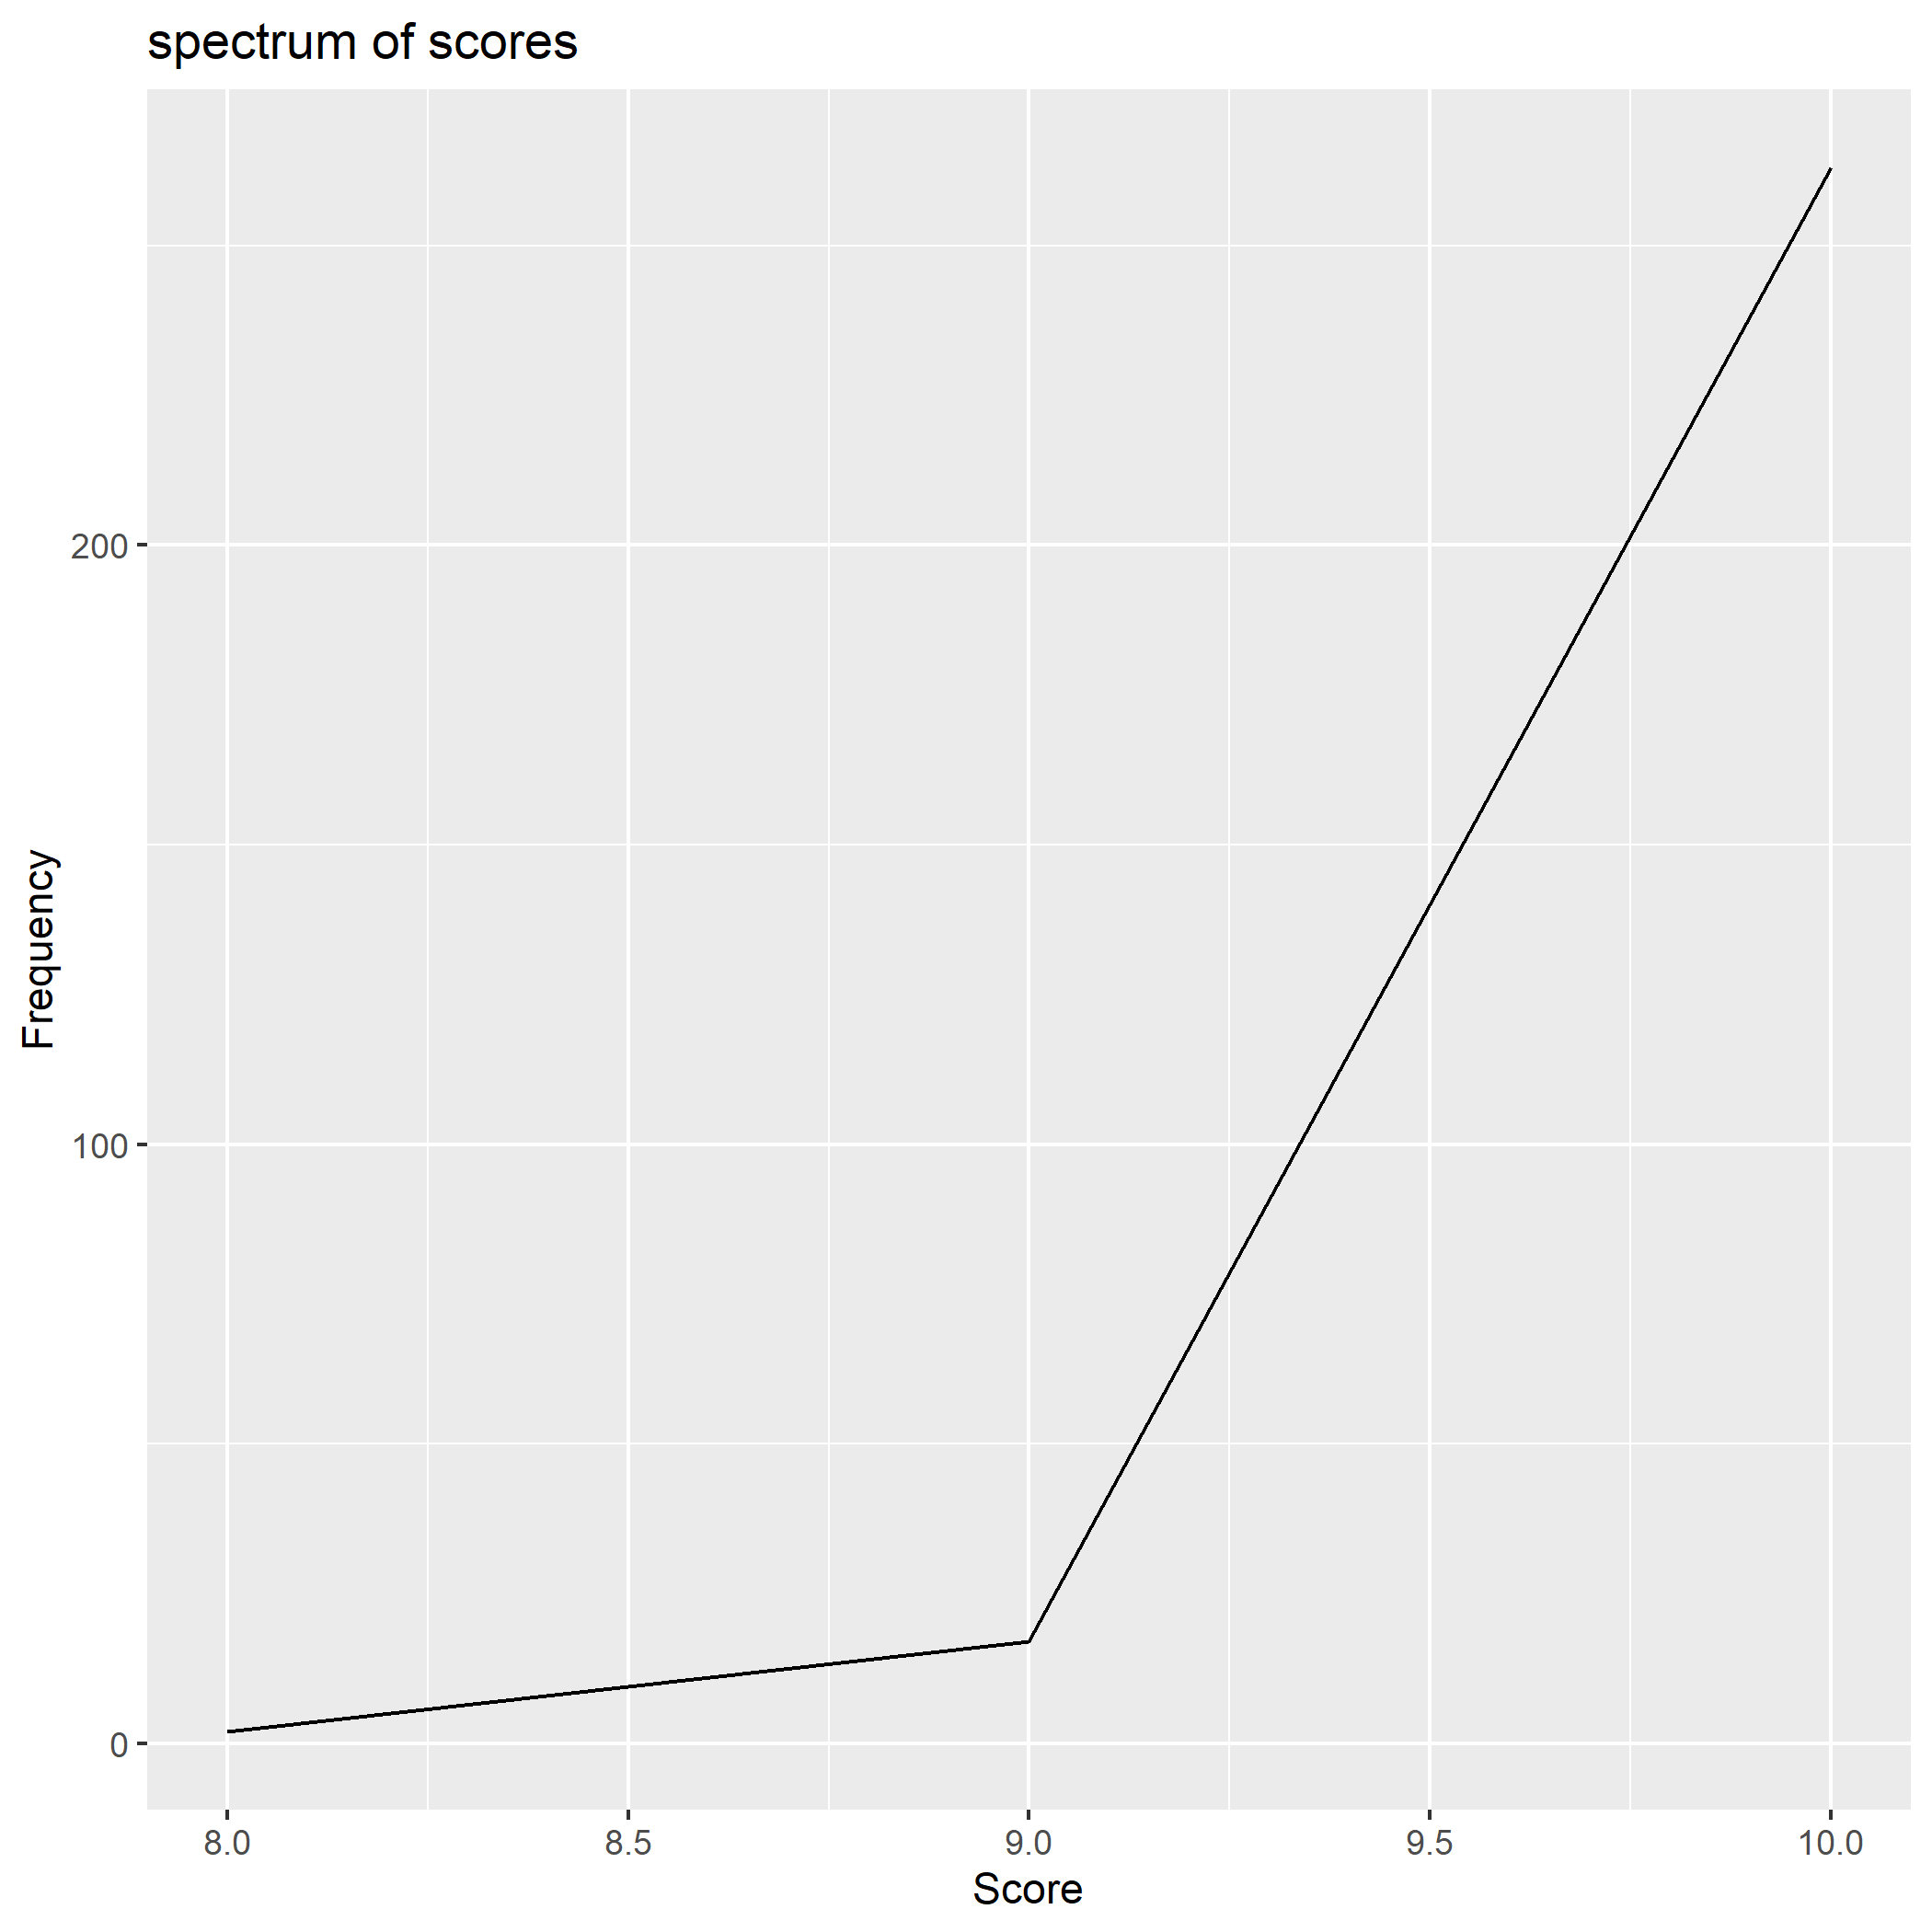
\includegraphics[scale=0.4]{Pics/q10c_file2.png}
    \caption{(10c) Phổ điểm sinh viên chủ động}
    \label{fig:my_label}
\end{figure}
\newpage
\subsubsection{Câu 11}

%%%%%%%%%%%%%%%%%%%%%%%%%%%%%%%%%%%%%%%%%%%%%%%%%%%
\newpage 
\subsection{File 3}
\textbf{$tid = 10$}\\
Các kết quả không phải đồ thị được lưu vào file $3.tsv$. Các kết quả đồ thị được biểu diễn tại đây
\subsubsection{Câu 1}
\subsubsection{Câu 2}
\begin{figure}[!ht]
    \centering
    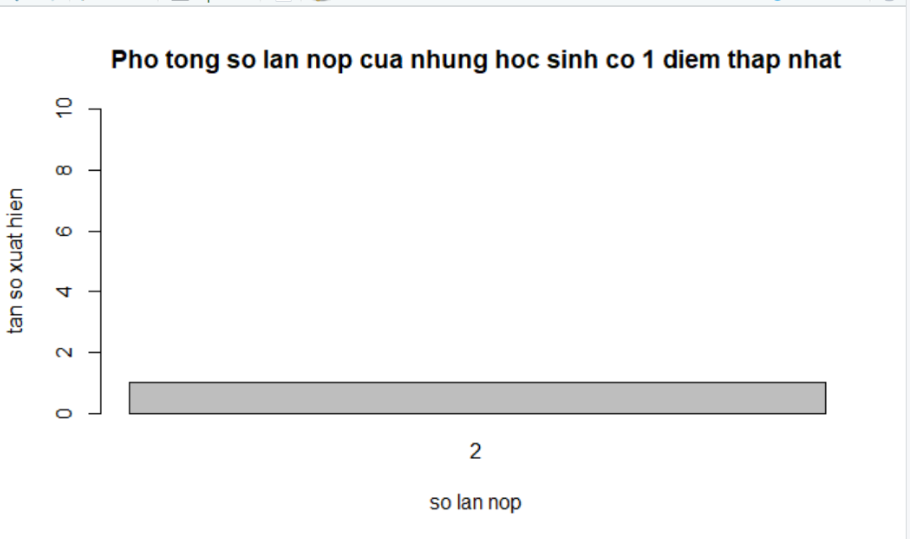
\includegraphics[scale=0.4]{Pics/q2d-file3.PNG}
    \caption{(2d) Phổ theo số lần nộp bài của sinh viên có ít nhất 1 bài nộp có điểm thấp nhất}
    \label{fig:my_label}
\end{figure}
\begin{figure}[!ht]
    \centering
    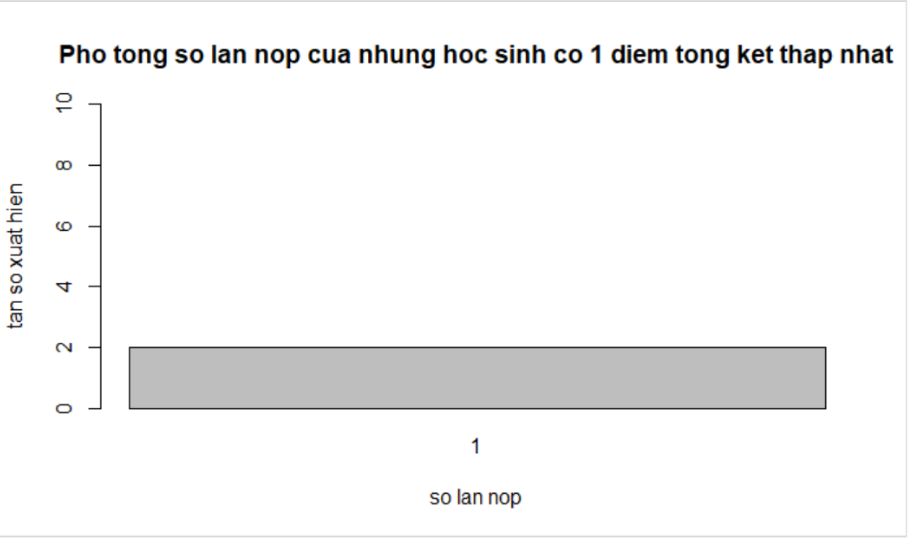
\includegraphics[scale=0.4]{Pics/q2g-file3.PNG}
    \caption{(2g) Phổ theo số lần nộp bài của các sinh viên có điểm số tổng kết thấp nhất }
    \label{fig:my_label}
\end{figure}
\newpage
\begin{figure}[!ht]
    \centering
    \includegraphics[scale=0.4]{Pics/q2j-file3.PNG}
    \caption{(2j)  Phổ theo số lần nộp bài của các sinh viên có tối thiểu một bài nộp có điểm số cao nhất}
    \label{fig:my_label}
\end{figure}
\begin{figure}[!ht]
    \centering
    \includegraphics[scale=0.4]{Pics/q2m-file3.PNG}
    \caption{(2m) Phổ theo số lần nộp bài của các sinh viên có điểm số tổng kết cao nhấtn}
    \label{fig:my_label}
\end{figure}
\begin{figure}[!ht]
    \centering
    \includegraphics[scale=0.4]{Pics/q2u-file3.PNG}
    \caption{(2u) Phổ theo số lần nộp bài của các sinh viên có điểm số tổng kết ở 2 mức điểm cao nhất}
    \label{fig:my_label}
\end{figure}
\newpage 
\begin{figure}[!ht]
    \centering
    \includegraphics[scale=0.4]{Pics/q2v-file3.PNG}
    \caption{(2v) Số lượng sinh viên có điểm số tổng kết ở mức điểm cao thứ $k$ với $k$ cho trước}
    \label{fig:my_label}
\end{figure}
\newpage
\begin{figure}[!ht]
    \centering
    \includegraphics[scale=0.4]{Pics/q2w-1-file3.png}
    \caption{(2w) Phổ theo số lần nộp bài của các sinh viên có điểm số tổng kết ở mức điểm cao thứ $1$}
    \label{fig:my_label}
\end{figure}
\begin{figure}[!ht]
    \centering
    \includegraphics[scale=0.4]{Pics/q2w-2-file3.png}
    \caption{(2w) Phổ theo số lần nộp bài của các sinh viên có điểm số tổng kết ở mức điểm cao thứ $2$}
    \label{fig:my_label}
\end{figure}
\begin{figure}[!ht]
    \centering
    \includegraphics[scale=0.4]{Pics/q2w-3-file3.png}
    \caption{(2w) Phổ theo số lần nộp bài của các sinh viên có điểm số tổng kết ở mức điểm cao thứ $3$}
    \label{fig:my_label}
\end{figure}
\begin{figure}[!ht]
    \centering
    \includegraphics[scale=0.4]{Pics/q2w-4-file3.png}
    \caption{(2w) Phổ theo số lần nộp bài của các sinh viên có điểm số tổng kết ở mức điểm cao thứ $4$}
    \label{fig:my_label}
\end{figure}
\begin{figure}[!ht]
    \centering
    \includegraphics[scale=0.4]{Pics/q2w-5-file3.png}
    \caption{(2w)Phổ theo số lần nộp bài của các sinh viên có điểm số tổng kết ở mức điểm cao thứ $5$}
    \label{fig:my_label}
\end{figure}
\newpage
\subsubsection{Câu 3}
\subsubsection{Câu 4}
\begin{figure}[!ht]
    \centering
    \includegraphics[scale=0.4]{Pics/q4b-file3.jpeg}
    \caption{(4b) Phổ thời gian làm việc (được tính từ lần nộp bài đầu tiên đến lần nộp cuối) của các
sinh viên.}
    \label{fig:my_label}
\end{figure}
\newpage
\begin{figure}[!ht]
    \centering
    \includegraphics[scale=0.4]{Pics/q4e-file3.jpeg}
    \caption{(4e) Phổ điểm của các sinh viên có tần suất nộp bài ít nhất}
    \label{fig:my_label}
\end{figure}
\begin{figure}[!ht]
    \centering
    \includegraphics[scale=0.4]{Pics/q4h-file3.jpeg}
    \caption{(4h) Phổ điểm của các sinh viên có tần suất nộp bài nhiều nhất}
    \label{fig:my_label}
\end{figure}
\begin{figure}[!ht]
    \centering
    \includegraphics[scale=0.4]{Pics/q4m-file3.jpeg}
    \caption{(4m) Biểu đồ tần số của mẫu}
    \label{fig:my_label}
\end{figure}
\begin{figure}[!ht]
    \centering
    \includegraphics[scale=0.4]{Pics/q4n-file3.jpeg}
    \caption{(4n) Biểu đồ tần suất của mẫu}
    \label{fig:my_label}
\end{figure}
\newpage
\begin{figure}[!ht]
    \centering
    \includegraphics[scale=0.4]{Pics/q4o-file3.jpeg}
    \caption{(4o) Biểu đồ tần suất tích lũy của mẫu }
    \label{fig:my_label}
\end{figure}
\subsubsection{Câu 5}
\begin{figure}[!ht]
    \centering
    \includegraphics[scale=0.4]{Pics/q5a_file3.png}
    \caption{(5a) Điểm sinh viên sau 6 lần nộp}
    \label{fig:my_label}
\end{figure}
\begin{figure}[!ht]
    \centering
    \includegraphics[scale=0.4]{Pics/q5b_file3.png}
    \caption{(5b) Điểm sinh viên sau 3 lần nộp}
    \label{fig:my_label}
\end{figure}
\begin{figure}[!ht]
    \centering
    \includegraphics[scale=0.4]{Pics/q5c_file3.png}
    \caption{(5c) Điểm trung tất cả sinh viên tính theo sau k lần nộp}
    \label{fig:my_label}
\end{figure}

\newpage
\subsubsection{Câu 7}
\begin{figure}[!ht]
    \centering
    \includegraphics[scale=0.4]{Pics/q7-plot3.png}
    \caption{(7) Điểm trung tất cả sinh viên tính theo sau k lần nộp}
    \label{fig:my_label}
\end{figure}
\newpage
\subsubsection{Câu 9}
\begin{figure}[!ht]
    \centering
    \includegraphics[scale=0.4]{Pics/q9-plot3.png}
    \caption{(9) Điểm trung tất cả sinh viên tính theo sau k lần nộp}
    \label{fig:my_label}
\end{figure}
\subsubsection{Câu 10}
\newpage
\subsubsection{Câu 10}
\newpage
\begin{figure}[!ht]
    \centering
    \includegraphics[scale=0.4]{Pics/q10c_file3.png}
    \caption{(10c) Phổ điểm sinh viên chủ động}
    \label{fig:my_label}
\end{figure}
\newpage
\subsubsection{Câu 11}

%%%%%%%%%%%%%%%%%%%%%%%%%%%%%%%%%%%%%%%%%%%%%%%%%%%
\newpage 
\subsection{File 4}\textbf{$tid = 8$}\\
Các kết quả không phải đồ thị được lưu vào file $4.tsv$. Các kết quả đồ thị được biểu diễn tại đây
\subsubsection{Câu 1}
\subsubsection{Câu 2}
\begin{figure}[!ht]
    \centering
    \includegraphics[scale=0.4]{Pics/q2d-file4.PNG}
    \caption{(2d) Phổ theo số lần nộp bài của sinh viên có ít nhất 1 bài nộp có điểm thấp nhất}
    \label{fig:my_label}
\end{figure}
\begin{figure}[!ht]
    \centering
    \includegraphics[scale=0.4]{Pics/q2g-file4.PNG}
    \caption{(2g) Phổ theo số lần nộp bài của các sinh viên có điểm số tổng kết thấp nhất }
    \label{fig:my_label}
\end{figure}
\newpage
\begin{figure}[!ht]
    \centering
    \includegraphics[scale=0.4]{Pics/q2j-file4.PNG}
    \caption{(2j)  Phổ theo số lần nộp bài của các sinh viên có tối thiểu một bài nộp có điểm số cao nhất}
    \label{fig:my_label}
\end{figure}
\begin{figure}[!ht]
    \centering
    \includegraphics[scale=0.4]{Pics/q2m-file4.PNG}
    \caption{(2m) Phổ theo số lần nộp bài của các sinh viên có điểm số tổng kết cao nhấtn}
    \label{fig:my_label}
\end{figure}
\begin{figure}[!ht]
    \centering
    \includegraphics[scale=0.4]{Pics/q2u-file4.PNG}
    \caption{(2u) Phổ theo số lần nộp bài của các sinh viên có điểm số tổng kết ở 2 mức điểm cao nhất}
    \label{fig:my_label}
\end{figure}
\newpage 
\begin{figure}[!ht]
    \centering
    \includegraphics[scale=0.4]{Pics/q2v-file4.PNG}
    \caption{(2v) Số lượng sinh viên có điểm số tổng kết ở mức điểm cao thứ $k$ với $k$ cho trước}
    \label{fig:my_label}
\end{figure}
\newpage
\begin{figure}[!ht]
    \centering
    \includegraphics[scale=0.4]{Pics/q2w-1-file4.png}
    \caption{(2w) Phổ theo số lần nộp bài của các sinh viên có điểm số tổng kết ở mức điểm cao thứ $1$}
    \label{fig:my_label}
\end{figure}
\begin{figure}[!ht]
    \centering
    \includegraphics[scale=0.4]{Pics/q2w-2-file4.png}
    \caption{(2w) Phổ theo số lần nộp bài của các sinh viên có điểm số tổng kết ở mức điểm cao thứ $2$}
    \label{fig:my_label}
\end{figure}
\begin{figure}[!ht]
    \centering
    \includegraphics[scale=0.4]{Pics/q2w-3-file4.png}
    \caption{(2w) Phổ theo số lần nộp bài của các sinh viên có điểm số tổng kết ở mức điểm cao thứ $3$}
    \label{fig:my_label}
\end{figure}
\begin{figure}[!ht]
    \centering
    \includegraphics[scale=0.4]{Pics/q2w-4-file4.png}
    \caption{(2w) Phổ theo số lần nộp bài của các sinh viên có điểm số tổng kết ở mức điểm cao thứ $4$}
    \label{fig:my_label}
\end{figure}
\begin{figure}[!ht]
    \centering
    \includegraphics[scale=0.4]{Pics/q2w-5-file4.png}
    \caption{(2w)Phổ theo số lần nộp bài của các sinh viên có điểm số tổng kết ở mức điểm cao thứ $5$}
    \label{fig:my_label}
\end{figure}
\newpage
\subsubsection{Câu 3}
\subsubsection{Câu 4}
\begin{figure}[!ht]
    \centering
    \includegraphics[scale=0.4]{Pics/q4b-file1.jpeg}
    \caption{(4b) Phổ thời gian làm việc (được tính từ lần nộp bài đầu tiên đến lần nộp cuối) của các
sinh viên.}
    \label{fig:my_label}
\end{figure}
\newpage
\begin{figure}[!ht]
    \centering
    \includegraphics[scale=0.4]{Pics/q4e-file4.jpeg}
    \caption{(4e) Phổ điểm của các sinh viên có tần suất nộp bài ít nhất}
    \label{fig:my_label}
\end{figure}
\begin{figure}[!ht]
    \centering
    \includegraphics[scale=0.4]{Pics/q4h-file4.jpeg}
    \caption{(4h) Phổ điểm của các sinh viên có tần suất nộp bài nhiều nhất}
    \label{fig:my_label}
\end{figure}
\begin{figure}[!ht]
    \centering
    \includegraphics[scale=0.4]{Pics/q4m-file4.jpeg}
    \caption{(4m) Biểu đồ tần số của mẫu}
    \label{fig:my_label}
\end{figure}
\begin{figure}[!ht]
    \centering
    \includegraphics[scale=0.4]{Pics/q4n-file4.jpeg}
    \caption{(4n) Biểu đồ tần suất của mẫu}
    \label{fig:my_label}
\end{figure}
\newpage
\begin{figure}[!ht]
    \centering
    \includegraphics[scale=0.4]{Pics/q4o-file4.jpeg}
    \caption{(4o) Biểu đồ tần suất tích lũy của mẫu }
    \label{fig:my_label}
\end{figure}
\subsubsection{Câu 5}
\begin{figure}[!ht]
    \centering
    \includegraphics[scale=0.4]{Pics/q5a_file1.png}
    \caption{(5a) Điểm sinh viên sau 6 lần nộp}
    \label{fig:my_label}
\end{figure}
\begin{figure}[!ht]
    \centering
    \includegraphics[scale=0.4]{Pics/q5b_file1.png}
    \caption{(5b) Điểm sinh viên sau 3 lần nộp}
    \label{fig:my_label}
\end{figure}
\begin{figure}[!ht]
    \centering
    \includegraphics[scale=0.4]{Pics/q5c_file1.png}
    \caption{(5c) Điểm trung tất cả sinh viên tính theo sau k lần nộp}
    \label{fig:my_label}
\end{figure}

\newpage
\subsubsection{Câu 7}
\begin{figure}[!ht]
    \centering
    \includegraphics[scale=0.4]{Pics/q7-plot1.png}
    \caption{(7) Điểm trung tất cả sinh viên tính theo sau k lần nộp}
    \label{fig:my_label}
\end{figure}
\newpage
\subsubsection{Câu 9}
\begin{figure}[!ht]
    \centering
    \includegraphics[scale=0.4]{Pics/q9-plot1.png}
    \caption{(9) Điểm trung tất cả sinh viên tính theo sau k lần nộp}
    \label{fig:my_label}
\end{figure}
\subsubsection{Câu 10}
\newpage
\subsubsection{Câu 10}
\newpage
\begin{figure}[!ht]
    \centering
    \includegraphics[scale=0.4]{Pics/q10c_file4.png}
    \caption{(10c) Phổ điểm sinh viên chủ động}
    \label{fig:my_label}
\end{figure}
\newpage
\subsubsection{Câu 11}

%%%%%%%%%%%%%%%%%%%%%%%%%%%%%%%%%%%%%%%%%%%%%%%%%%%%%%%%%%%%%%%%%%%%%%%%%%%%%%%%%%%%%%%%%%%%%%%%%%%
\end{document}